%%%%%%%%%%%%%%%%%%%%%%%%%%%%%%%%%%%%%%%%%
% Masters/Doctoral Thesis 
% LaTeX Template
% Version 2.5 (27/8/17)
%
% This template was downloaded from:
% http://www.LaTeXTemplates.com
%
% Version 2.x major modifications by:
% Vel (vel@latextemplates.com)
%
% This template is based on a template by:
% Steve Gunn (http://users.ecs.soton.ac.uk/srg/softwaretools/document/templates/)
% Sunil Patel (http://www.sunilpatel.co.uk/thesis-template/)
%
% Template license:
% CC BY-NC-SA 3.0 (http://creativecommons.org/licenses/by-nc-sa/3.0/)
%
%%%%%%%%%%%%%%%%%%%%%%%%%%%%%%%%%%%%%%%%%

%----------------------------------------------------------------------------------------
%	PACKAGES AND OTHER DOCUMENT CONFIGURATIONS
%----------------------------------------------------------------------------------------

\documentclass[uplatex,
12pt, % The default document font size, options: 10pt, 11pt, 12pt
%oneside, % Two side (alternating margins) for binding by default, uncomment to switch to one side
a4paper,
english, % ngerman for German
oneside,
titlepage,
%onehalfspacing,
singlespacing, % Single line spacing, alternatives: onehalfspacing or doublespacing
%draft, % Uncomment to enable draft mode (no pictures, no links, overfull hboxes indicated)
%nolistspacing, % If the document is onehalfspacing or doublespacing, uncomment this to set spacing in lists to single
liststotoc, % Uncomment to add the list of figures/tables/etc to the table of contents
%toctotoc, % Uncomment to add the main table of contents to the table of contents
%parskip, % Uncomment to add space between paragraphs
%nohyperref, % Uncomment to not load the hyperref package
headsepline,
% Uncomment to get a line under the header
%chapterinoneline, % Uncomment to place the chapter title next to the number on one line
%consistentlayout, % Uncomment to change the layout of the declaration, abstract and acknowledgements pages to match the default layout
]{MastersDoctoralThesis} % The class file specifying the document structure
\usepackage{CJKutf8} % Japanese
%\usepackage{xeCJK}
\usepackage{pdfpages}
\usepackage{bibentry} 
\usepackage{titlesec}

%\usepackage[T1]{fontenc}
\usepackage[utf8]{inputenc} % Required for inputting international characters
%usepackage[T1]{fontenc} % Output font encoding for international characters
%usepackage{termes}

\usepackage{mathptmx} % Use the Times font by default

\usepackage[backend=bibtex,style=ieee,natbib=true, maxnames=10, sorting=none]{biblatex} % Use the bibtex backend with the authoryear citation style (which resembles APA)
\usepackage[autostyle=true]{csquotes}

\usepackage{pgfplotstable} %e \pgfplotstabletypeset[options]{file}.

%\usepackage{caption}
\usepackage{grffile}
\usepackage{float}
\usepackage{subfigure}
\usepackage{url}
\usepackage{textcomp}
\usepackage[strings]{underscore}
\usepackage{svg}
%\usepackage{subcaption}
\addbibresource{bibliography.bib} % The filename of the bibliography




\usepackage{graphicx}
\graphicspath{ {figures/} }
\usepackage{array}
\usepackage[autostyle=true]{csquotes} % Required to generate language-dependent quotes in the bibliography

%\usepackage{lineno,hyperref}
\usepackage[export]{adjustbox}
\usepackage{algorithmic}
\usepackage{algorithm}
\usepackage{amsmath}
\usepackage{diagbox}
\usepackage{multirow}
\usepackage[title]{appendix}
\setcounter{tocdepth}{1}
%\usepackage[dvipdfmx]{graphicx}

%\usepackage{fancyhdr}
%\pagestyle{fancy}
%----------------------------------------------------------------------------------------
%	MARGIN SETTINGS
%----------------------------------------------------------------------------------------
\pretolerance=3000
\tolerance=200
\emergencystretch=0pt
\righthyphenmin=4
\lefthyphenmin=4
%\usepackage{microtype}




\geometry{
	paper=a4paper, % Change to letterpaper for US letter
	inner=2.5cm, % Inner margin
	outer=3.8cm, % Outer margin
	bindingoffset=.5cm, % Binding offset
	top=1.5cm, % Top margin
	bottom=1.5cm, % Bottom margin
	%showframe, % Uncomment to show how the type block is set on the page
}

%----------------------------------------------------------------------------------------
%	THESIS INFORMATION
%----------------------------------------------------------------------------------------

\thesistitle{Development of a Wearable Haptic Feedback Device for Enhancing Immersion in Virtual Reality} % Your thesis title, this is used in the title and abstract, print it elsewhere with \ttitle
\supervisor{Makio Ishihara} % Your supervisor's name, this is used in the title page, print it elsewhere with \supname
\examiner{} % Your examiner's name, this is not currently used anywhere in the template, print it elsewhere with \examname
\degree{Master} % Your degree name, this is used in the title page and abstract, print it elsewhere with \degreename
\author{Korntawat Witchuvanit} % Your name, this is used in the title page and abstract, print it elsewhere with \authorname
\addresses{} % Your address, this is not currently used anywhere in the template, print it elsewhere with \addressname

\subject{Engineering} % Your subject area, this is not currently used anywhere in the template, print it elsewhere with \subjectname
\keywords{} % Keywords for your thesis, this is not currently used anywhere in the template, print it elsewhere with \keywordnames
\university{\href{https://www.fit.ac.jp}{
		Fukuoka Institute of Technology}} % Your university's name and URL, this is used in the title page and abstract, print it elsewhere with \univname
\department{Graduate School of Engineering} % Your department's name and URL, this is used in the title page and abstract, print it elsewhere with \deptname
\group{} % Your research group's name and URL, this is used in the title page, print it elsewhere with \groupname
\faculty{} % Your faculty's name and URL, this is used in the title page and abstract, print it elsewhere with \facname

\AtBeginDocument{
\hypersetup{pdftitle=\ttitle} % Set the PDF's title to your title
\hypersetup{pdfauthor=\authorname} % Set the PDF's author to your name
\hypersetup{pdfkeywords=\keywordnames} % Set the PDF's keywords to your keywords
}

\begin{document}

\frontmatter % Use roman page numbering style (i, ii, iii, iv...) for the pre-content pages

\pagestyle{plain} % Default to the plain heading style until the thesis style is called for the body content

%----------------------------------------------------------------------------------------
%	TITLE PAGE
%----------------------------------------------------------------------------------------
\begin{titlepage}
\begin{center}

\begin{figure}[!t]
	\centering
	
\includegraphics[width=0.45\textwidth]{Pictures/fit.eps}
	\label{fig:logo}
	\vspace{-0.8cm}
\end{figure}

% \LARGE SEIKEI UNIVERSITY
% \vspace{10cm}
\textsc{Graduate School of Engineering Fukuoka Institute of Technology} \\

%\HRule

\vspace{1.0cm}
\begin{LARGE}
	
	\textbf{Master~Thesis}
	
	\vspace{+2.cm}
	
	
	\hrule height 2pt
	
	\vspace{+0.5cm}
		\textbf{Development of a Wearable Haptic Feedback Device for Enhancing Immersion in Virtual Reality}

	
	\vspace{+0.5cm}
	
	\hrule height 2pt
	
	\vspace{+3.0cm}
	
	
	
	Korntawat Wtichuvanit\\
	FM23201\\
	\vspace{+3.0cm}
	{\Large{
			Supervisor\\
			Prof.~Makio Ishihara \\
		}
	}
	
	\vspace{+1.5cm}
	

	
	{\Large July 2025  \\\vspace{+1cm}\Large Graduate School of Engineering \\Fukuoka Institute of Technology\\ Japan}
	
\end{LARGE}
\end{center}
\end{titlepage}

%----------------------------------------------------------------------------------------
%	DECLARATION PAGE
%----------------------------------------------------------------------------------------

%\begin{declaration}
%\addchaptertocentry{\authorshipname} % Add the declaration to the table of contents
%\noindent I, \authorname, declare that this thesis titled, \enquote{\ttitle} and the work presented in it are my own. I confirm that:

%\begin{itemize} 
%\item This work was done wholly or mainly while in candidature for a research degree at this University.
%\item Where any part of this thesis has previously been submitted for a degree or any other qualification at this University or any other institution, this has been clearly stated.
%\item Where I have consulted the published work of others, this is always clearly attributed.
%\item Where I have quoted from the work of others, the source is always given. With the exception of such quotations, this thesis is entirely my own work.
%\item I have acknowledged all main sources of help.
%\item Where the thesis is based on work done by myself jointly with others, I have made clear exactly what was done by others and what I have contributed myself.\\
%\end{itemize}
 
%\noindent Signed:\\
%\rule[0.5em]{25em}{0.5pt} % This prints a line for the signature
 
%\noindent Date:\\
%\rule[0.5em]{25em}{0.5pt} % This prints a line to write the date
%\end{declaration}

\cleardoublepage

%----------------------------------------------------------------------------------------
%	QUOTATION PAGE
%----------------------------------------------------------------------------------------

%\vspace*{0.2\textheight}

%\noindent\enquote{\itshape Thanks to my solid academic training, today I can write hundreds of words on virtually any topic without possessing a shred of information, which is how I got a good job in journalism.}\bigbreak

%\hfill Dave Barry

%----------------------------------------------------------------------------------------
%	ABSTRACT PAGE
%----------------------------------------------------------------------------------------

\begin{abstract}
\addchaptertocentry{\abstractname} % Add the abstract to the table of contents
Virtual reality (VR) provides immersive experiences through multisensory feedback, enhancing user interaction with digital environments. One key immersion aspect is texture rendering, which is commonly achieved through visual and auditory cues. Incorporating haptic feedback for realistic texture perception is a mainstream of Human-Computer Interaction (HCI) research activities and it remains a challenge. Most existing methods rely on hand-held devices, often limiting natural hand movements. This research explores the development and performance of a wearable device equipped with flex sensors, a Motion Processing Unit (MPU), and a coin motor, enabling texture perception at three vibration granularities. The results show that participants can distinguish various textures based on their smoothness, particularly identifying differences between them.

\vspace{5mm}


keyword: Human computer interaction (HCI), Texture Perception, Haptic devices
\end{abstract}
\clearpage
%----------------------------------------------------------------------------------------
%	ABSTRACT PAGE JP
%--------------------------------------------------------------------------------

\begin{abstract}

	%\renewcommand\abstractname{?��T?��v}

	\addchaptertocentry{\abstractname}
		% Add the abstract to the table of contents
		\begin{CJK*}{UTF8}{min}
			バーチャルリアリティ(VR)は、多感覚フィードバックによって没入型体験を提供し、ユーザーとデジタル環境とのインタラクションを向上させる。没入感を形成する重要な要素の一つがテクスチャの再現であり、一般的に視覚や聴覚を通じて提示されるが、リアルな質感を伝えるための触覚力を取り入れることはヒューマンコンピュータインタラクション(HCI)研究の主流であり、いまだに課題も多い。既存の手法の多くは手持ち式デバイスに依存するため、自然な手の動きを妨げることが多い。本研究では、フレックスセンサー、モーション処理ユニット(MPU)、およびコイン型振動モーターを備えたウェアラブルデバイスを開発し、3段階の振動粒度によるテクスチャ知覚の性能評価を行った。その結果、参加者は提示されたテクスチャの滑らかさに基づいて異なる質感を区別できること、特に各テクスチャ間の差異を識別可能であることが示された。
		\vspace{5mm}
		
		
		キーワード: ヒューマンコンピュータインタラクション(HCI)、テクスチャ知覚、触覚デバイス
		
		{\CJKfamily{mincho}}
	%	
		\end{CJK*}
	\end{abstract}

%----------------------------------------------------------------------------------------
%	ABSTRACT PAGE JP
%--------------------------------------------------------------------------------
%----------------------------------------------------------------------------------------
%	ACKNOWLEDGEMENTS
%----------------------------------------------------------------------------------------


%----------------------------------------------------------------------------------------
%	LIST OF CONTENTS/FIGURES/TABLES PAGES
%----------------------------------------------------------------------------------------

	\thispagestyle{empty}
	
	%\tableofcontents  % Prints the main table of contents
	%\tableofcontents[hideallsubsections]
	
    	\tableofcontents
	
	%\listoffigures % Prints the list of figures
	
	%\listoftables % Prints the list of tables
	
	\newpage
	
	\pagenumbering{arabic}
	
%----------------------------------------------------------------------------------------
%	ABBREVIATIONS
%----------------------------------------------------------------------------------------
%\begin{abbreviations}{ll} % Include a list of abbreviations (a table of two columns)

%\textbf{MAFF} & \textbf{M}inistry of \textbf{A}griculture, \textbf{F}orestry, and %\textbf{F}isheries\\
%\textbf{AI} & \textbf{A}rtificial \textbf{I}ntelligence

%\end{abbreviations}

%----------------------------------------------------------------------------------------
%	PHYSICAL CONSTANTS/OTHER DEFINITIONS
%----------------------------------------------------------------------------------------

%\begin{constants}{lr@{${}={}$}l} % The list of physical constants is a three column table

% The \SI{}{} command is provided by the siunitx package, see its documentation for instructions on how to use it

%Speed of Light & $c_{0}$ & \SI{2.99792458e8}{\meter\per\second} (exact)\\
%Constant Name & $Symbol$ & $Constant Value$ with units\\

%\end{constants}

%----------------------------------------------------------------------------------------
%	SYMBOLS
%----------------------------------------------------------------------------------------

%\begin{symbols}{lll} % Include a list of Symbols (a three column table)

%$a$ & distance & \si{\meter} \\
%$P$ & power & \si{\watt} (\si{\joule\per\second}) \\
%Symbol & Name & Unit \\

%\addlinespace % Gap to separate the Roman symbols from the Greek

%$\omega$ & angular frequency & \si{\radian} \\

%\end{symbols}

%----------------------------------------------------------------------------------------
%	DEDICATION
%----------------------------------------------------------------------------------------

%\dedicatory{For/Dedicated to/To my\ldots} 

%----------------------------------------------------------------------------------------
%	THESIS CONTENT - CHAPTERS
%----------------------------------------------------------------------------------------

\mainmatter % Begin numeric (1,2,3...) page numbering

\pagestyle{thesis} % Return the page headers back to the "thesis" style

% Include the chapters of the thesis as separate files from the Chapters folder
% Uncomment the lines as you write the chapters

% Chapter 1

\chapter{Introduction} % Main chapter title

\label{Chapter1} % For referencing the chapter elsewhere, use \ref{Chapter1} 

%----------------------------------------------------------------------------------------

% Define some commands to keep the formatting separated from the content 
\newcommand{\keyword}[1]{\textbf{#1}}
\newcommand{\tabhead}[1]{\textbf{#1}}
\newcommand{\code}[1]{\texttt{#1}}
\newcommand{\file}[1]{\texttt{\bfseries#1}}
\newcommand{\option}[1]{\texttt{\itshape#1}}

%----------------------------------------------------------------------------------------
This chapter presents backgrounds, objective, and the structure of this thesis.

\section{Backgrounds}
Virtual reality (VR) has evolved into a powerful platform that provides immersive experiences across various applications, including gaming, training simulations, healthcare, education, and therapy\cite{10.3389/frobt.2016.00074}. By integrating visual, auditory, and interactive elements, VR environments create a strong sense of presence, which significantly enhances user engagement and the perception of realism\cite{10.5555/207922}. Considerable advancements in display technologies, accurate motion tracking systems, and spatial audio reproduction have greatly improved user immersion. However, despite these technological advancements, achieving realistic tactile feedback remains a significant challenge, limiting the overall sensory fidelity and immersion in VR applications\cite{10.1146/annurev-control-060117-105043}.

To reduce the sensory gap, haptic feedback plays a vital role by providing tactile stimuli that replicate real-world touch sensations\cite{10.1146/annurev-control-060117-105043}. Various haptic devices, ranging from basic vibrotactile actuators to advanced force-feedback systems and wearable gloves, have been thoroughly explored to enhance tactile realism. While handheld controllers are commonly used due to their simplicity and practicality, they often restrict natural hand movements and hinder intuitive interactions with virtual objects, which can lead to a diminished sense of immersion. In contrast, wearable haptic solutions that directly integrate with the user's body present promising alternatives, allowing for natural and intuitive hand gestures and interactions\cite{7922602}. However, creating wearable devices that balance lightweight design, responsiveness, ergonomic comfort, and adaptability continues to be a significant challenge within Human-Computer Interaction (HCI) research.

To address these limitations, I propose the design and implementation of a custom wearable glove embedded with flex sensors that capture precise hand gestures, a Motion Processing Unit (MPU) for accurate movement tracking, and a coin motor to provide detailed haptic feedback. This glove has been specifically engineered to enhance the perception of virtual textures by utilizing vibrational feedback across three distinct levels of granularity, carefully chosen for their effectiveness in conveying realistic texture sensations\cite{10.1145/3025453.3025812}. The main contributions of this research include the successful development of a responsive and lightweight wearable haptic device, as well as a comprehensive empirical evaluation of user tactile perception across different vibration granularities. This work significantly advances the realism and immersive quality of haptic feedback systems in virtual reality.

%----------------------------------------------------------------------------------------

\section{Objective}

The objective of this research is to design and evaluate a lightweight and responsive wearable haptic glove that incorporates flex sensors, a Motion Processing Unit (MPU), and a coin motor. This glove aims to enhance the perception of realistic textures in virtual environments. By providing vibration feedback at three different levels of granularity, this study empirically assesses users' ability to accurately distinguish virtual textures based on perceived smoothness. Ultimately, this research seeks to advance tactile realism and improve overall immersion in virtual reality applications.

\section{Thesis structure}

This thesis consists of six chapters. Chapter~\ref{Chapter1}  introduces the background, objectives, and structure of the thesis. Chapter~\ref{Chapter2} provides a comprehensive review of related work in the field. Chapter~\ref{Chapter3} describes the design and implementation of a wearable haptic device that incorporates flex sensors, a coin motor, and an MPU. Chapter~\ref{Chapter4} outlines the experimental methodology and assesses the ability of users to distinguish various texture granularities. Chapter~\ref{Chapter5} presents the results and discusses practical considerations and potential real-world applications of the proposed device. Finally, Chapter~\ref{Chapter6} concludes the thesis and suggests directions for future research.




\chapter{Related work} % Main chapter title

\label{Chapter2} % Change X to a consecutive number; for referencing this chapter elsewhere, use \ref{ChapterX}


%----------------------------------------------------------------------------------------
%	SECTION 1
%----------------------------------------------------------------------------------------
\section{Haptic Feedback in VR}
Haptic feedback is a technology that provides tactile sensations to users, enabling them to physically feel virtual objects and interactions. In virtual reality, the lack of touch feedback can limit realism and diminish the sense of presence. To address this limitation, haptic feedback systems are integrated alongside visual and auditory cues, resulting in a richer and more immersive user experience. Haptic feedback allows users to perceive various object properties, such as texture, shape, stiffness, and temperature, which would otherwise be absent in digital environments~\cite{doi:10.34133/research.0333}.

\subsection{Vibrotactile Feedback}
Vibrotactile feedback is one of the most commonly used haptic methods in virtual reality, especially in wearable applications. This technique employs small vibrating actuators to create tactile sensations on the skin, enabling users to experience interactions such as contact with virtual objects, collision effects, surface textures, and environmental cues. Its popularity is due to several advantages, including compact size, low cost, energy efficiency, fast response times, and ease of integration into various wearable devices, such as gloves, vests, thimbles, and headgear.

Research consistently demonstrates that vibrotactile feedback effectively enhances user immersion. For instance, a study by Barsen et al.~\cite{10.1007/978-3-030-06134-0_25} on commercial VR systems equipped with vibrotactile vests revealed that participants reported significantly higher levels of co-presence and realism when vibrotactile cues were present during avatar collisions. Additionally, a review by H. Shiying~\cite{10.54254/2753-8818/17/20240650} confirmed that vibrotactile stimulation effectively conveys fine textures and surface variations, making it particularly suitable for VR texture-rendering tasks.

\newpage
\subsection{Force Feedback}
Force feedback is a key haptic technology that creates mechanical resistance to mimic the physical characteristics of virtual objects, such as weight, stiffness, and collision forces. This technology typically uses motors, gears, or mechanical linkages to generate opposing forces in response to user movements, enhancing the realism of physical interactions within virtual environments. Force feedback is commonly found in haptic exoskeleton gloves, joystick-based systems, and haptic robotic arms. It is particularly valuable in training simulators, rehabilitation, and virtual manipulation tasks where a realistic sense of force is essential.~\cite{10.3389/fbioe.2020.541105}

Numerous studies have shown that force feedback significantly improves user interaction and realism in virtual environments. Zhang et al.~\cite{zhang2025doglovedexterousmanipulationlowcost} introduced the DOGlove, a low-cost, open-source glove that provides five degrees of freedom (5-DoF) force feedback at the fingertips. This is achieved through compact, cable-driven torque systems, which enable high precision in teleoperation and underscore the crucial role of force feedback in contact-intensive robotic manipulation.

\subsection{Thermal Feedback}
Thermal feedback conveys sensations of temperature—whether warmth or coolness—through haptic interfaces, which enhances the realism of materials in virtual reality environments. By simulating the thermal properties of objects, users can distinguish virtual materials not only by touch but also by temperature, leading to more immersive interactions. Thermal actuators typically utilize Peltier thermoelectric elements or resistive heating pads, enabling dynamic temperature modulation in response to various virtual scenarios~\cite{TANG2024100365}.

Kang et al.~\cite{10.48550/arXiv.2405.11807} developed a dual-sided rotating Peltier module system that facilitates quick transitions between warm and cool stimuli, which is perfect for real-time VR applications. This system also enhances user comfort through the use of layered insulation.

%----------------------------------------------------------------------------------------
%	SECTION 2
%----------------------------------------------------------------------------------------
\newpage
\section{Texture Rendering}
Texture rendering in virtual reality aims to replicate the tactile sensations of various materials to create a realistic perception of surface properties. This process involves multiple sensory channels, including visual, auditory, and haptic feedback. Research consistently demonstrates that haptic feedback is crucial for authentic texture perception, especially in interactive VR applications. The objective of texture rendering is to enable users to identify and differentiate between virtual surfaces as naturally as they would with physical surfaces. This capability significantly enhances the sense of presence, immersion, and realism in VR environments.
\begin{figure}[H]\centering
	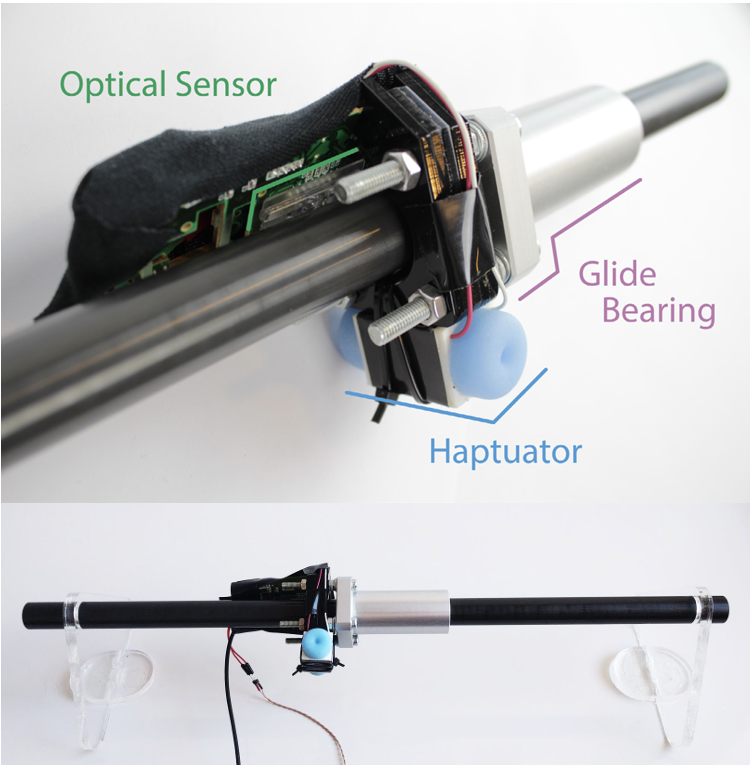
\includegraphics[width=0.6\textwidth]{Pictures/Texture_Rendering_1.png}%imagine location
	\caption{Slider used for experiment. Participants interact with slider by moving the silver glide bearing~\cite{10.1145/3025453.3025812}}\label{fig:Texture_Rendering_1}%use name for ref.
\end{figure}

P. Strohmeier et al. ~~\cite{10.1145/3025453.3025812} proposed a method for generating haptic textures by integrating vibrotactile feedback with user movement. Their approach is based on the idea that texture perception in real-world interactions arises from active exploration, with vibrations produced by the relative motion between the finger and the surface. To simulate this mechanism, they developed a custom haptic interface, as shown in Fig.~\ref{fig:Texture_Rendering_1}. This interface incorporates a linear slider, a BM3C Haptuator, an optical position sensor, and features minimal mechanical friction to avoid interference from passive forces.

The study explored four dimensions of perceptual texture: roughness, bumpiness, sharpness, and adhesiveness. These dimensions are consistent with established theories of tactile perception~~\cite{6216375}.The authors systematically varied three key vibrotactile parameters(Fig.~\ref{fig:Texture_Rendering_2}): granularity, amplitude, and timbre. Participants took part in a magnitude estimation task, where they rated the intensity of perceived textures based on different configurations of these parameters. The results revealed that granularity was the primary factor in distinguishing between textures in terms of roughness and bumpiness.

\begin{figure}[H]\centering
	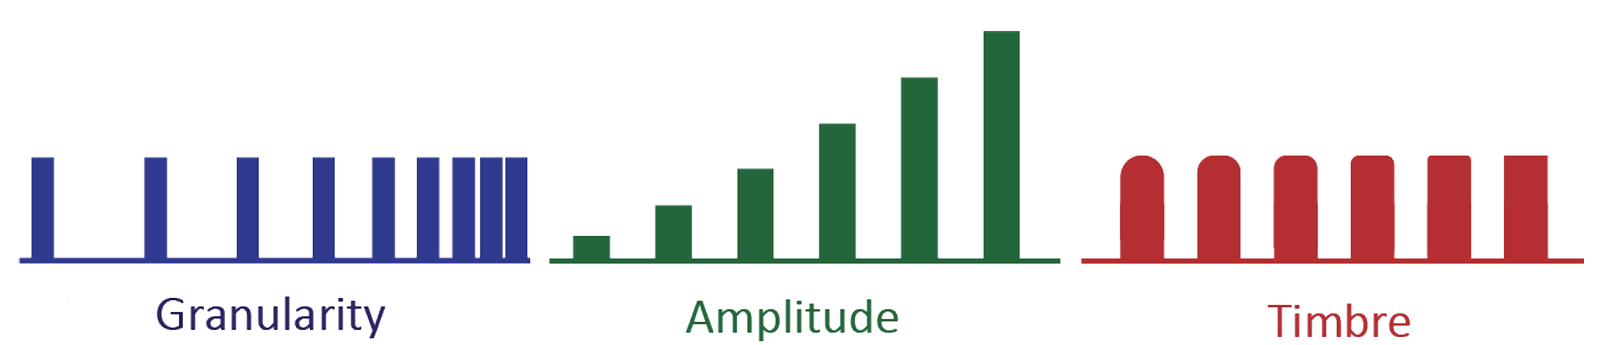
\includegraphics[width=1\textwidth]{Pictures/Texture_Rendering_2.png}%imagine location
	\caption{Naïve visualization of vibrotactile parameters~\cite{10.1145/3025453.3025812}}\label{fig:Texture_Rendering_2}%use name for ref.
\end{figure}

%----------------------------------------------------------------------------------------
%	SECTION 3
%----------------------------------------------------------------------------------------

\section{Research Gap and Positioning of This Work}
Previous studies in the field of haptic feedback for virtual reality have explored various methods to enhance tactile realism. Force-feedback systems provide mechanical resistance, allowing users to feel weight and stiffness. However, these systems are often bulky, complex, and can hinder mobility, making them unsuitable for lightweight wearable applications. Thermal feedback has also been used to simulate directionality and temperature cues, but it suffers from slow response times and limited surface coverage. In contrast, vibrotactile feedback has emerged as the most common approach due to its simplicity, low cost, and responsiveness. However, many studies still rely on amplitude or frequency modulation to represent contact events and basic textures.

This study, however, takes a different approach by focusing on cycle rate modulation using pulse-width modulation to convey the roughness and bumpiness of textures. Instead of modifying vibration amplitude or frequency, which often requires precise tuning of actuators, our method alters the rhythm (on-off timing) of vibration pulses to represent texture properties. This approach offers several practical advantages: it enables the use of a single actuator per finger, eliminates the need for complex multi-actuator arrays, and reduces hardware complexity while still producing clearly distinguishable tactile sensations associated with surface roughness and bumpiness. 

Furthermore, by relying solely on PWM cycle rate modulation, the system simplifies both hardware implementation and software control, making it particularly suitable for lightweight and real-time VR applications.

 
\chapter{Wearable Haptic Feedback Device} % Main chapter title

\label{Chapter3} % Change X to a consecutive number; for referencing this chapter elsewhere, use \ref{ChapterX}
\section{Proposed method}
This paper proposes a lightweight wearable haptic device designed to address the limitations of natural hand interactions and improve the perception of virtual textures. The primary objective is to create a cost-effective and responsive wearable system that enables users to manipulate virtual objects freely while receiving realistic vibrotactile feedback. The system's detailed architecture is illustrated in Fig.~\ref{fig:system_diagram}.

\begin{figure}[H]\centering
	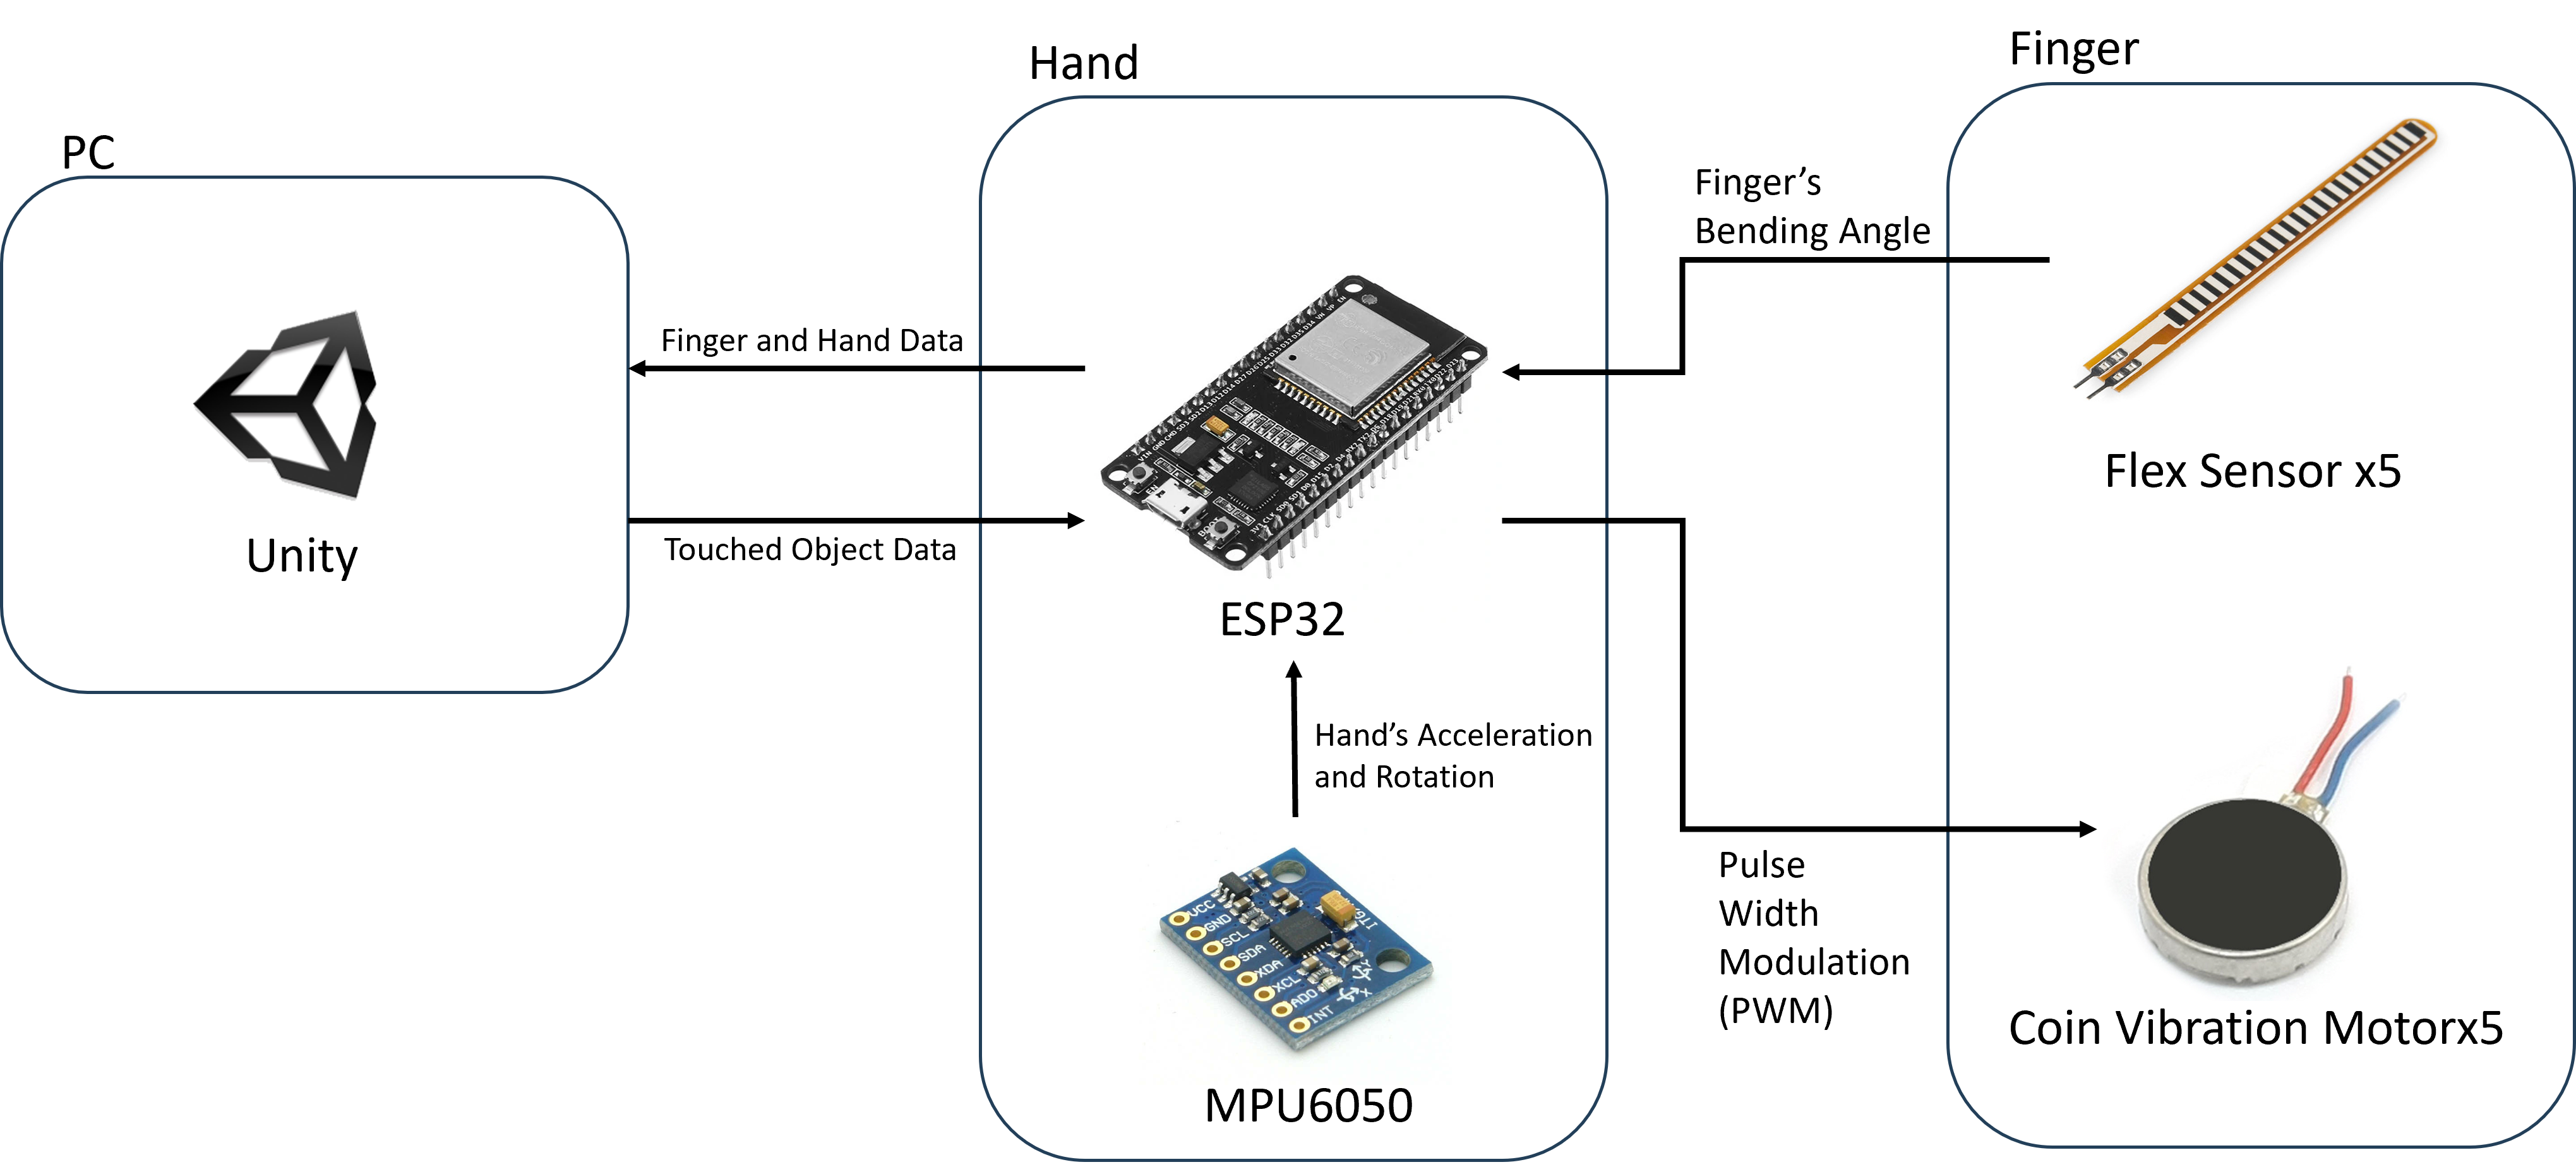
\includegraphics[width=1\textwidth]{Pictures/system_diagram.png}%imagine location
	\caption{System architecture of the wearable haptic glove, showing integration between Unity, ESP32, and hardware components.}\label{fig:system_diagram}%use name for ref.
\end{figure}
%%%%%%%%%%%%%%%%%%%%%%%%%%%%%%%%%%
\subsection{ESP32 Microcontroller}
The ESP32(Fig.~\ref{fig:esp32}) microcontroller serves as the central control unit for the proposed wearable haptic system. Developed by Espressif Systems, the ESP32 is a dual-core, low-power system-on-chip (SoC) designed for IoT and embedded applications. It offers a compact footprint, integrated Wi-Fi and Bluetooth connectivity, and extensive input/output (I/O) support~\cite{esp32docs}. With its small dimensions (approximately 25.5 mm × 18 mm for the ESP32-WROOM-32 variant), it is highly suitable for integration into wearable devices, where minimizing weight and bulk is essential.

\begin{figure}[H]\centering
	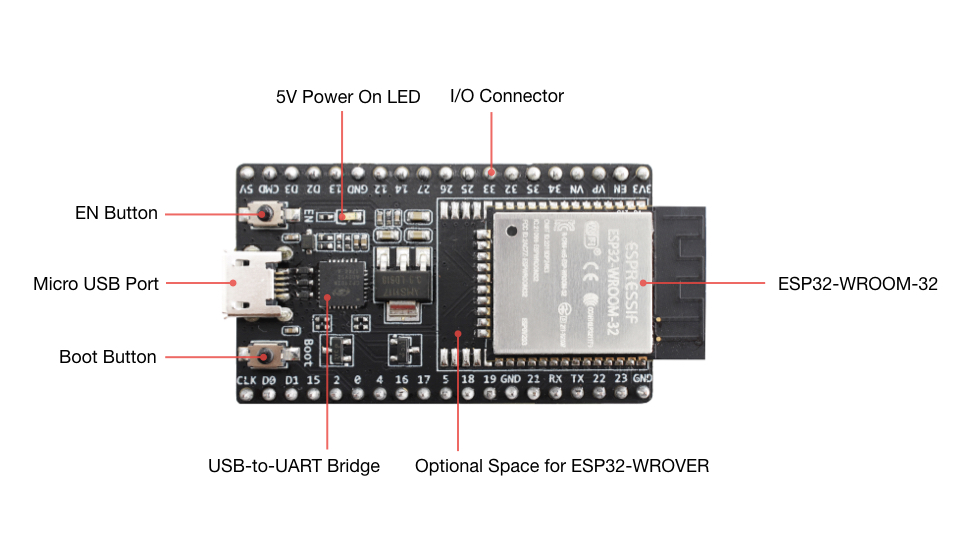
\includegraphics[width=1\textwidth]{Pictures/esp32.jpg}%imagine location
	\caption{ESP32-DevKitC V4 with ESP32-WROOM-32 module soldered~\cite{esp32docs}}\label{fig:esp32}%use name for ref.
\end{figure}

In the proposed system, the ESP32 is responsible for the real-time acquisition of hand motion and gesture data from the sensory module, which includes flex sensors and an Inertial Measurement Unit (IMU). It processes these signals and outputs Pulse Width Modulation (PWM) signals to control a vibrotactile actuator. Additionally, the ESP32 facilitates communication with the virtual reality environment, transmitting hand movement data and receiving feedback commands. This setup supports a low-latency and fully mobile VR haptic interaction system.
%%%%%%%%%%%%%%%%%

\newpage
\subsection{Flex Sensors}
Flex sensors(Fig.~\ref{fig:flex_sensor}) are the key components used to capture finger movements and hand gestures in the proposed wearable haptic device. These sensors are resistive, meaning their electrical resistance changes in proportion to how much they bend. When the sensor bends, the internal conductive particles inside it separate, leading to an increase in resistance. This property allows for direct and continuous analog measurements of finger flexion, facilitating the accurate real-time detection of hand postures.

\begin{figure}[H]\centering
	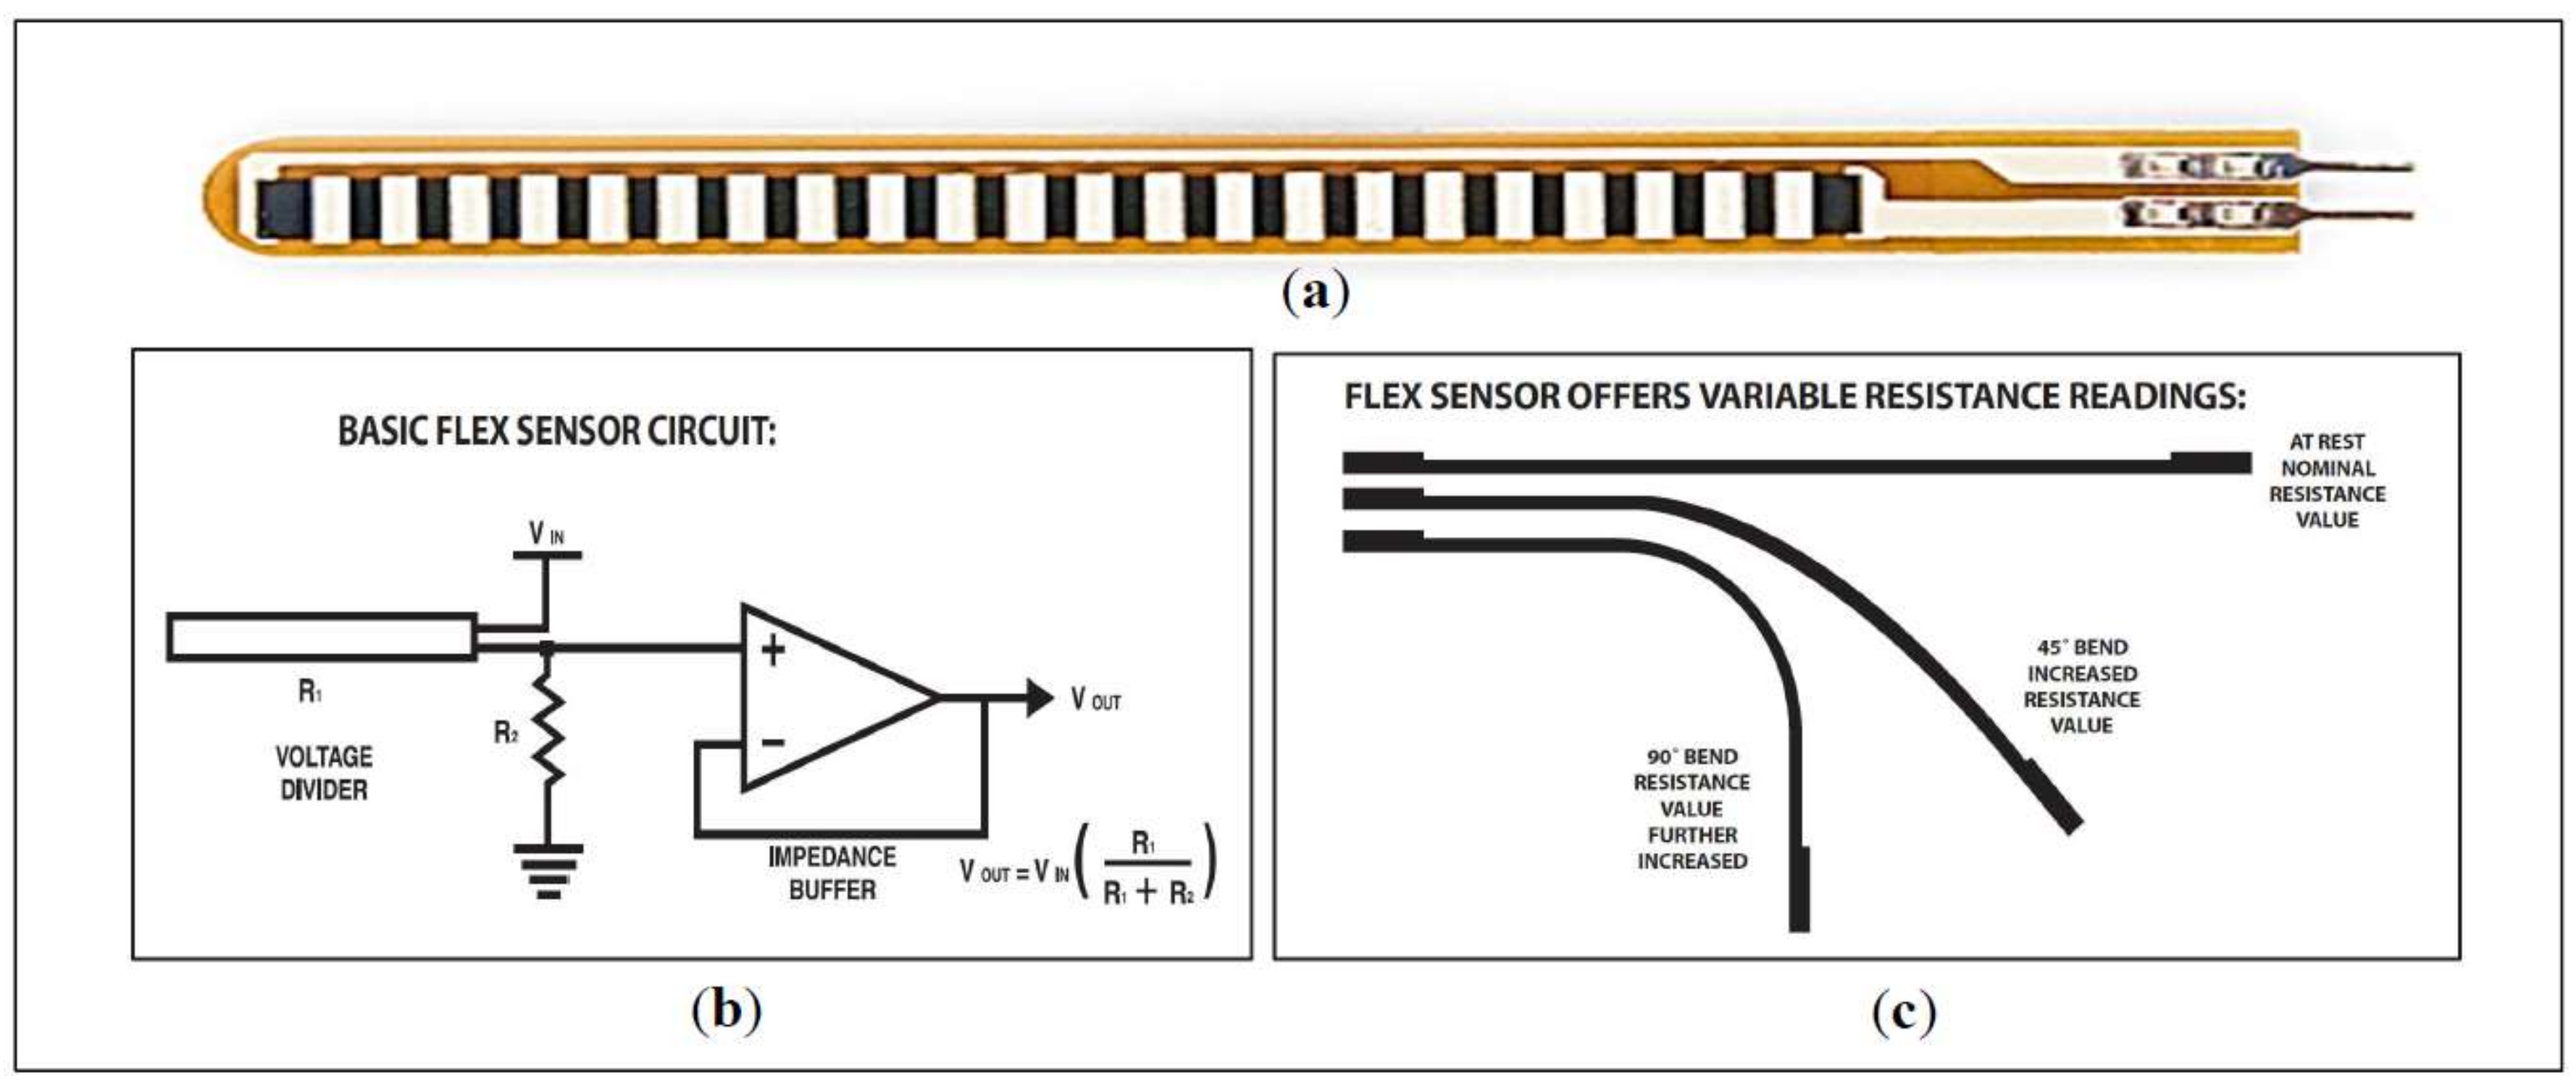
\includegraphics[width=1\textwidth]{Pictures/flex_sensor.png}%imagine location
	\caption{(a) Flex sensor, (b)voltage divider circuit, and (c) flex bend levels~\cite{10.3390/s18072208}}\label{fig:flex_sensor}%use name for ref.
\end{figure}

In this system,  flex sensors are attached along the dorsal side of each finger, from the base to the tip. Each flex sensor is incorporated into a voltage divider circuit, where it acts as the variable resistor. When a user flexes their finger, the corresponding change in resistance causes a drop in output voltage, which is sampled by the 12-bit ADC (Analog-to-Digital Converter) channels of the ESP32 microcontroller as shown in Fig.~\ref{fig:flex_sensor_bend}. This setup allows for precise real-time measurement of finger bending angles, translating physical finger positions into digital signals that can be used for gesture classification and interaction mapping within the VR environment.

\begin{figure}[H]\centering
	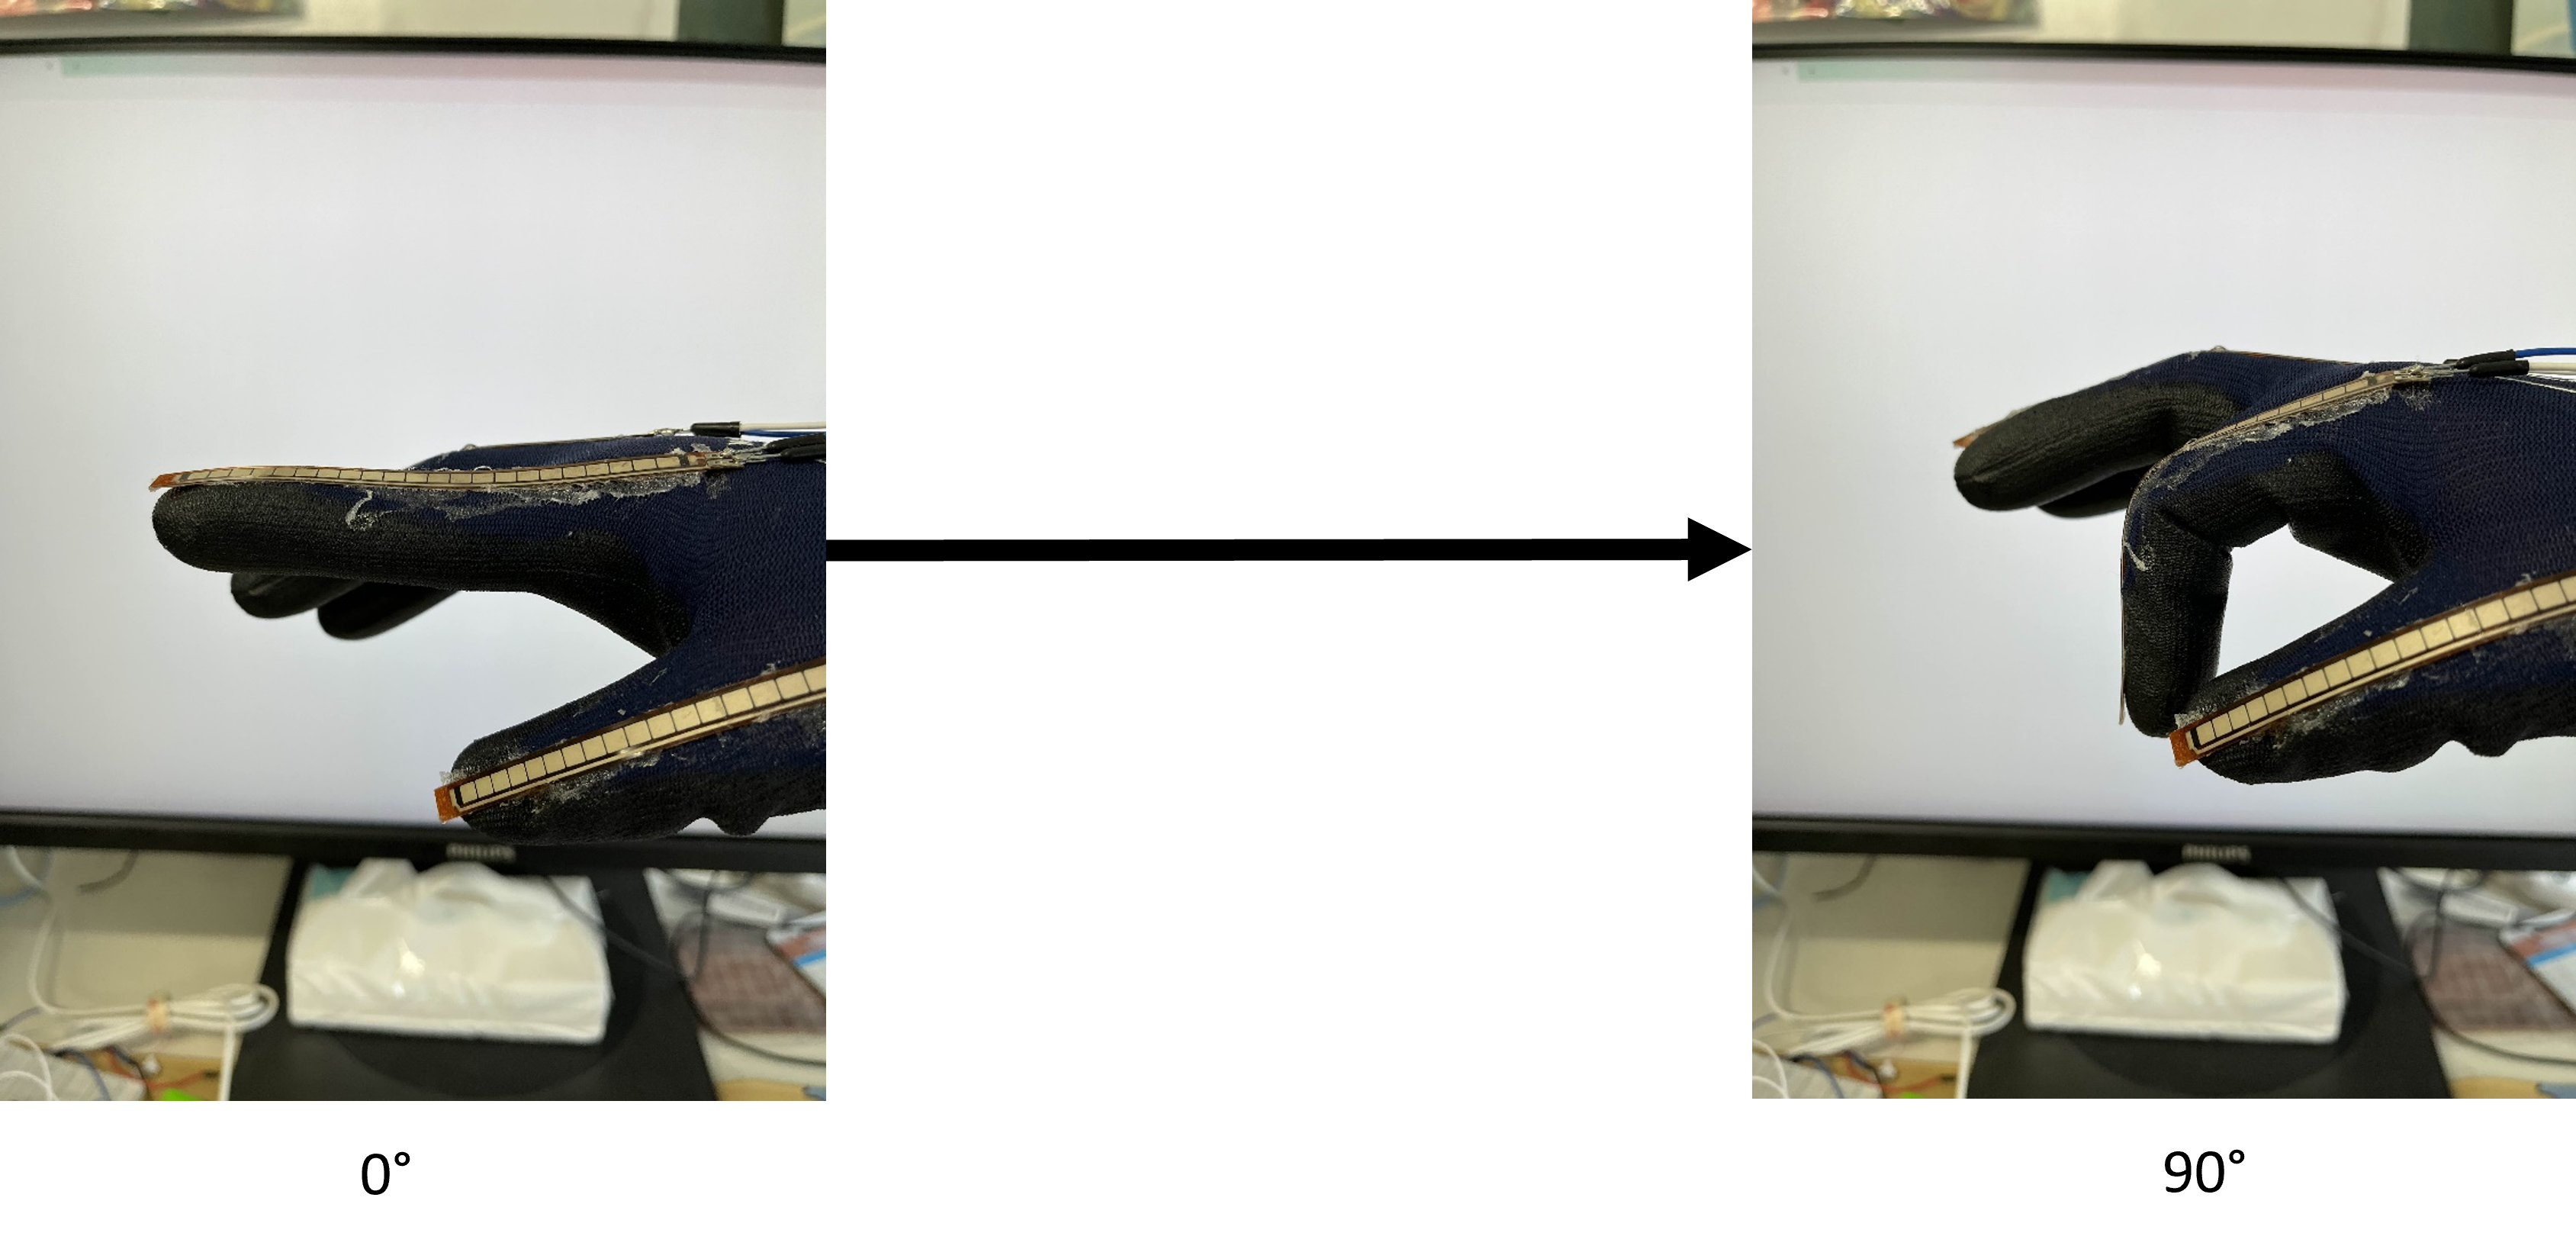
\includegraphics[width=1\textwidth]{Pictures/flex_sensor_bend.png}%imagine location
	\caption{Atteched flex sensor}\label{fig:flex_sensor_bend}%use name for ref.
\end{figure}

One of the main reasons for choosing flex sensors is their compact size, lightweight design, and mechanical flexibility. These features make them ideal for wearable applications as they do not hinder natural hand movements. Unlike vision-based tracking systems, flex sensors do not require external cameras or a direct line of sight, which ensures reliable tracking performance in various lighting conditions and during occluded hand interactions. Furthermore, flex sensors are energy-efficient and only draw a minimal amount of current, which contributes to a longer battery life for wearable devices.

By integrating flex sensors into the proposed device, the system accurately captures detailed finger movements, which are crucial for gesture recognition, interaction triggers, and texture manipulation tasks in virtual reality. The continuous, low-latency data obtained from the flex sensors complements the data from inertial measurement units, creating a multi-modal sensing system that enhances the realism of interactions with virtual objects.
%%%%%%%%%%%%%%%

\newpage
\subsection{Coin Vibration Motor}
The coin vibration motor(Fig.~\ref{fig:coin_motor}), known as the Eccentric Rotating Mass (ERM) type, is used as the main actuator to provide vibrotactile feedback in the proposed wearable haptic device. This type of motor works by rapidly rotating an off-center mass attached to its shaft, which creates oscillations that produce tactile sensations on the skin. Coin motors are favored in wearable devices due to their compact circular shape, lightweight (typically weighing under 3 grams per motor), and straightforward driving circuitry. These features make them ideal for applications where form factor and mobility are crucial design considerations.

\begin{figure}[H]\centering
	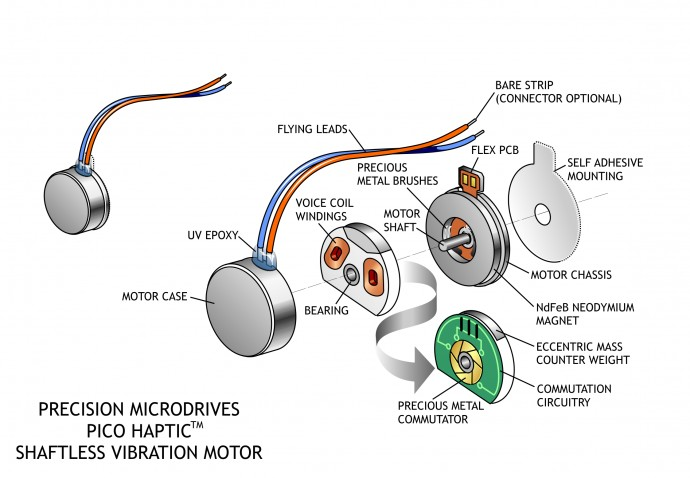
\includegraphics[width=0.7\textwidth]{Pictures/coin_motor.jpg}%imagine location
	\caption{The components of coin vibration motor~\cite{coin_motor}}\label{fig:coin_motor}%use name for ref.
\end{figure}

In this system, as shown in Fig.~\ref{fig:coin_motor_2} 10 mm coin vibration motors that operate at a nominal voltage of 3 V are attached to the fingertip regions of the glove to enhance skin contact and tactile feedback. The motors are controlled using Pulse Width Modulation (PWM) signals generated by the ESP32 microcontroller. By adjusting the PWM duty cycle and frequency, the system can modulate the intensity and frequency of the vibrations, simulating different levels of surface smoothness or roughness in virtual environments.

\begin{figure}[H]\centering
	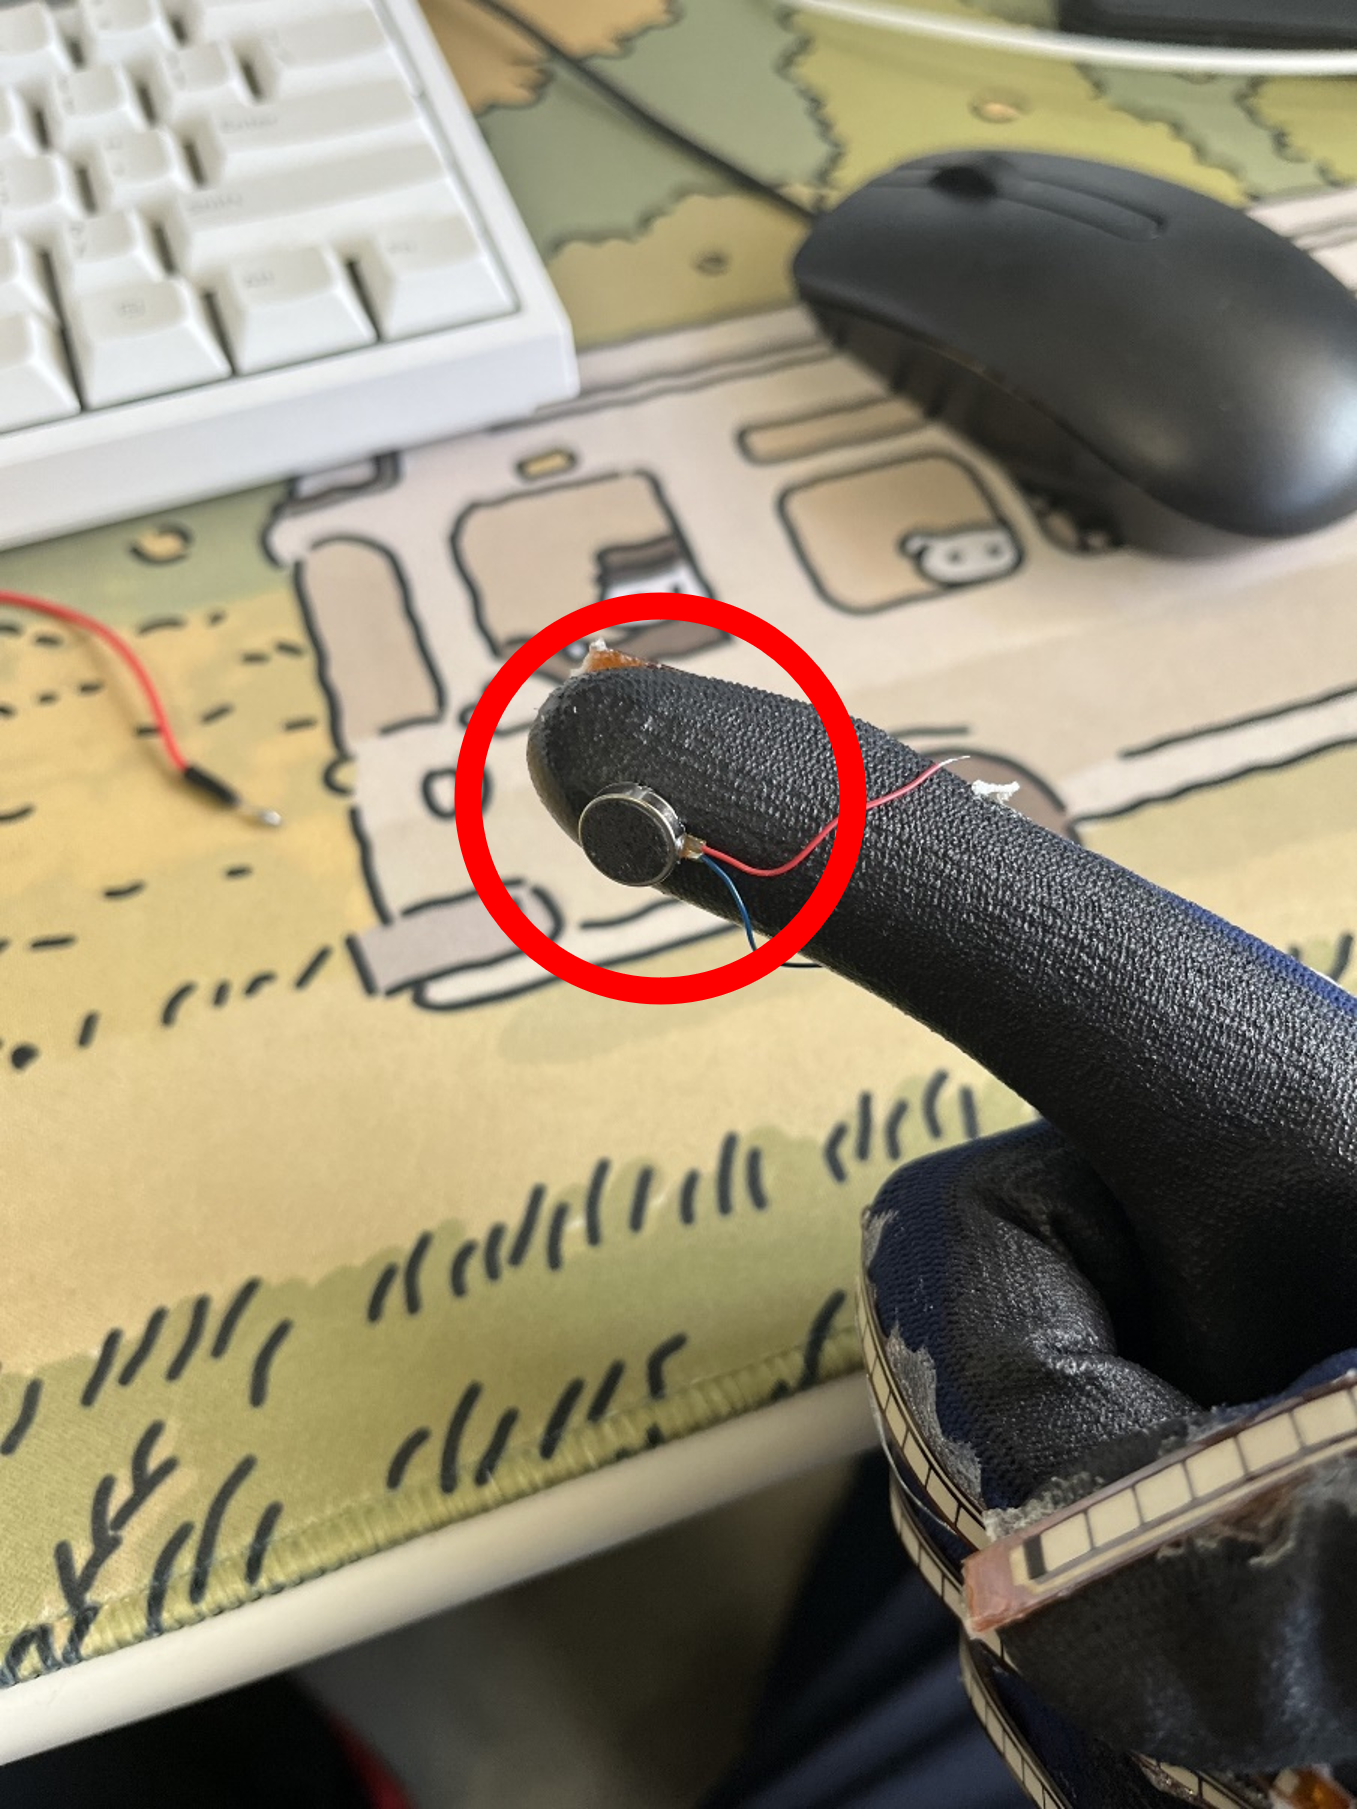
\includegraphics[width=0.5\textwidth]{Pictures/coin_motor_2.png}%imagine location
	\caption{Attached coin motor}\label{fig:coin_motor_2}%use name for ref.
\end{figure}


% This paper proposes a strategy with a time-dependent synced-rotational gain to avoid collisions between multiple VR users sharing the same physical space. A time-dependent synced-rotational gain will rotate the coordinates of all the virtual environments as the time passes, which belong to the users in a collision course in order to have them face in a different direction to avoid collisions. Fig.~\ref{fig:Time-Dependent Synced Rotational Strategy} shows the process of the strategy. Fig.~\ref{fig:Time-Dependent Synced Rotational Strategy_a} predicts a collision from walking directions of three users and their current positions in their physical space. After the collision is predicted, Fig.~\ref{fig:Time-Dependent Synced Rotational Strategy_b} rotates the coordinates of their VR cameras counterclockwise
% at the same time to change their facing direction. Fig.~\ref{fig:Time-Dependent Synced Rotational Strategy_c} shows the result of the strategy.

% This strategy is expected to be better than Holm's method when more than two users sharing the same physical space because when three or more users have predicted a collision at the same time, Holm's method can enable collision avoidance function for just two users. The other user will get nothing, but our method can enable a collision avoidance function when three or more users are predicted a collision.

% \begin{figure}[H]
% 	\centering
% 		\subfigure[Predict a collision.]{
% 			\begin{minipage}[t]{0.5\linewidth}
% 				\centering
% 				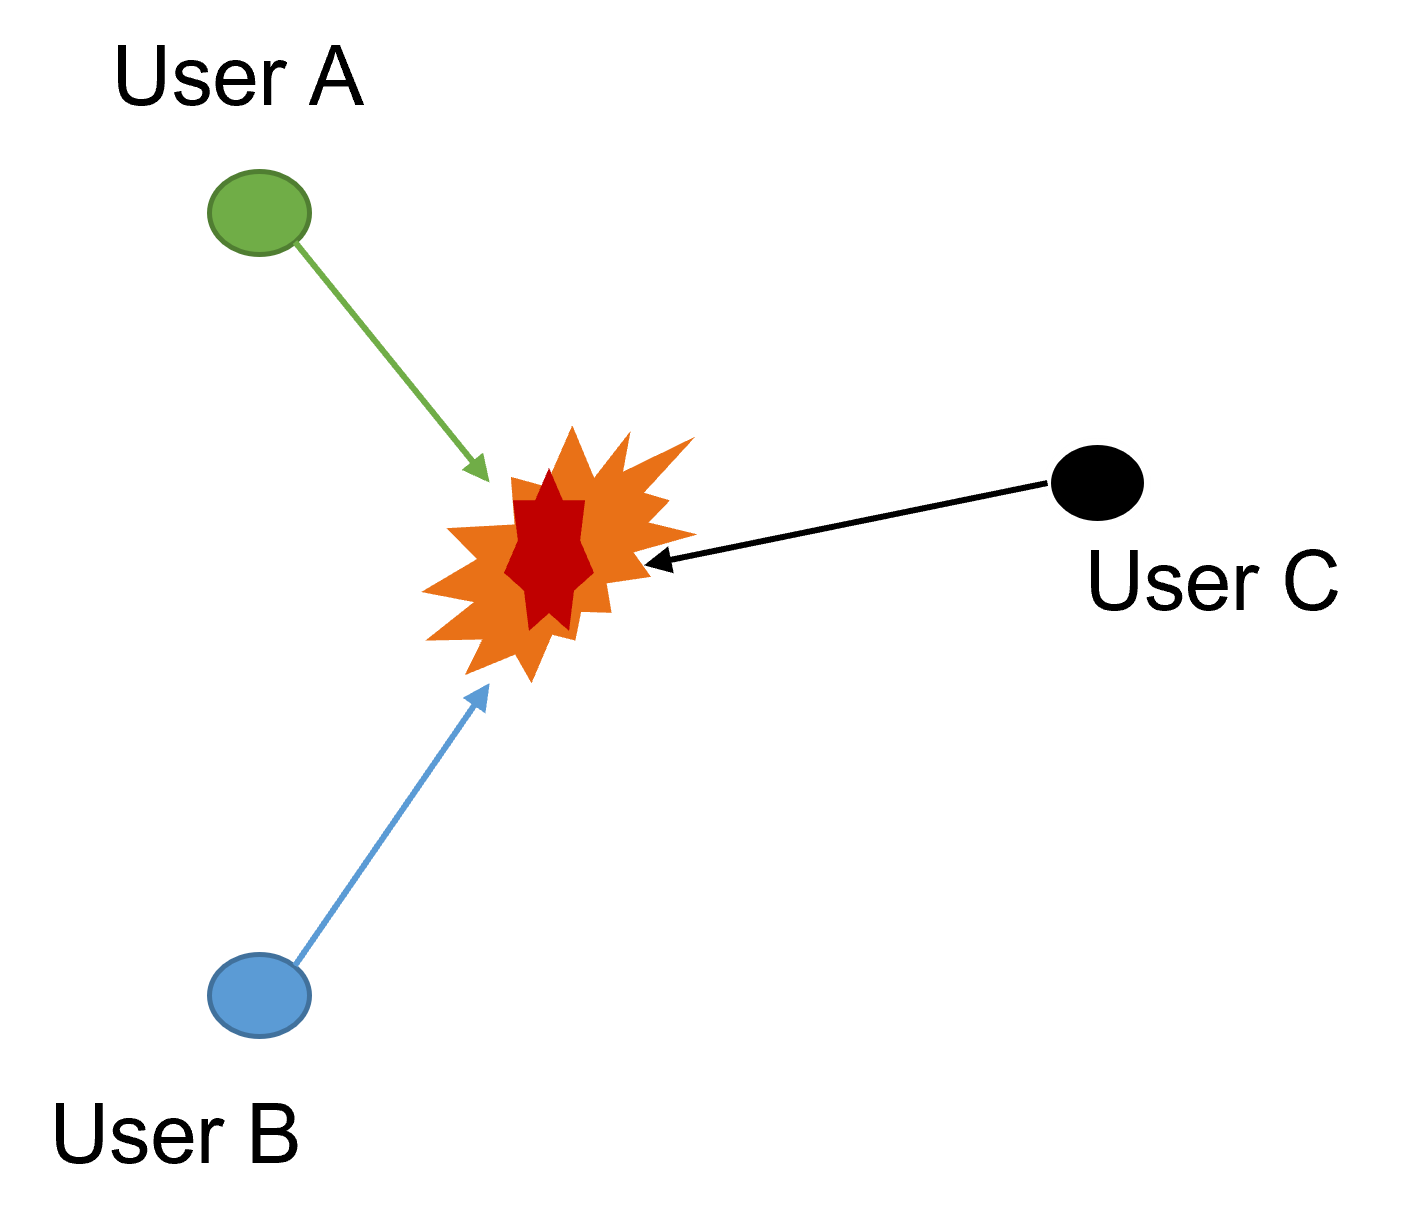
\includegraphics[width=1.9in]{Pictures/A strategy with a time-dependent synced rotational gain_1.png}
% 				\label{fig:Time-Dependent Synced Rotational Strategy_a}
% 			\end{minipage}
% 		}%
% 		\subfigure[Rotate the coordinates of the VR cameras counterclockwise that belong to users on a collision course.]{
% 			\begin{minipage}[t]{0.5\linewidth}
% 				\centering
% 				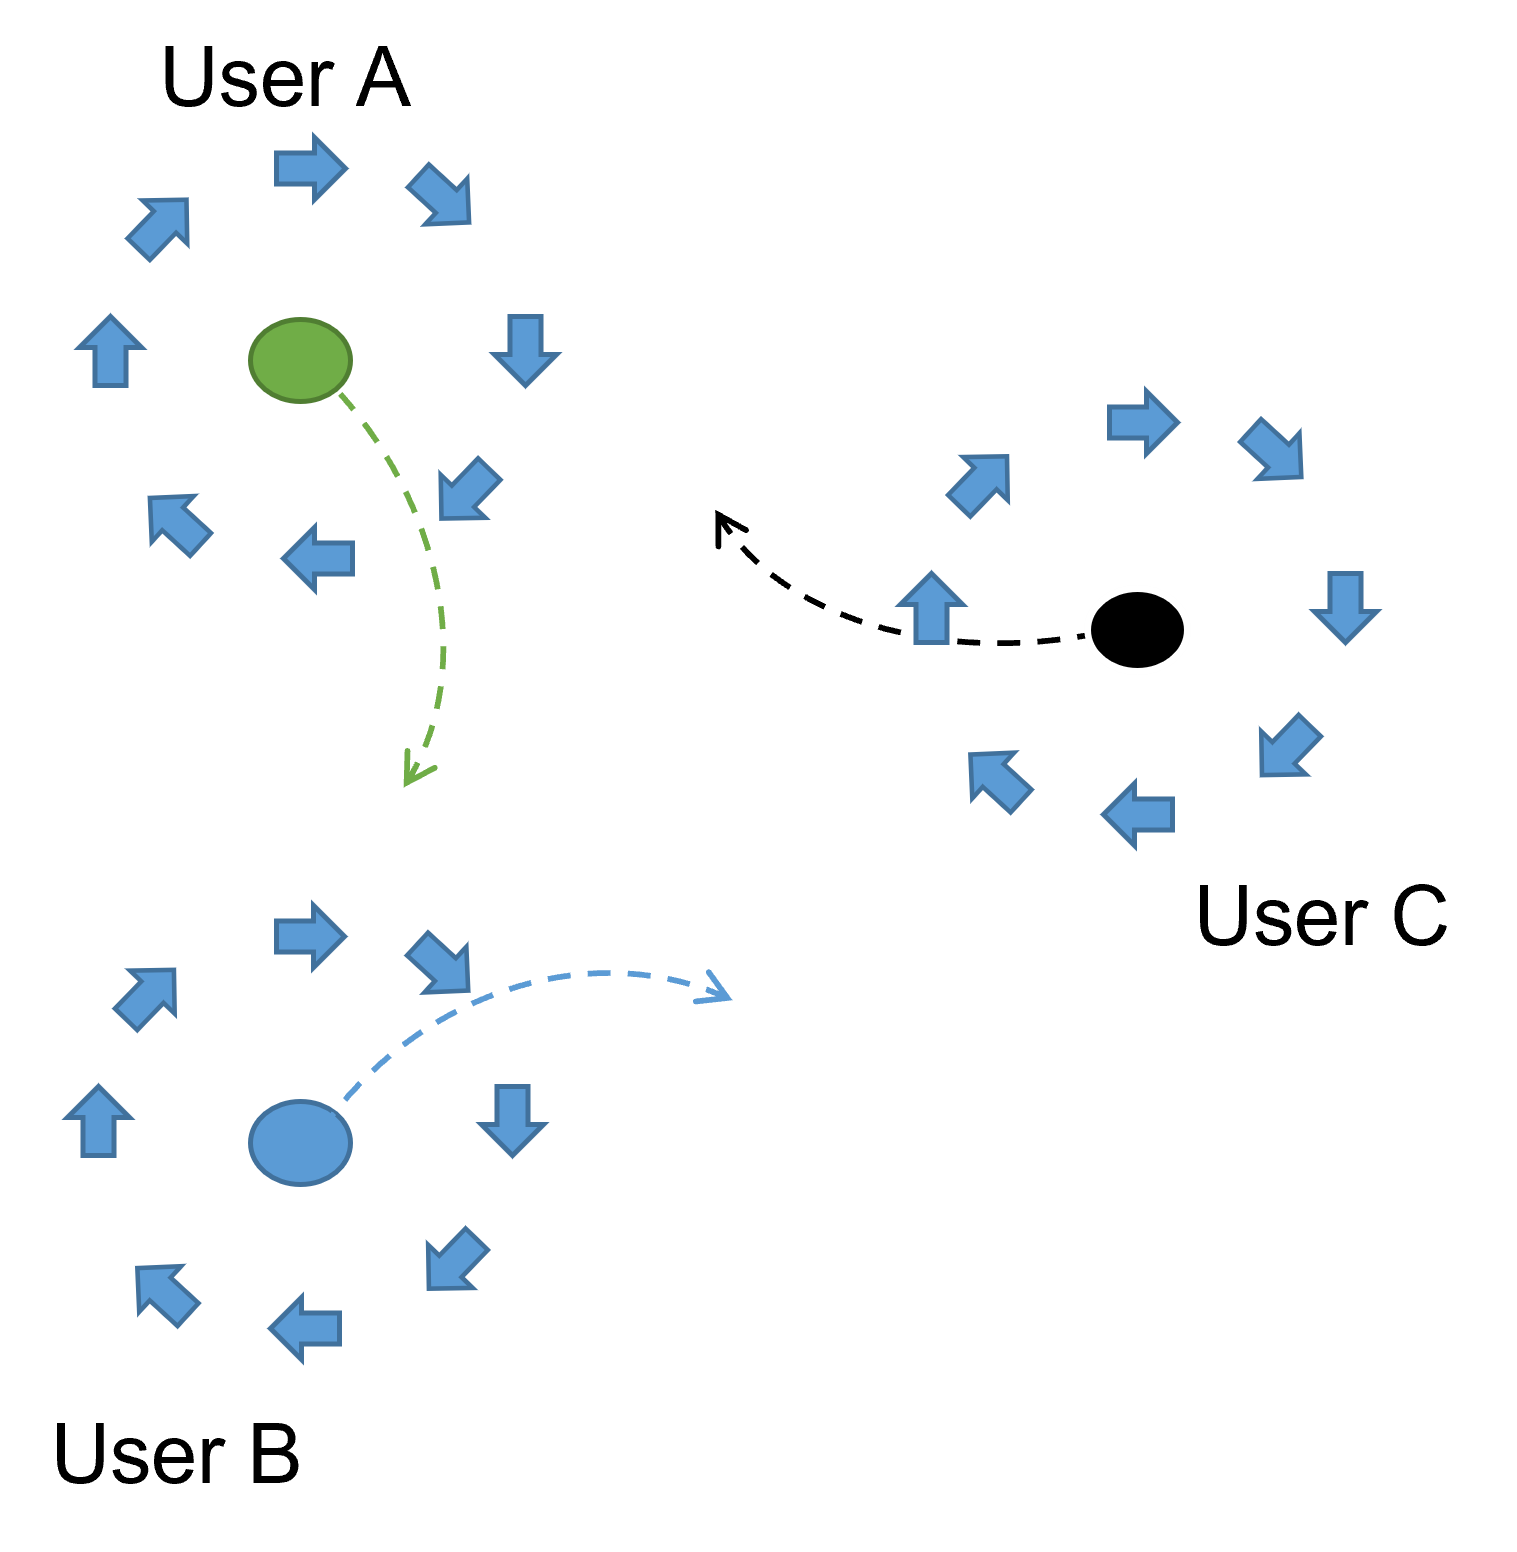
\includegraphics[width=1.9in]{Pictures/A strategy with a time-dependent synced rotational gain_2.png}
% 				\label{fig:Time-Dependent Synced Rotational Strategy_b}
% 			\end{minipage}
% 		}%

% 		\subfigure[Change the users' facing direction at the same time.]{
% 			\begin{minipage}[t]{0.5\linewidth}
% 				\centering
% 				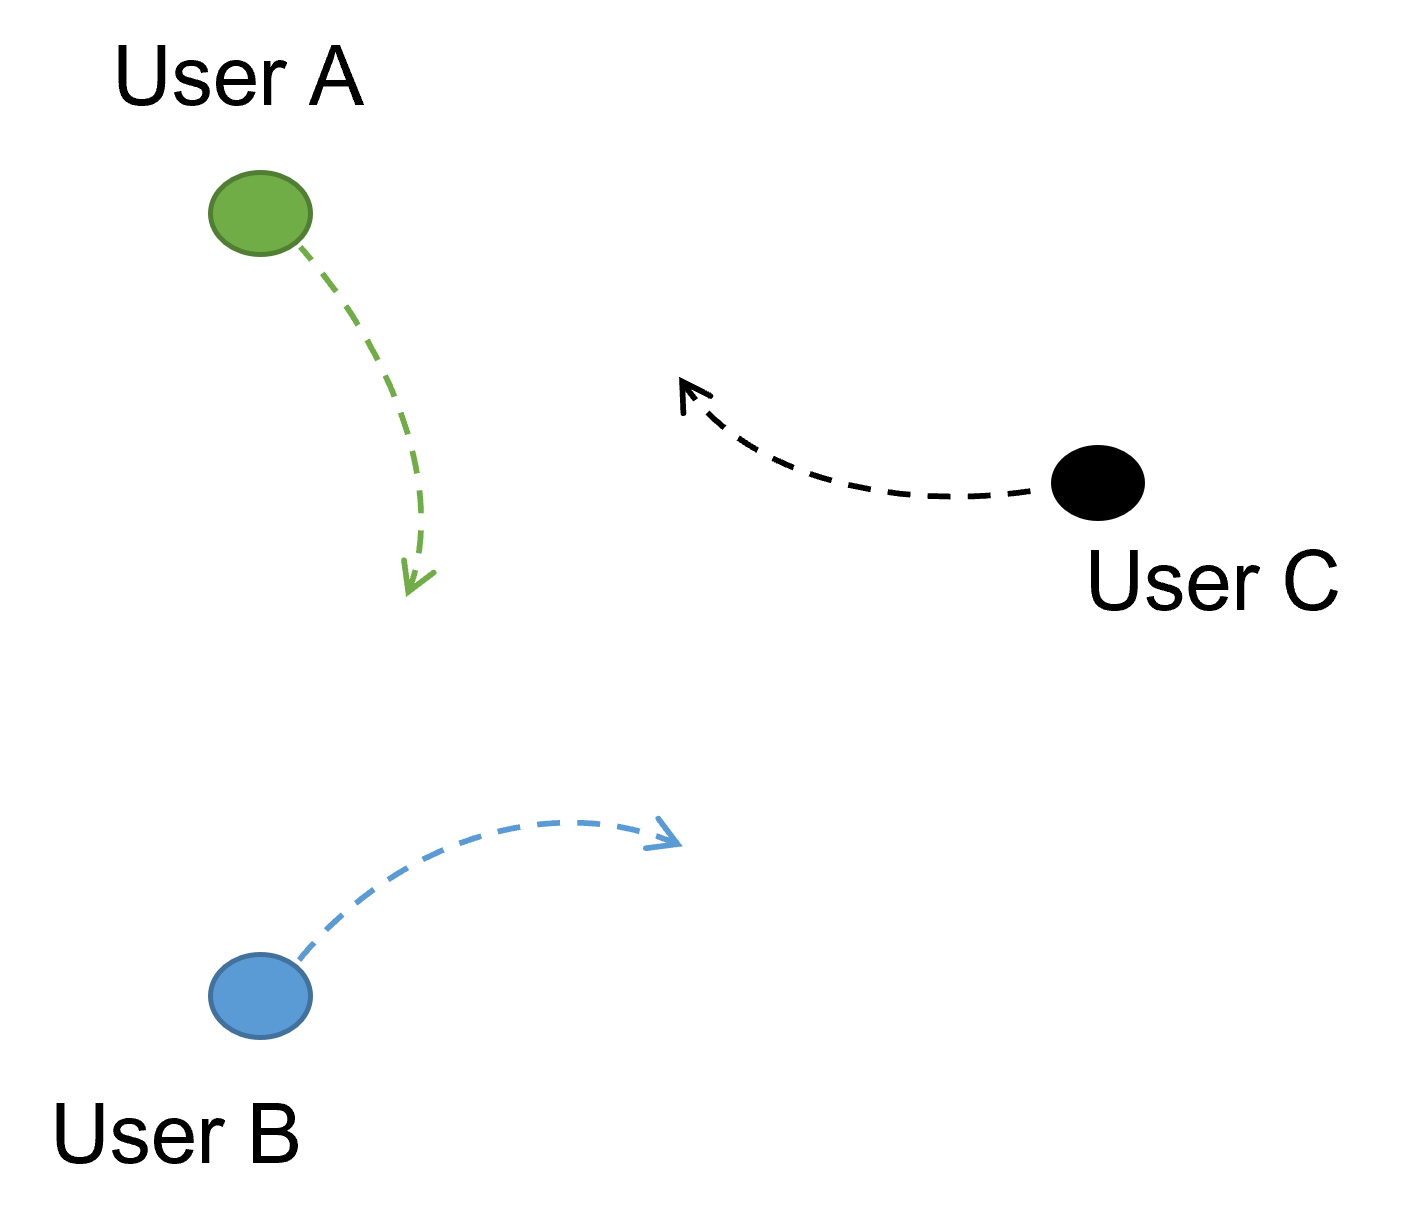
\includegraphics[width=1.9in]{Pictures/A strategy with a time-dependent synced rotational gain_3.png}
% 				\label{fig:Time-Dependent Synced Rotational Strategy_c}
% 			\end{minipage}
% 		}%
	
% 		\centering
% 		\caption{A strategy with a time-dependent synced rotational gain.}
% 		\label{fig:Time-Dependent Synced Rotational Strategy}
% \end{figure}

% To make the proposed method work properly, the following two properties should be figured out prior to implementation.
% \begin{enumerate}
%   \item Sensitivity of rotational awareness of humans in a virtual environment
%   \item Curvature distance of humans walking in a rotating virtual environment
% \end{enumerate}

% %%%%%%%%%%%%%%%%%%%%%%%%%%%%%%%%%%%%%%%%%%%%%%%%%%%%%%%
% %Positon prediction&Walking direction prediction/Collision detection/Collision avoidance
% For predicting a collision of users and detecting the collision, the proposed method implements the position prediction, walking direction prediction and collision detection from the Holm's method mentioned in the previous chapter. As for collision avoidance, the Holm's method is designed to handle between two users. If the number of users is three or more users sharing the same physical space, a collision might occur between more than two users at the same time. In that case, the exceed users from two will get nothing and are not treated as the target of collision avoidance. The proposed method can reduce the collision number when the collision occurs between more than two users.






% %%%%%%%%%%%%%%%%%%%%%%%%%%%%%%%%%%%%%%%%%%%%%%%%%%%%%%%
% \newpage
% %%%%%%%%%%%%%%%%%%%%%%%%%%%%%%%%%%%%%%%%%%%%%%%%%%%%%%%%%%
% %%%%%%%%%%%%%%%%%%%%%%%%%%%%%%%%%%%%%%%%%%%%%%%%%%%%%%%%%%	
% \section{Sensitivity of rotational awareness of humans in a virtual environment}
% For properties of rotation of a virtual environment, the purpose of this experiment is to figure out the threshold that humans cannot sense the applied rotation.


% \subsection{Experiment tasks}
% In this experiment, three tasks are employed: stop to constant speed rotation task, constant speed to stop rotation task, deceleration rotation task and acceleration rotation task. 

% Fig.~\ref{fig:topView} and Fig.~\ref{fig:sideView} represent a virtual environment used in the experiment. At the beginning of tasks, the position of a user is located at the origin (0,0) on XZ plane. In the figures, the user stands at the origin. The user can see around in the virtual environment from a field of view of 110 degrees (Fig.~\ref{fig:sideView}), and the user can freely turn around in the virtual environment. 


% \begin{figure}[H]\centering
% 	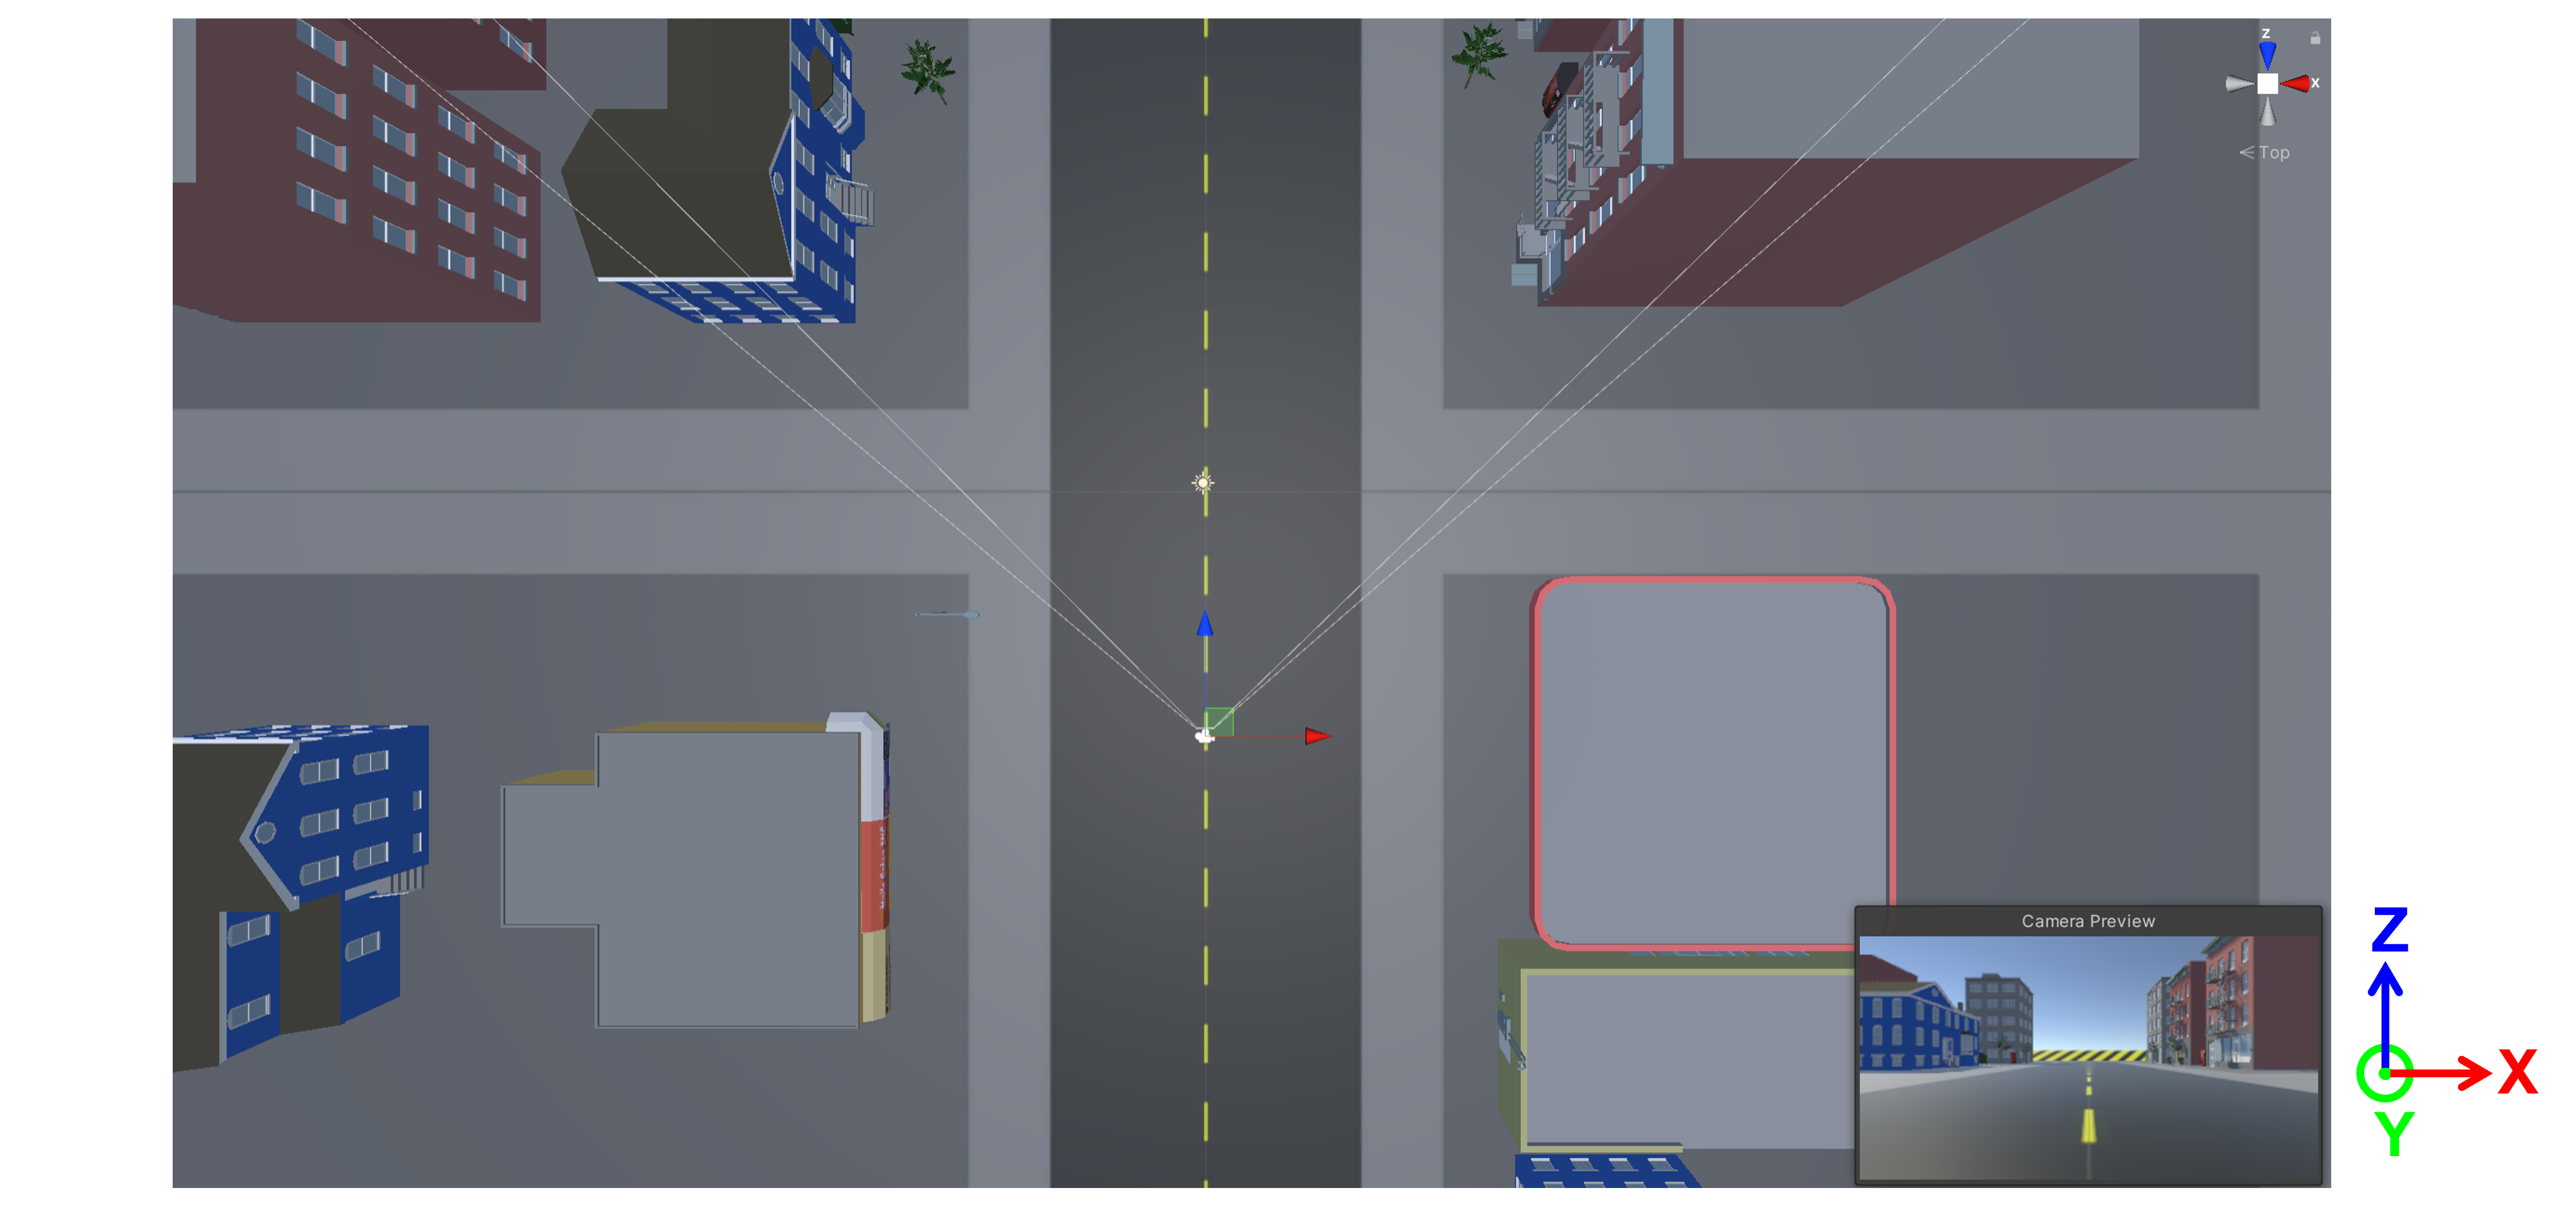
\includegraphics[width=0.95\textwidth]{Pictures/topView.png}%imagine location
% 	\caption{A virtual environment from top view.}\label{fig:topView}%use name for ref.
% \end{figure}

% \begin{figure}[H]\centering
% 	\includegraphics[width=1.1\textwidth]{Pictures/siteView.png}%imagine location
% 	\caption{A virtual environment from side view.}\label{fig:sideView}%use name for ref.
% \end{figure}
% \newpage

% To realize a visual effect of rotating a virtual environment, relative rotation is applied to a virtual camera of the user, independently of his/her own rotation.

% The stop to constant speed rotation task examines degree of sensitivity of humans' rotational awareness for a sudden start to the given speed. The subject puts on an HMD, then a randomly selected rotation speed (0.4deg/s, 0.8deg/s, 1.6deg/s, 3.2deg/s, 6.4deg/s and 12.8deg/s) is applied to the HMD coordinates. The subject is asked to press the button when he/she becomes aware of the rotation and the elapsed time is recorded. After that, the randomly selected speed for next is applied and the procedure is repeated.

% \begin{figure}[H]\centering
% 	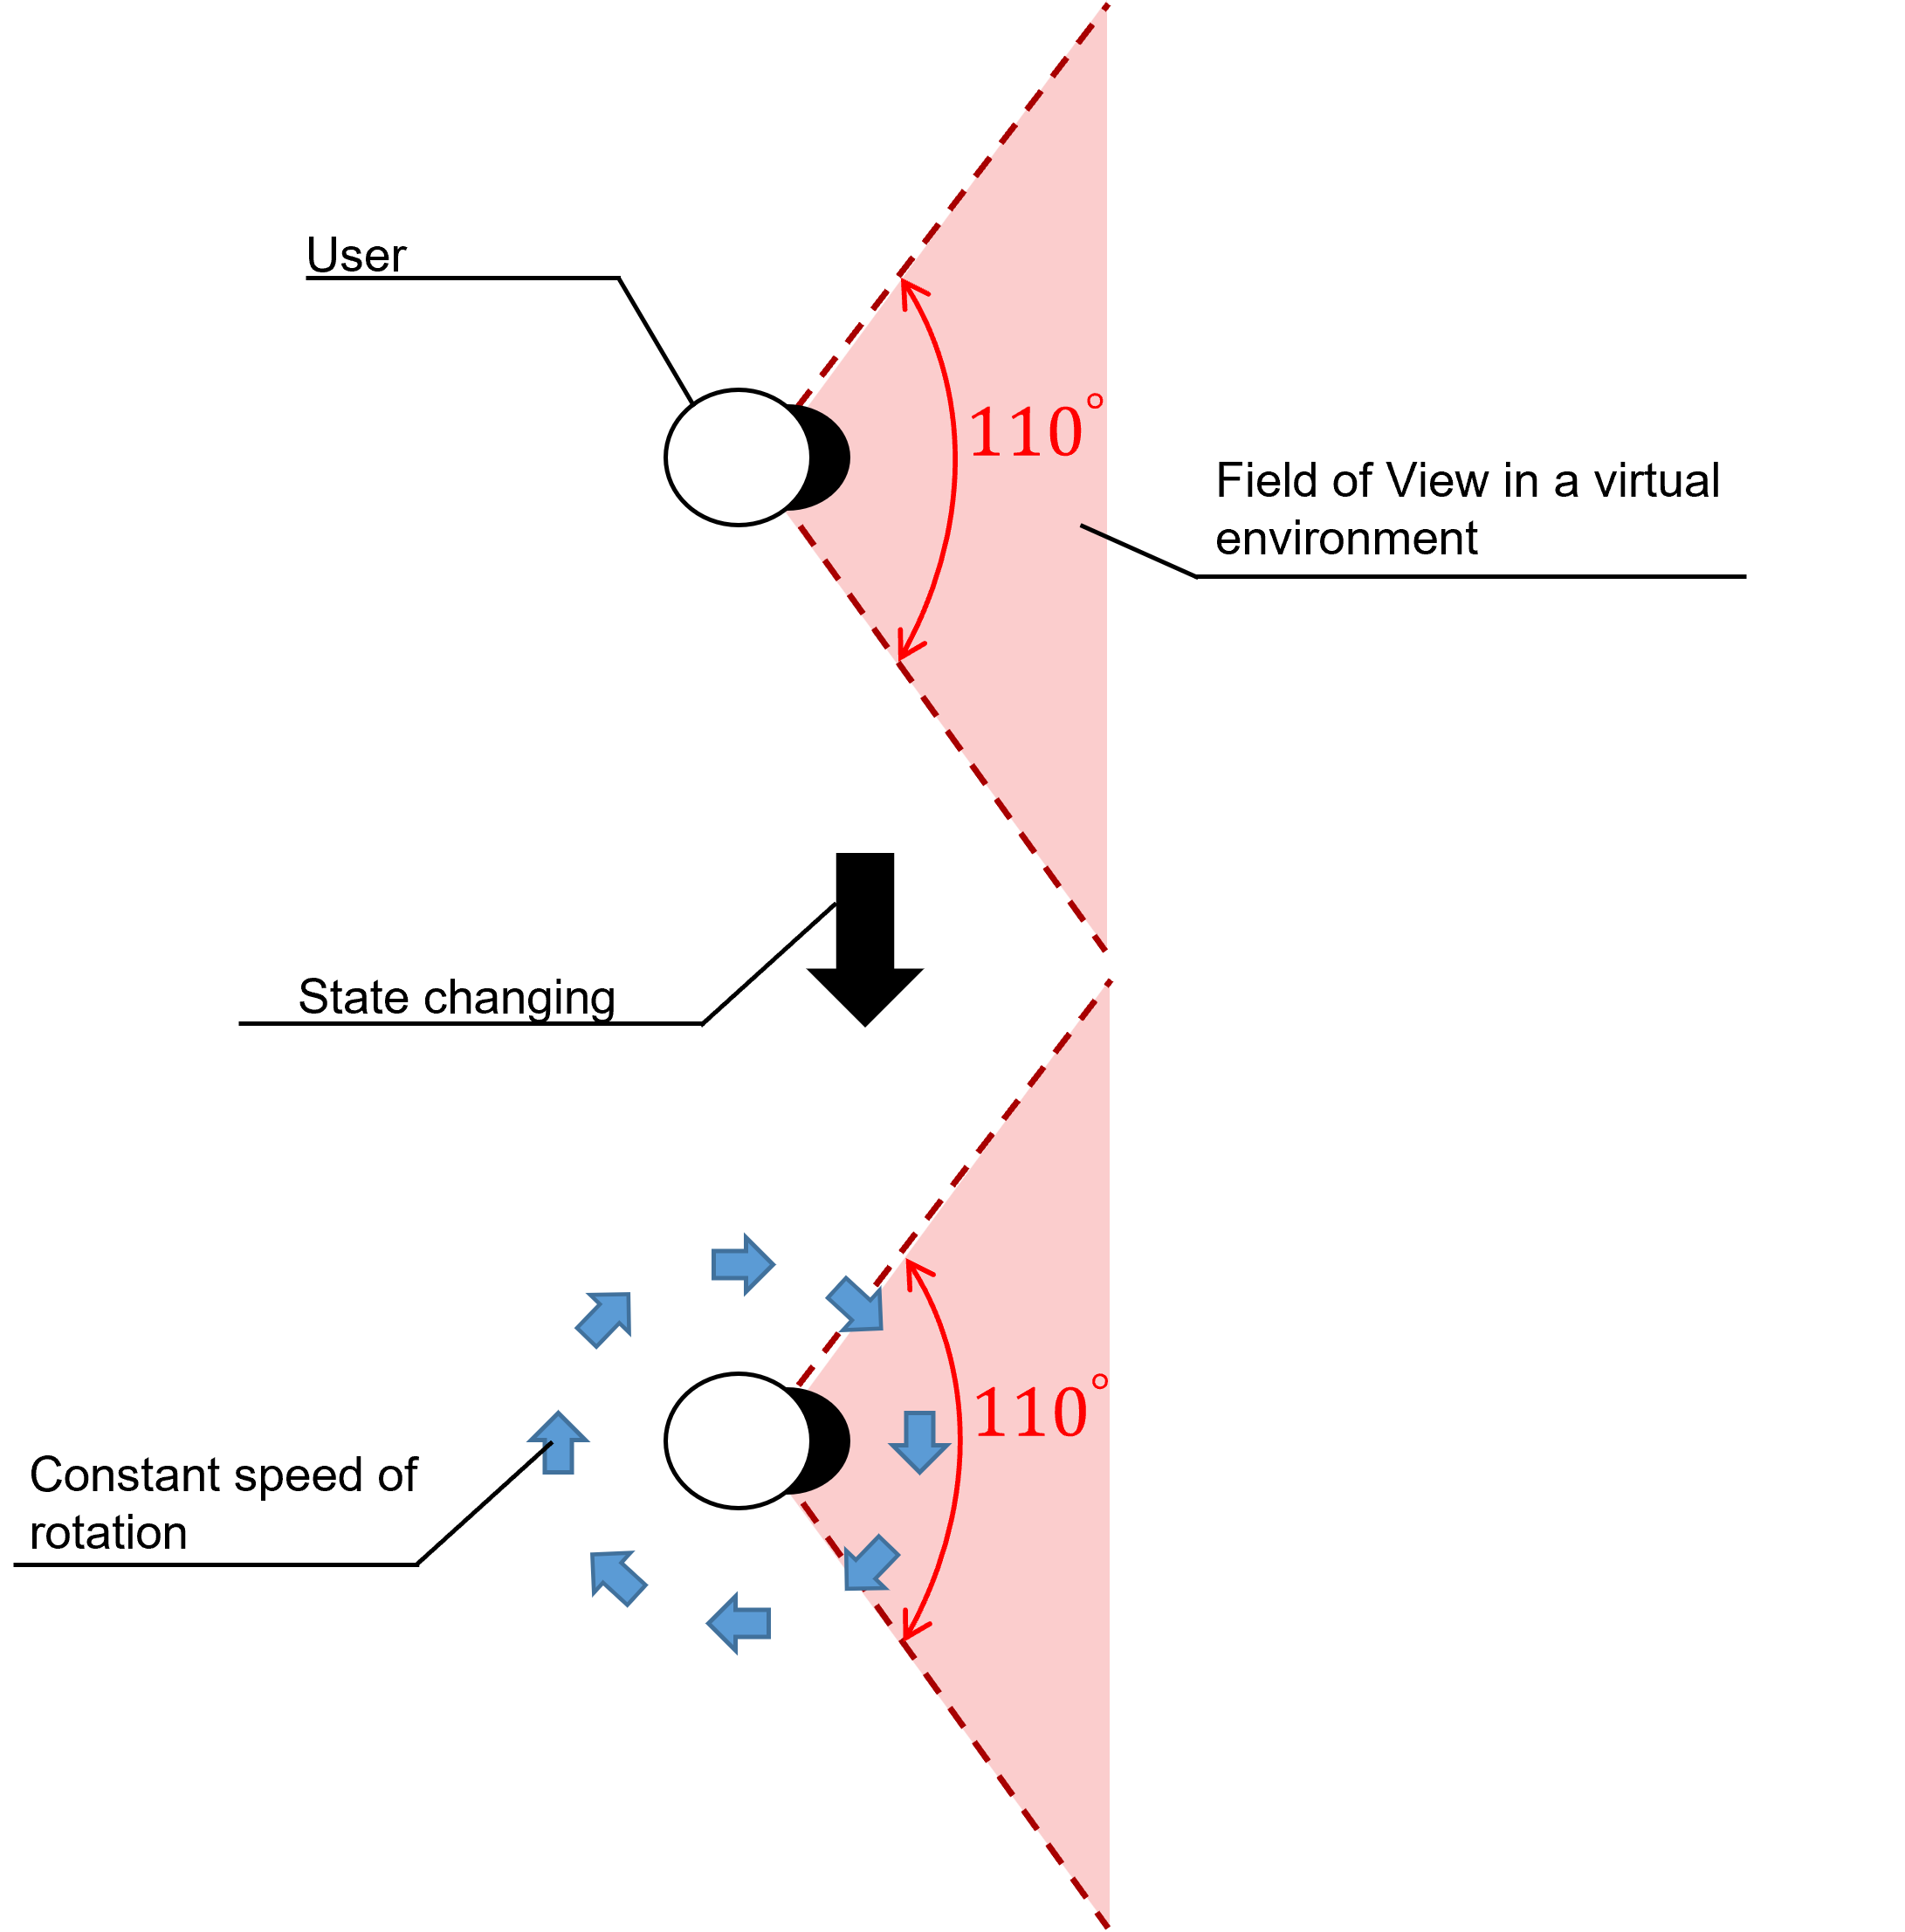
\includegraphics[width=1.0\textwidth]{Pictures/Equipment 1 Constant Speed task.png}%imagine location
% 	\caption{Stop to constant speed rotation task.}\label{fig:Equipment 1 Constant Speed task}%use name for ref.
% \end{figure}
% \newpage
% %%%%%%%%%%%%%%%%%%%

% The constant speed to stop rotation task examines degree of sensitivity of humans' rotational awareness for a sudden stop from given constant rotation speed. The subject puts on an HMD, HMD coordinates are then the rotated by a randomly selected constant speed (0.4deg/s, 0.8deg/s, 1.6deg/s, 3.2deg/s, 6.4deg/s and 12.8deg/s) at the beginning. This rotation stops without notice to the subject. The subject is asked to press the button when he/she becomes aware of the changing and the elapsed time is recorded. After that, the randomly selected speed for next is applied and the procedure is repeated.

% In stop to constant speed and constant speed to stop rotation tasks, the direction of rotation is clockwise.

% %%%%%%%%%%%%%%%%%%
% \begin{figure}[H]\centering
% 	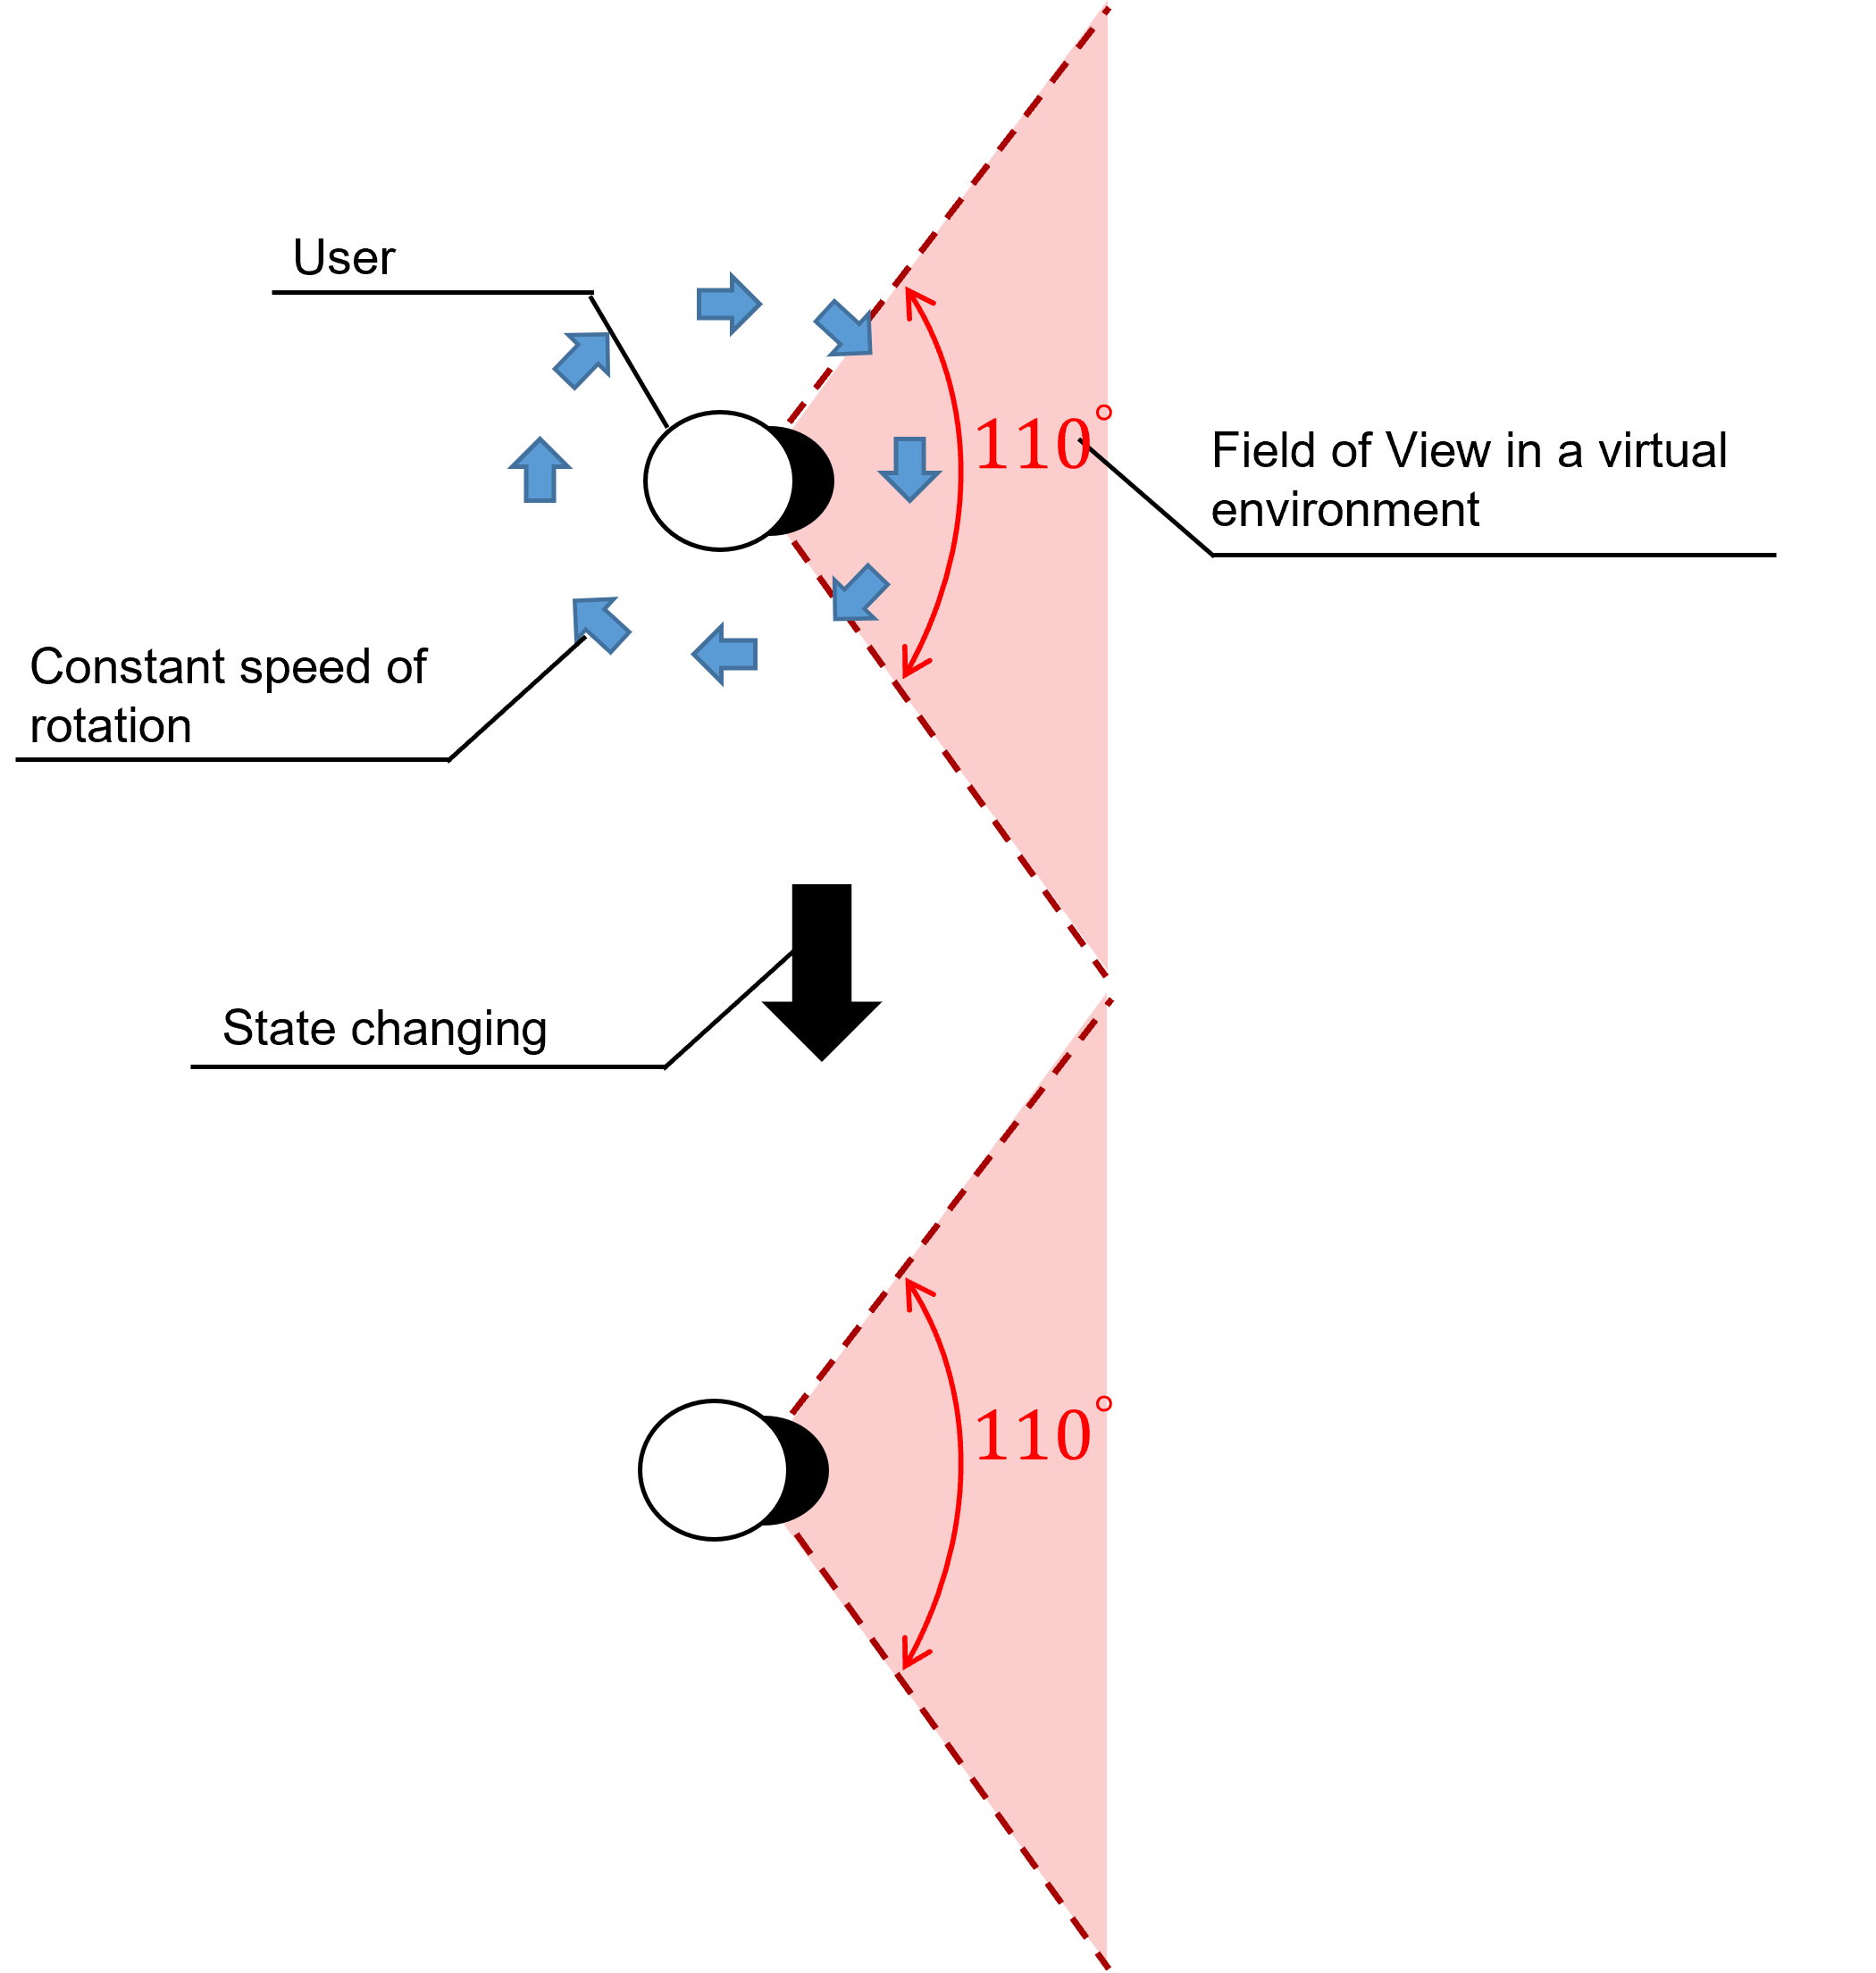
\includegraphics[width=1.0\textwidth]{Pictures/ConstantToStop.png}%imagine location
% 	\caption{Constant speed to stop rotation task.}\label{fig:Constant Speed to Stop Rotation task task}%use name for ref.
% \end{figure}
% \newpage


% The deceleration rotation task examines degree of sensitivity of humans' awareness for a gradual change in speed of rotation. In this task, the HMD coordinates are rotated at the given constant speed (0.4deg/s, 0.8deg/s, 1.6deg/s and 3.2deg/s) when starting. And that speed is gradually decreased by a randomly selected deceleration (33\%, 66\% and 100\%). The $x$\% deceleration means that $x$\% of the given constant speed decreases per second until the speed reaches zero. The subject is asked to press the button when he/she becomes aware of the decrease in rotation speed and the elapsed time is recorded. After that, the randomly selected combination, speed and deceleration, is applied for next and procedure is repeated

% Note that from the constant speed tasks, rotation speeds of 6.4deg/s and 12.8deg/s are high rotation speeds, so that the subjects suddenly responded after enabling or disabling rotation. For the deceleration and acceleration tasks, these speeds are excluded.

% \begin{figure}[H]\centering
% 	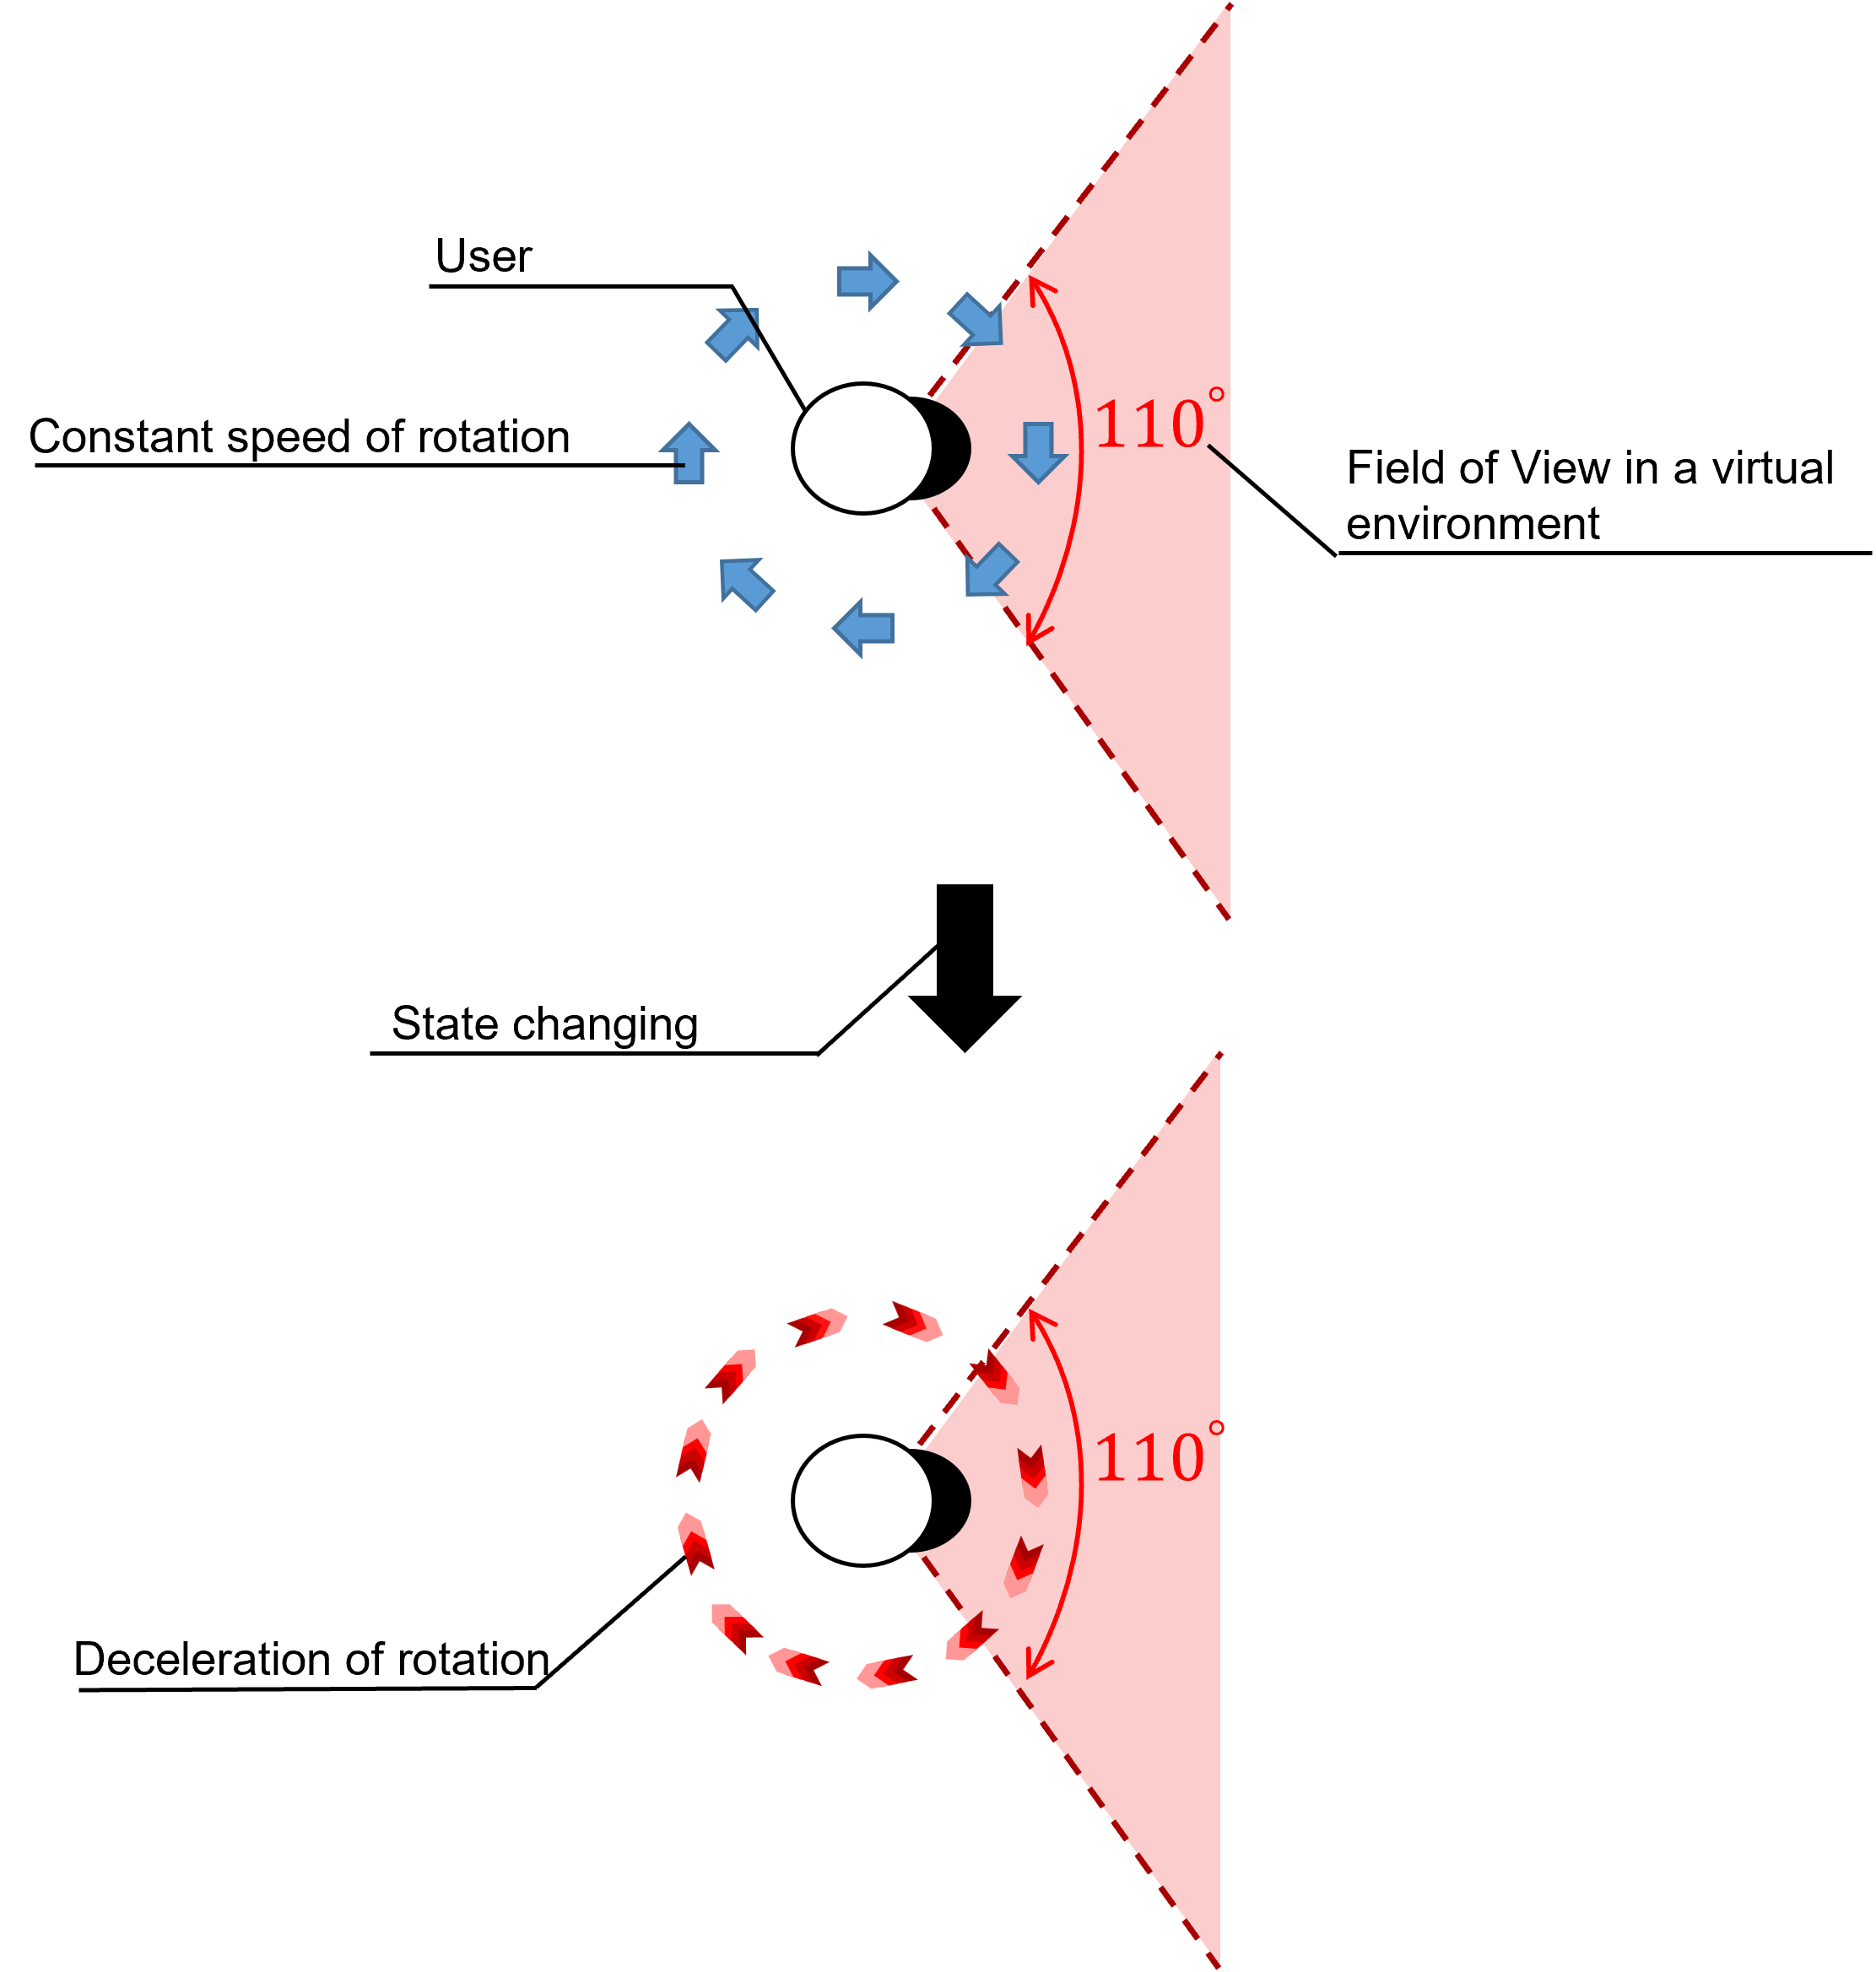
\includegraphics[width=1.0\textwidth]{Pictures/Deceleration Task.png}%imagine location
% 	\caption{Deceleration rotation task.}\label{fig:Equipment 1 Deceleration Task}%use name for ref.
% \end{figure}

% \newpage
% The acceleration rotation task examines degree of sensitivity of humans' awareness for a gradual increase in speed of rotation.
% The initial rotation speed is zero, and a randomly selected rotation speed (0.4deg/s, 0.8deg/s, 1.6deg/s and 3.2deg/s) and a randomly selected acceleration (33\%, 66\% and 100\%) are applied to the HMD coordinates. Here, acceleration of $x$\% indicates that rotation speed increases by $x$\% of the given constant speed per second from zero until the speed reaches it. The subject is asked to press the button when he/she becomes aware of the rotation and the elapsed time is recorded. After that, the randomly selected combination, speed and acceleration, is applied for next and the procedure is repeated.

% In deceleration and acceleration rotation tasks, the direction of rotation is clockwise. Fig.~\ref{fig:Equipment 1 Deceleration Task}, the blue arrow is a constant speed. The red arrow is deceleration rotation, and the arrow color is fading from dark red to bright red, which means the rotation speed decreases to zero. Fig.~\ref{fig:Equipment 1 Acceleration Task} shows the acceleration rotation task. The rotation speed is increasing, shown by fading color from bright red to dark red of the red arrow.

% \begin{figure}[H]\centering
% 	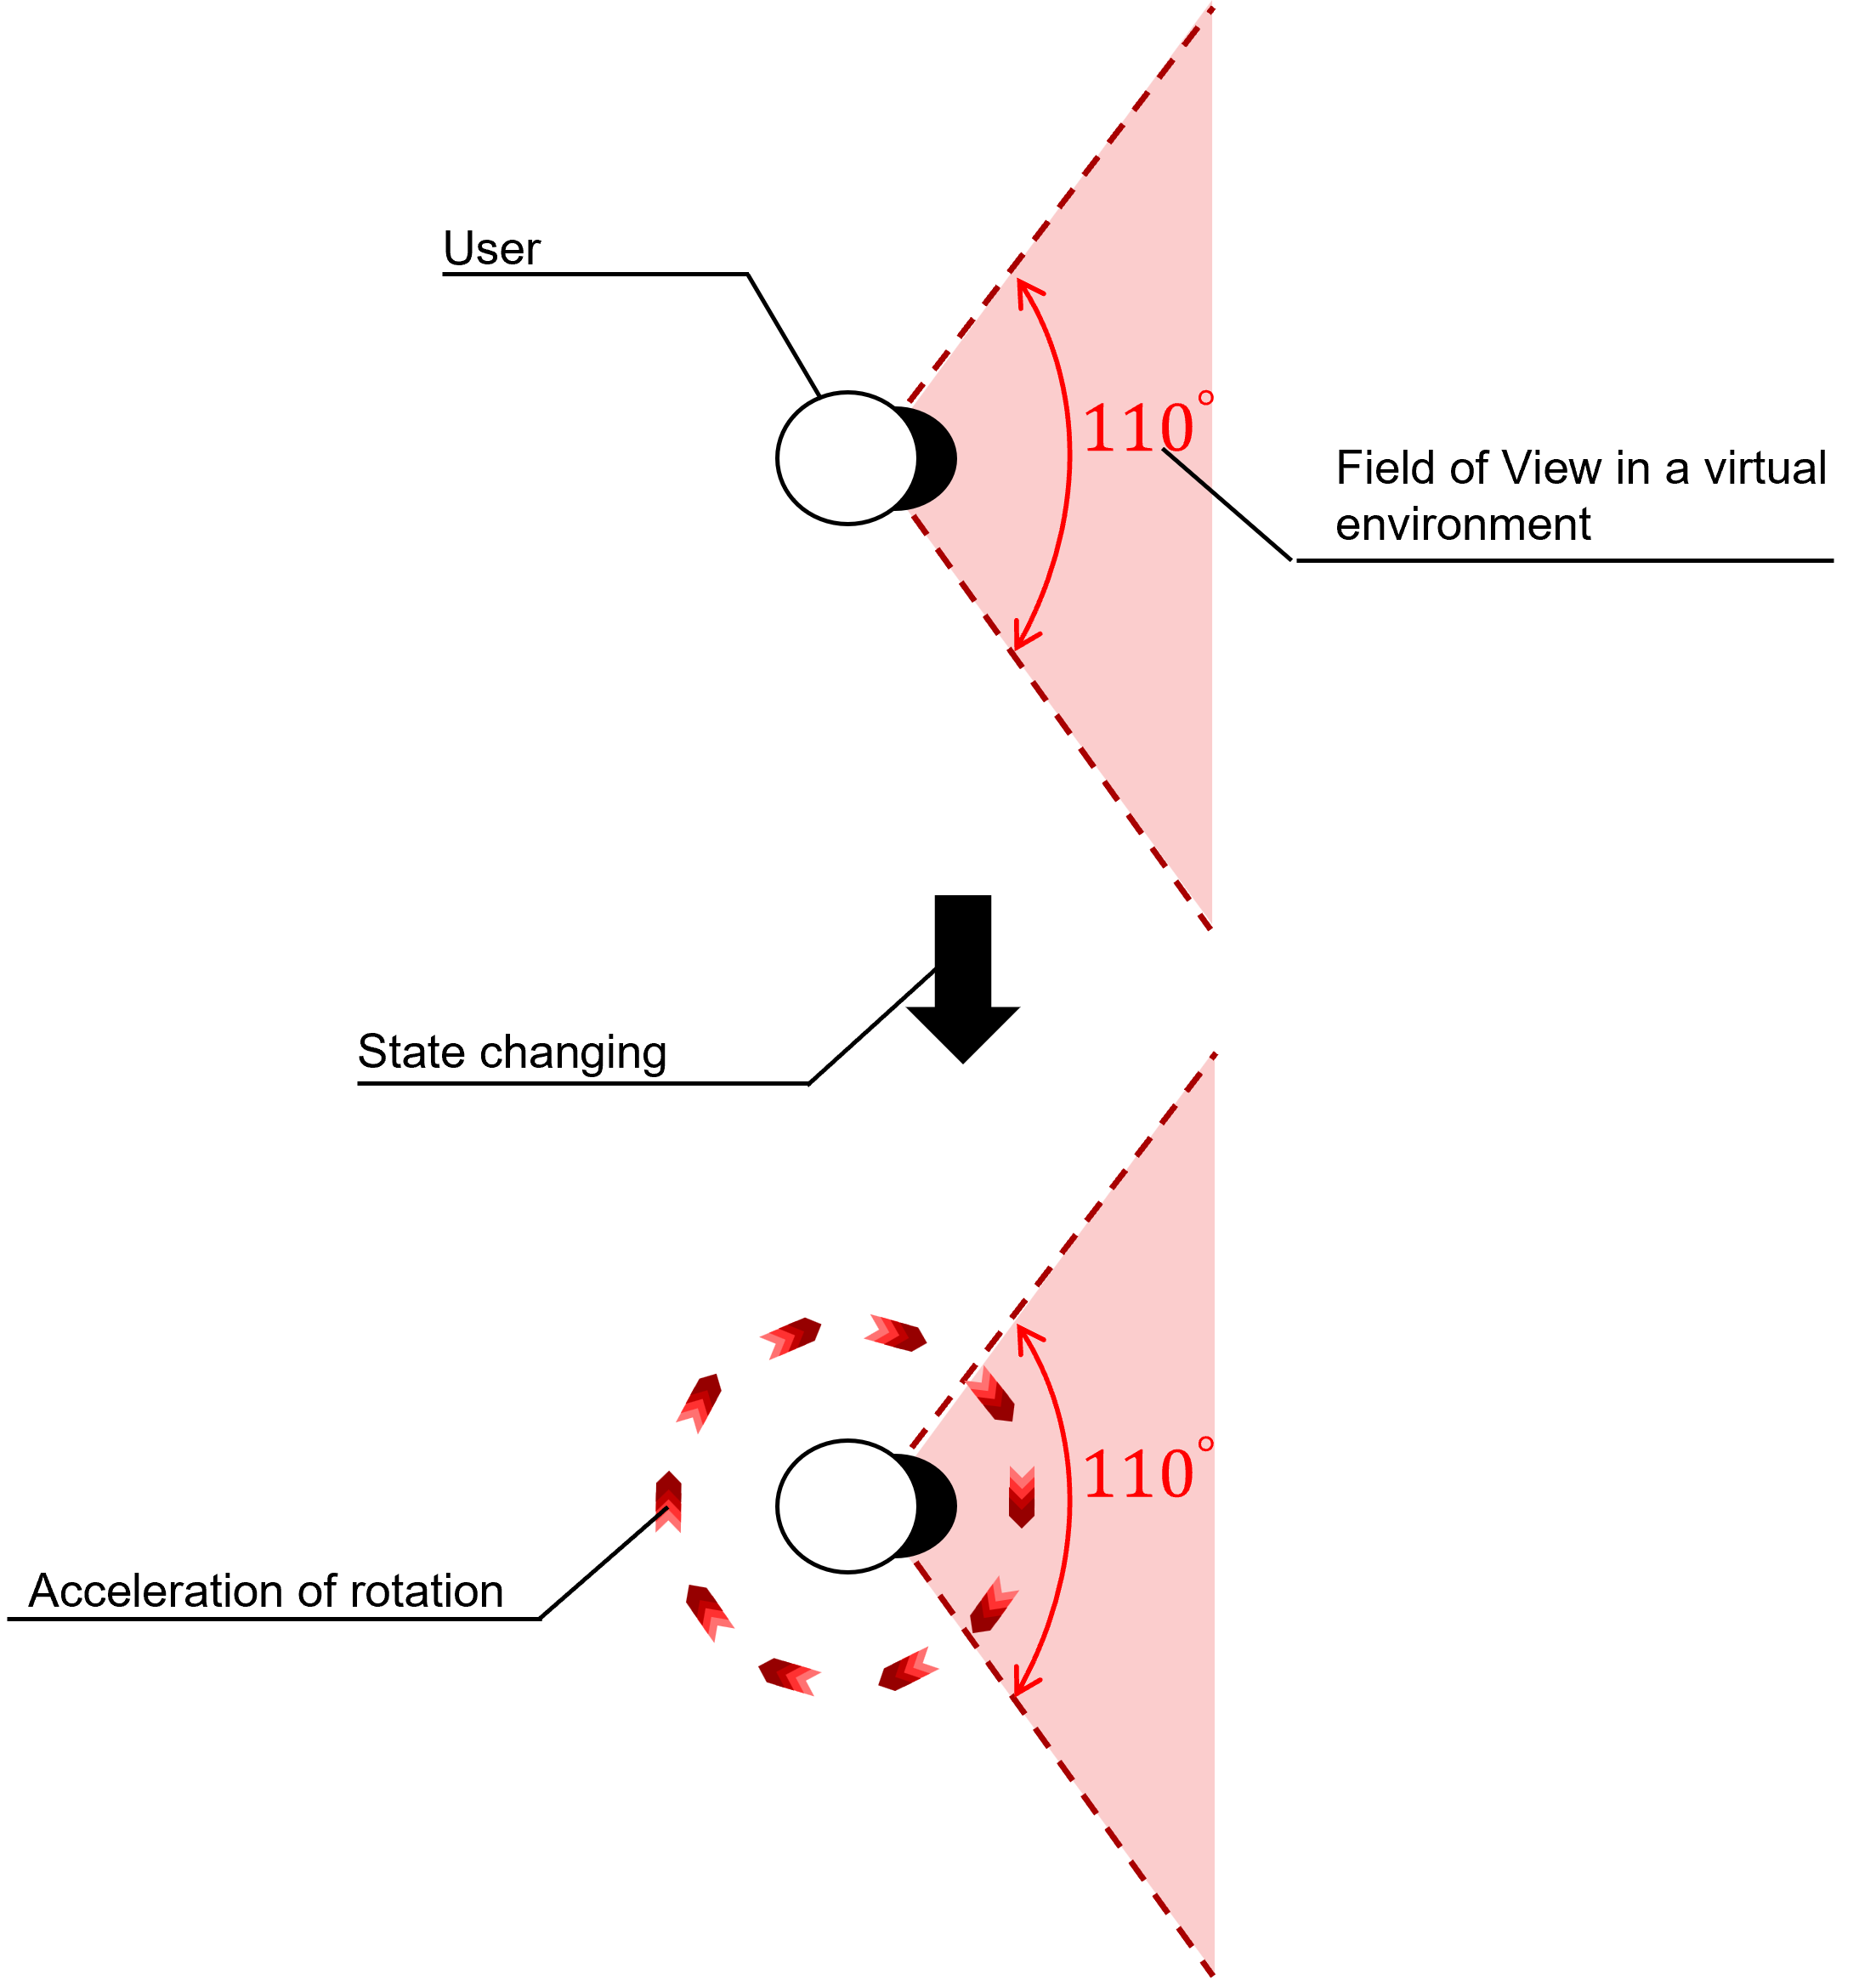
\includegraphics[width=0.9\textwidth]{Pictures/Equipment 1 Acceleration Task.png}%imagine location
% 	\caption{Acceleration rotation task.}\label{fig:Equipment 1 Acceleration Task}%use name for ref.
% \end{figure}
% \newpage
% \subsection{Procedure} 
% Five subjects with the ages of 25 to 27 years old take part in the experiment.
% \begin{enumerate}
% 	\item Each subject wears an HMD.
% 	\item A rotation speed (0.4deg/s, 0.8deg/s, 1.6deg/s, 3.2deg/s, 6.4deg/s and 12.8deg/s) and a percentage of acceleration or deceleration (33\%,66\% and 100\%) are randomly selected.
% 	\item The participant performs the given task (The first task is the stop to constant speed rotation task. The second task is the constant speed to stop rotation task, the third task is the deceleration rotation task and the final task performs the acceleration rotation task. Each task is performed on a different day.).
% 	\item Repeat from step 2 to step 3 at ((6 speeds x 3 trials x 2 tasks) + (4 speeds x 3 percentages x 3 trials x 2 tasks) = 108 trials)
% \end{enumerate}

% The subjects can take a break every 5 minutes to check VR motion sickness symptoms as shown in Fig.~\ref{fig:Virtual reality sickness questionnaire_1}.
% \begin{figure}[H]\centering
% 	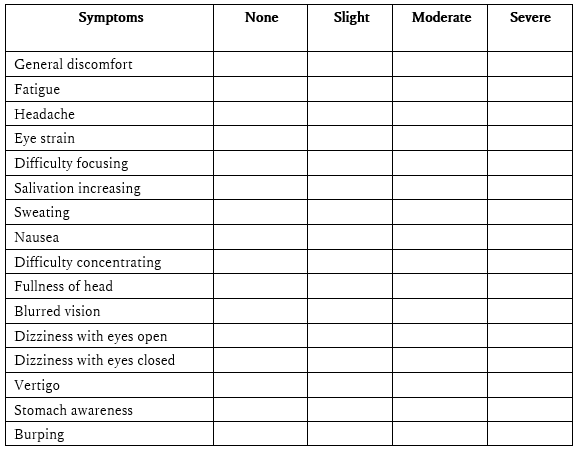
\includegraphics[width=1.0\textwidth]{Pictures/Virtual reality sickness questionnaire.png}%imagine location
% 	\caption{Virtual reality sickness questionnaire~\cite{Norman2018EvaluationOV}.}\label{fig:Virtual reality sickness questionnaire_1}%use name for ref.
% \end{figure}
% \newpage
% \subsection{Data collection}
% For each task, the following data is collected.

% \begin{table}[h!]\centering
% 	\caption{Data collection.}
% 	\label{tab:Data CollectionEx1}%\scriptsize
% 		\scalebox{1.0}{
% 	\begin{tabular}{ |p{4cm}|p{3cm}|p{6cm}|}
% 	\hline
% 		Variable & Unit & Description \\\hline
% 		Elapsed time & second & Time to be aware.\\\hline
% 		Rotation speed & deg/second & Rotation speed of the coordinates of an HMD.\\\hline
% 		Acceleration (for acceleration rotation task) or deceleration (for deceleration rotation task) & percentage & Degree of accelerate or deceleration of the rotation speed.\\\hline
		
% 	\end{tabular}
% 	}
% \end{table} 

% Independent variables are Rotation speed and Acceleration or deceleration while a dependent one is Elapsed time.
% \newpage
% \subsection{Equipment}
% The experiment system is developed on the Unity platform. The version of Unity is 2019.4.17f1. In terms of hardware, an HMD is served by HTC VIVE Cosmos (Fig.~\ref{fig:EquipmentAndSpecification}), which has a resolution of 1080x1200 pixels per eye, a diagonal field of view of roughly 110 degrees, and a frame rate of 90Hz. Two base stations included with HTC Vive are used for positional tracking, shown in Fig.~\ref{fig:Equipment1_AndSpecification}.

% The HMD is connected to a computer with a CPU of Core i7 (8 cores), a GPU of NVIDIA GeForce GTX 1650 Super and a memory of 16GB.
% \begin{figure}[H]\centering
% 	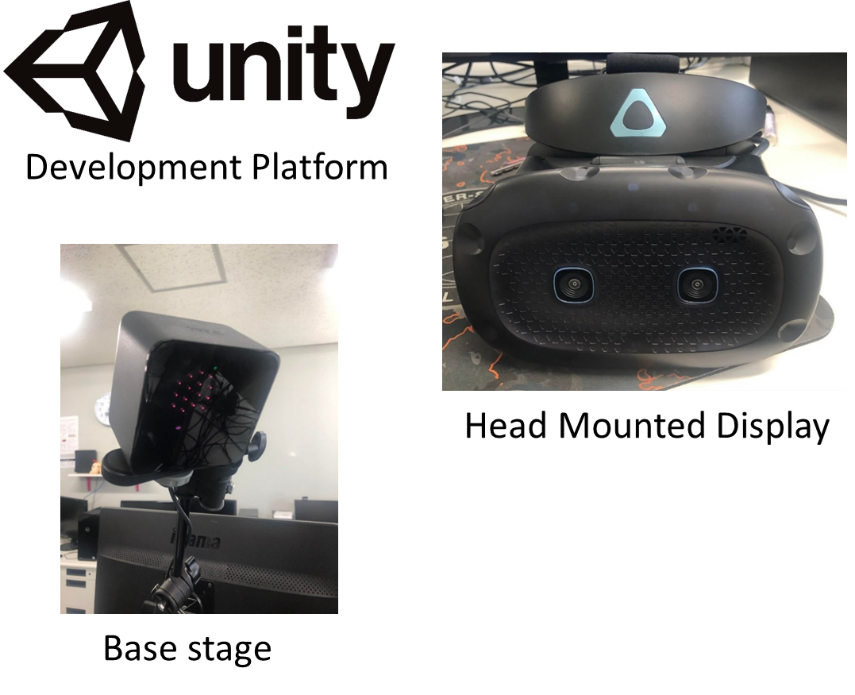
\includegraphics[width=0.6\textwidth]{Pictures/EquipmentAndSpecification.png}%imagine location
% 	\caption{Equipment and specification.}\label{fig:EquipmentAndSpecification}%use name for ref.
% \end{figure}
% \begin{figure}[H]\centering
% 	\includegraphics[width=1.2\textwidth]{Pictures/Experiment1_Overview.png}%imagine location
% 	\caption{A scene of the experiment.}\label{fig:Equipment1_AndSpecification}%use name for ref.
% \end{figure}
% \newpage
% \subsection{Results}
% Fig.~\ref{fig:Six constant speeds} shows a relationship between constant rotation speeds and the elapsed time to notice for the stop to constant speed rotation task. From the figure, when a rotation speed is slower than 0.8deg/s, it will take 10s for users to notice.

% Fig.~\ref{fig:Stop to Six constant speeds} shows a relationship between constant rotation speeds and the elapsed time to notice for the constant speed to stop rotation task. From the result, a rotation speed is 0.4deg/s, the average elapsed time to notice is 7.72s.

% Fig.~\ref{fig:Three deceleration of rotation} shows the impact of deceleration in rotation speed on the elapsed time. As the level of deceleration becomes smaller, it will take more time for users to notice. When a percentage of 33\%, subjects are going to take a long time to notice the rotation. The average elapsed time to notice at 33\% are 9.48s, 4.388s, 3.578s and 1.942s for the max rotation speed of 0.4deg/s, 0.8ged/s, 1.6deg/s and 3.2deg/s, respectively.

% Fig.~\ref{fig:Three acceleration of rotation} shows the impact of acceleration in rotation speed on the elapsed time. As the level of acceleration becomes smaller, it will take more time for users to notice. When a percentage of 33\%, subjects are going to take a long time to notice the rotation. The average elapsed time to notice at 33\% are 14.57s, 14.106s, 8.818s and 2.926s for the max rotation speed of 0.4deg/s, 0.8deg/s, 1.6deg/s and 3.2deg/s, respectively.
% \newpage
% \begin{figure}[H]\centering
% 	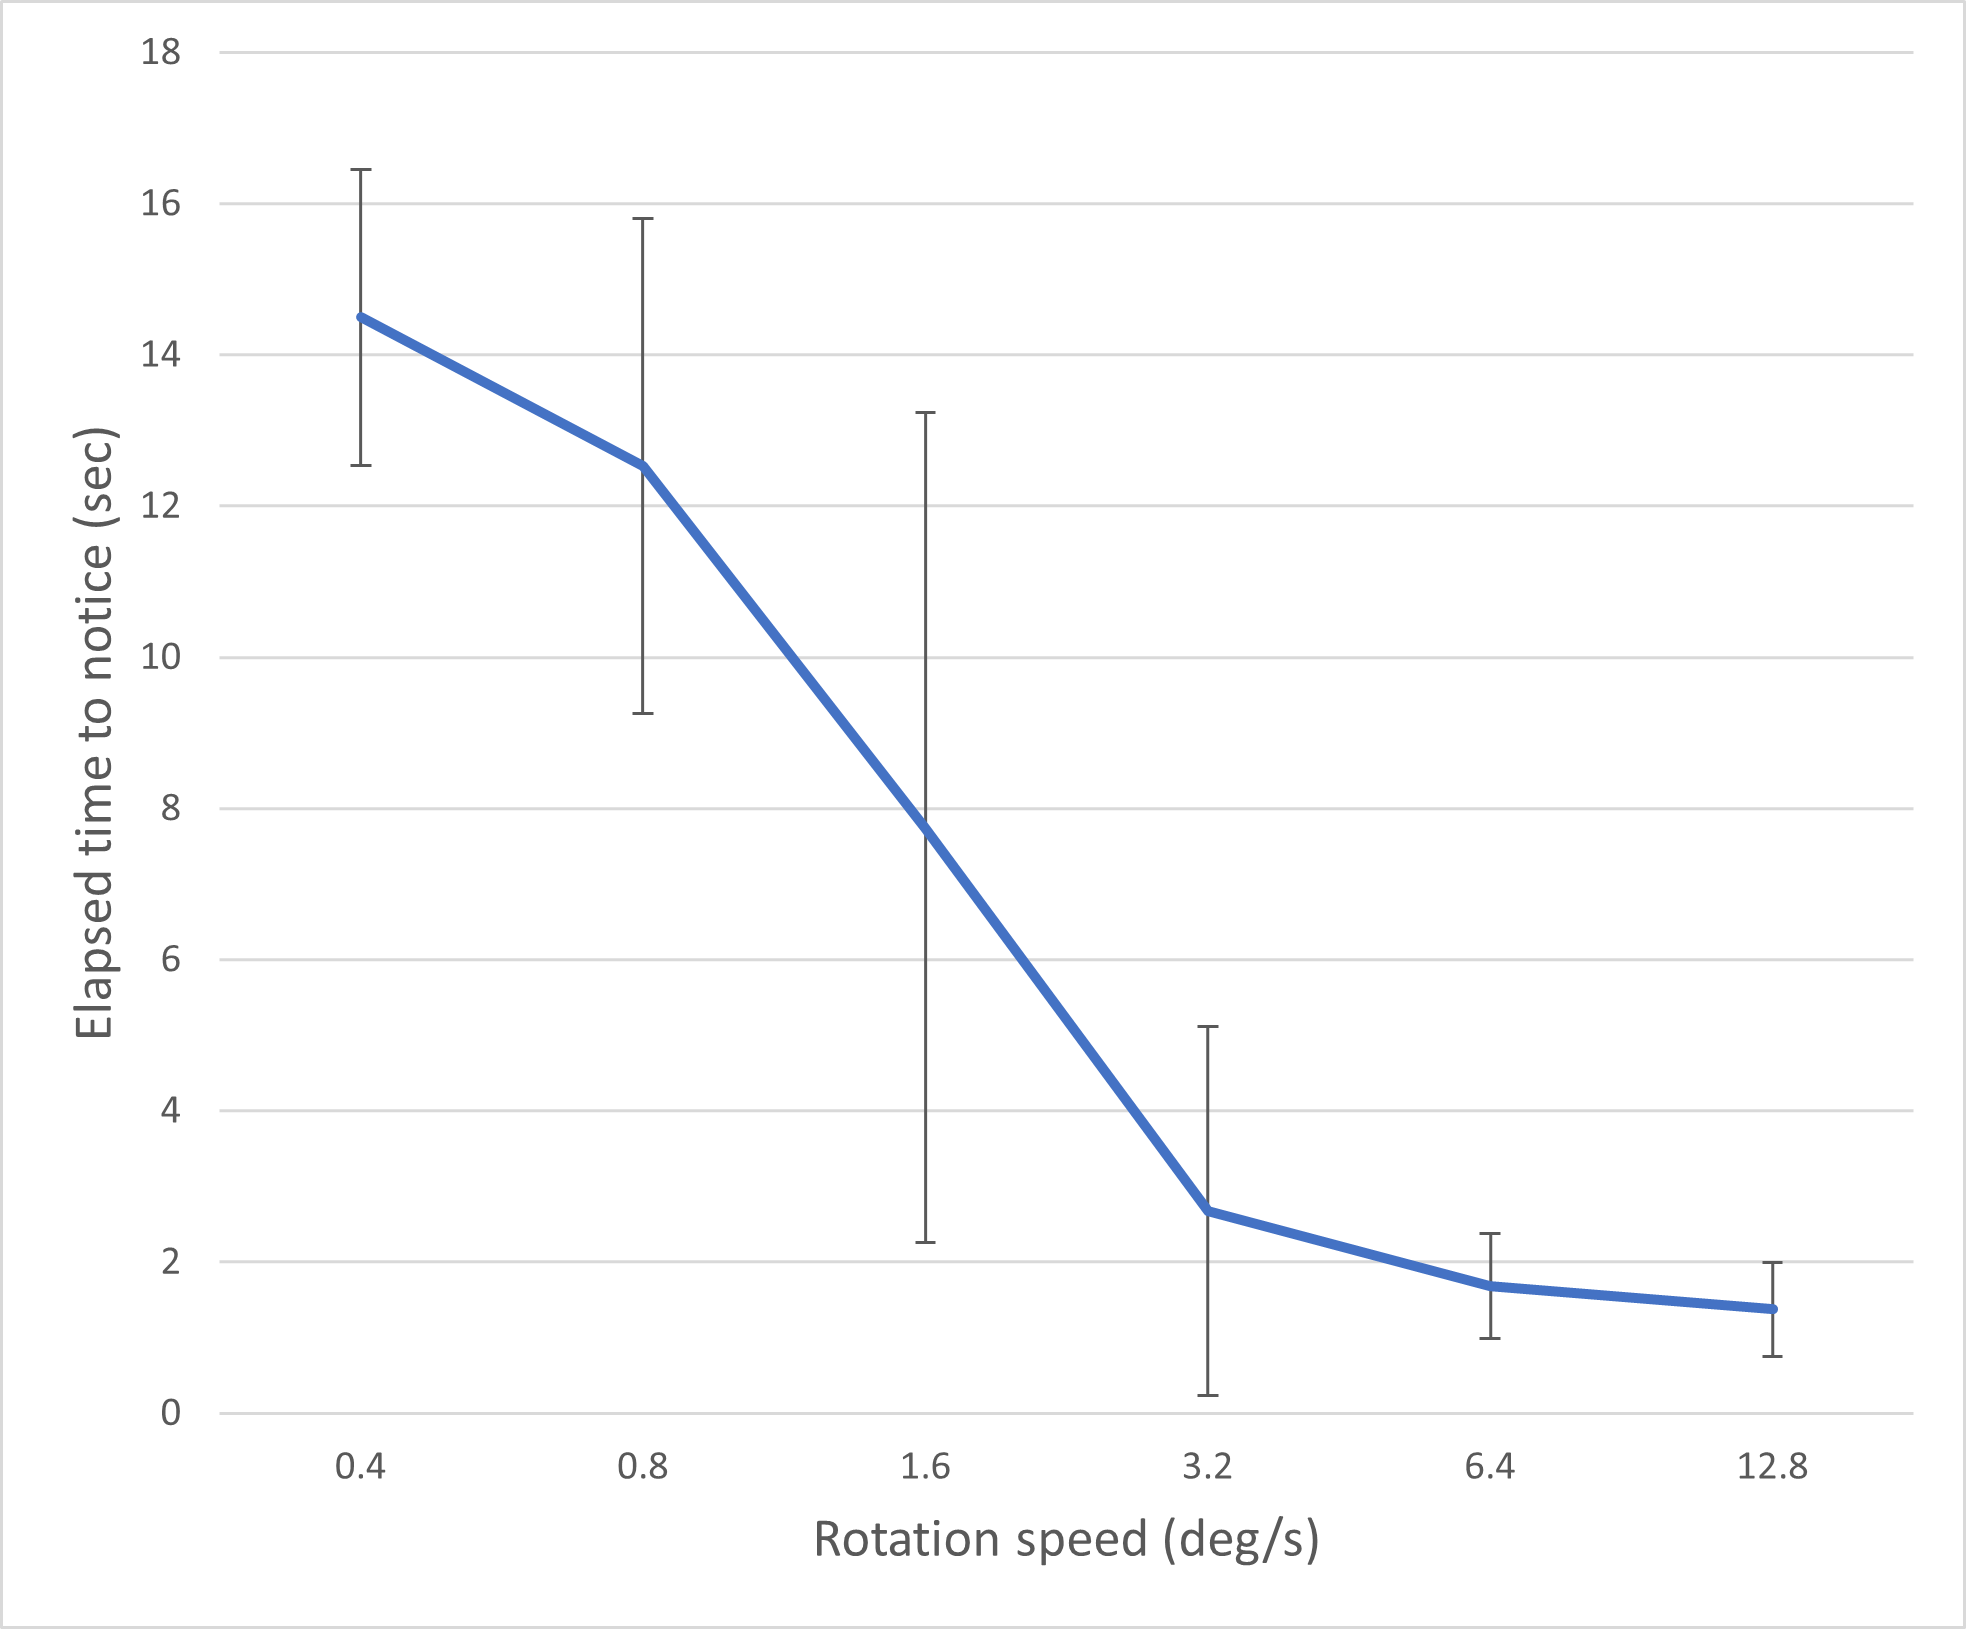
\includegraphics[width=0.8\textwidth]{Pictures/Six constant speeds.png}%imagine location
% 	\caption{Results for stop to constant speed rotation task.}\label{fig:Six constant speeds}%use name for ref.
	
% \end{figure}
% \begin{figure}[H]\centering
% 	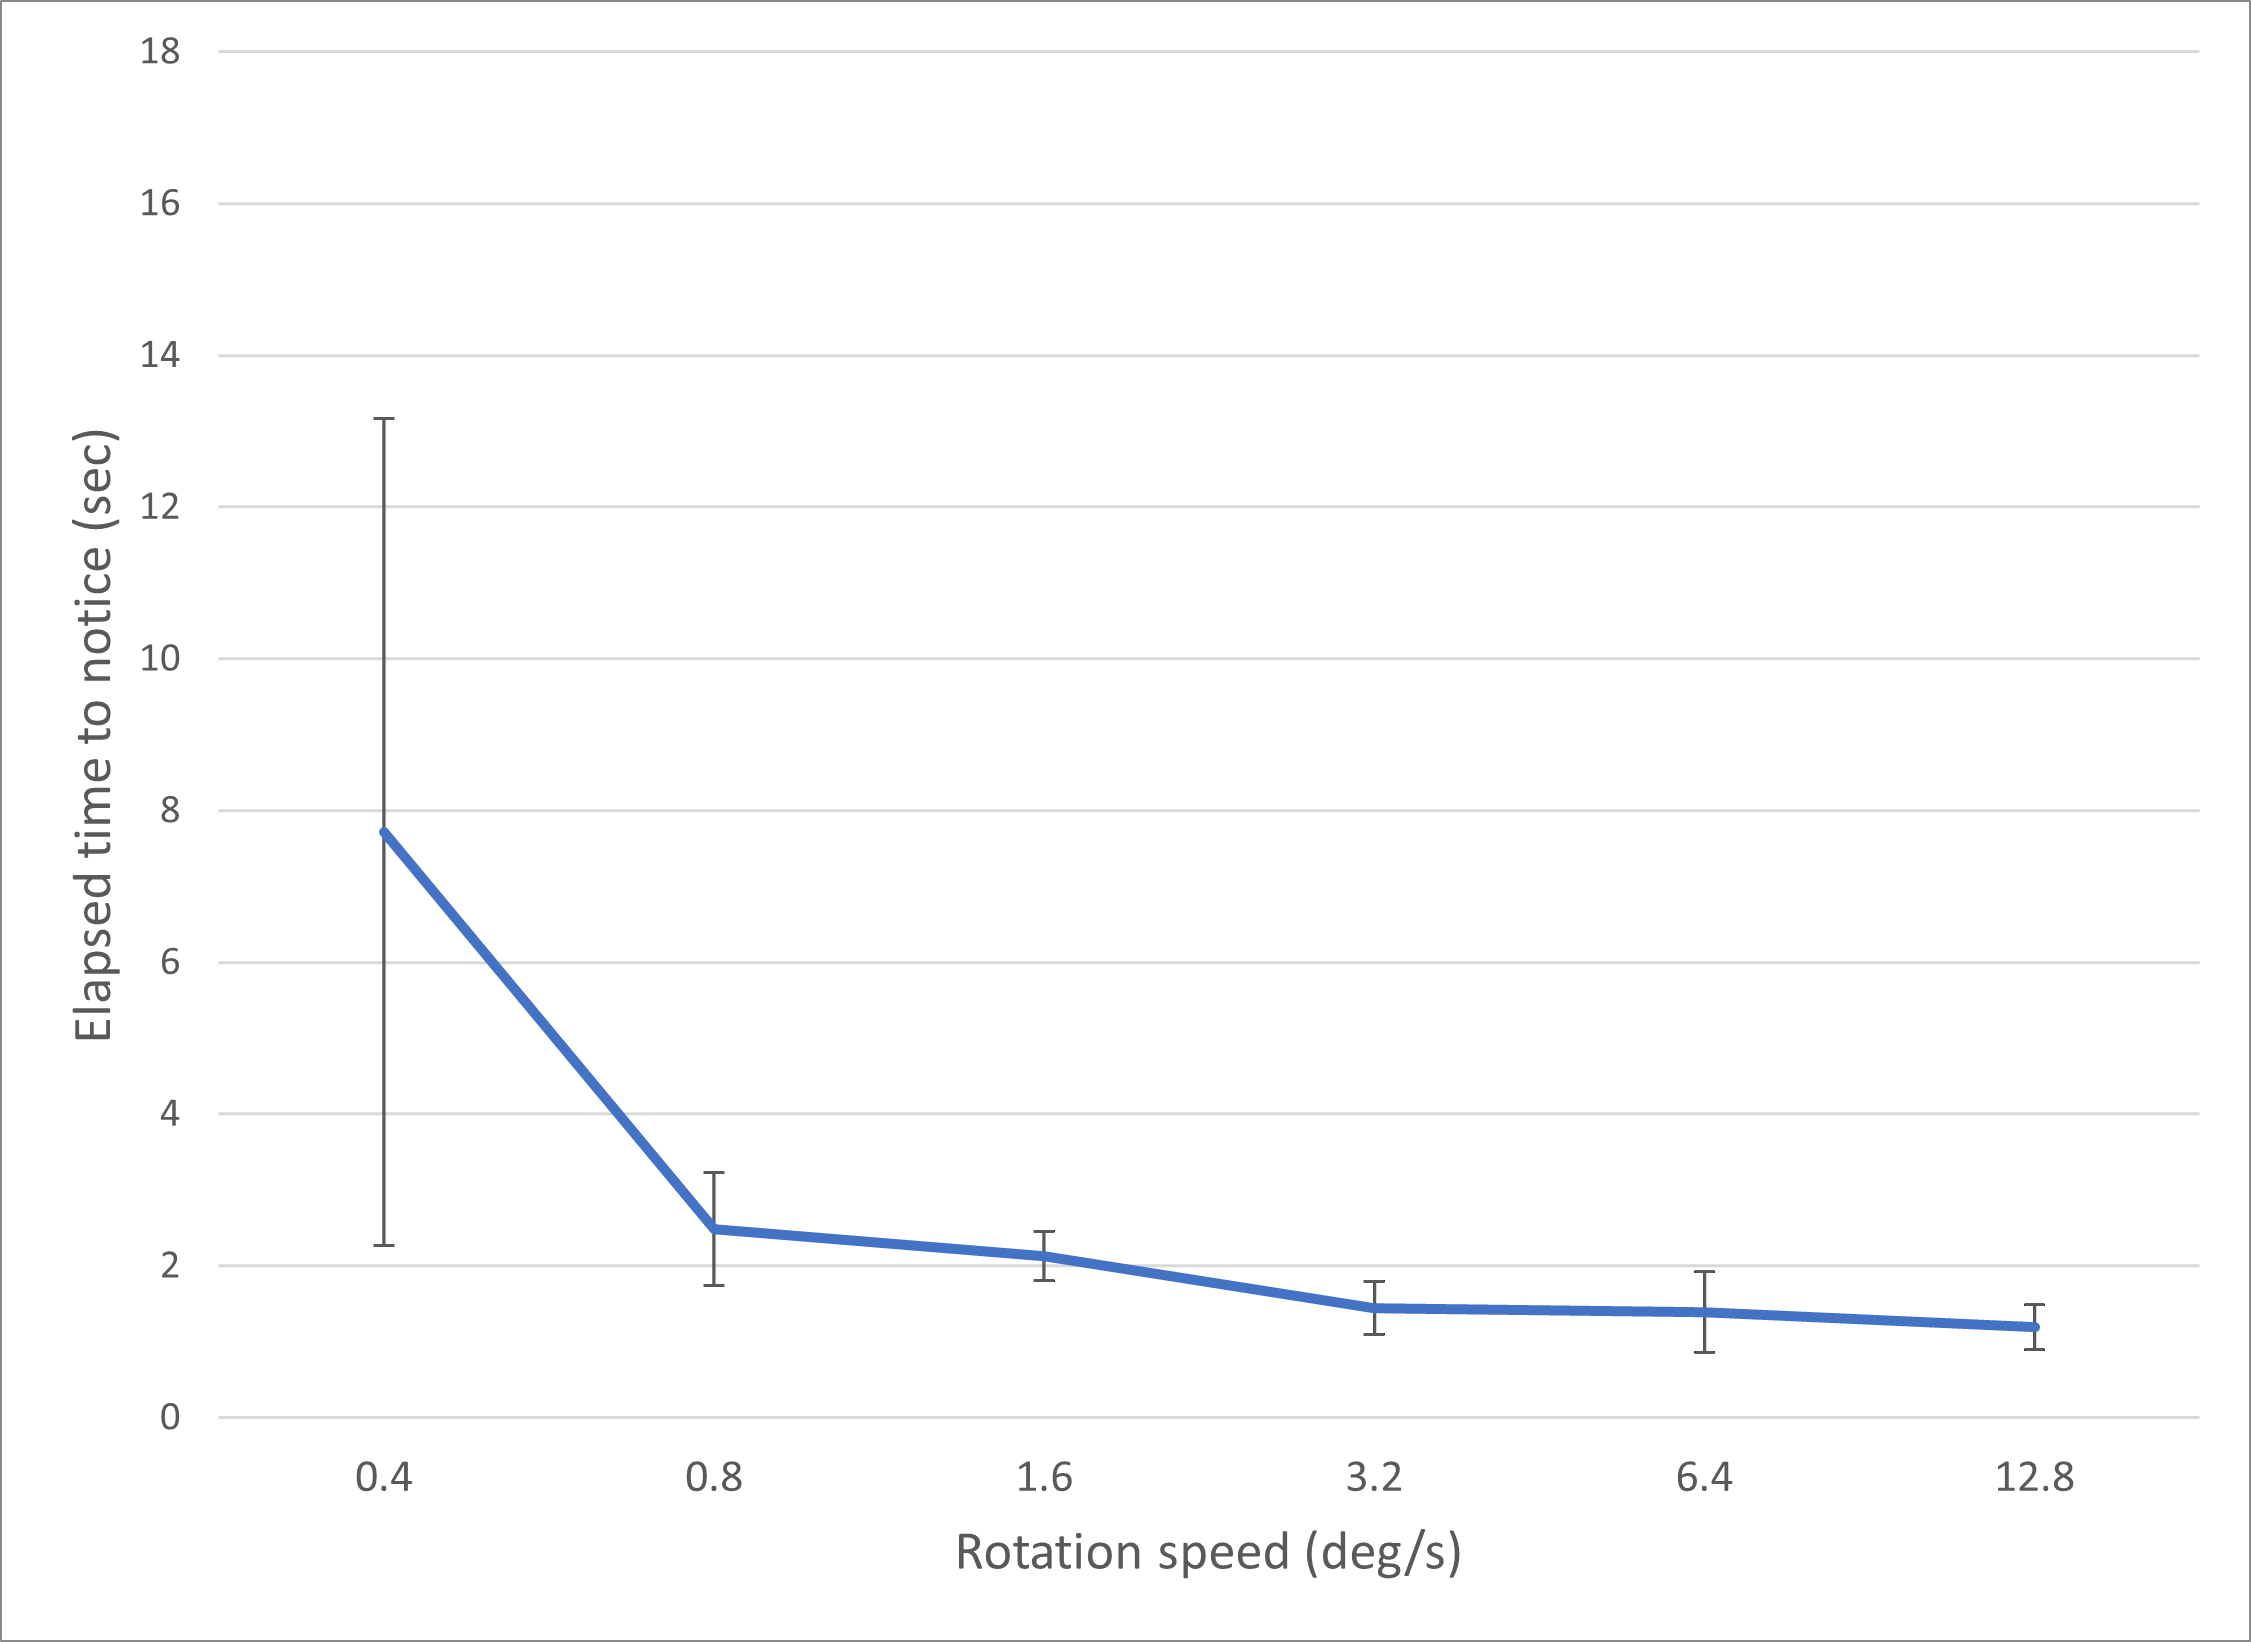
\includegraphics[width=0.8\textwidth]{Pictures/Stop to Six constant speeds.png}%imagine location
% 	\caption{Results for constant speed to stop rotation task.}\label{fig:Stop to Six constant speeds}%use name for ref.
	
% \end{figure}
% \begin{figure}[H]\centering
% 	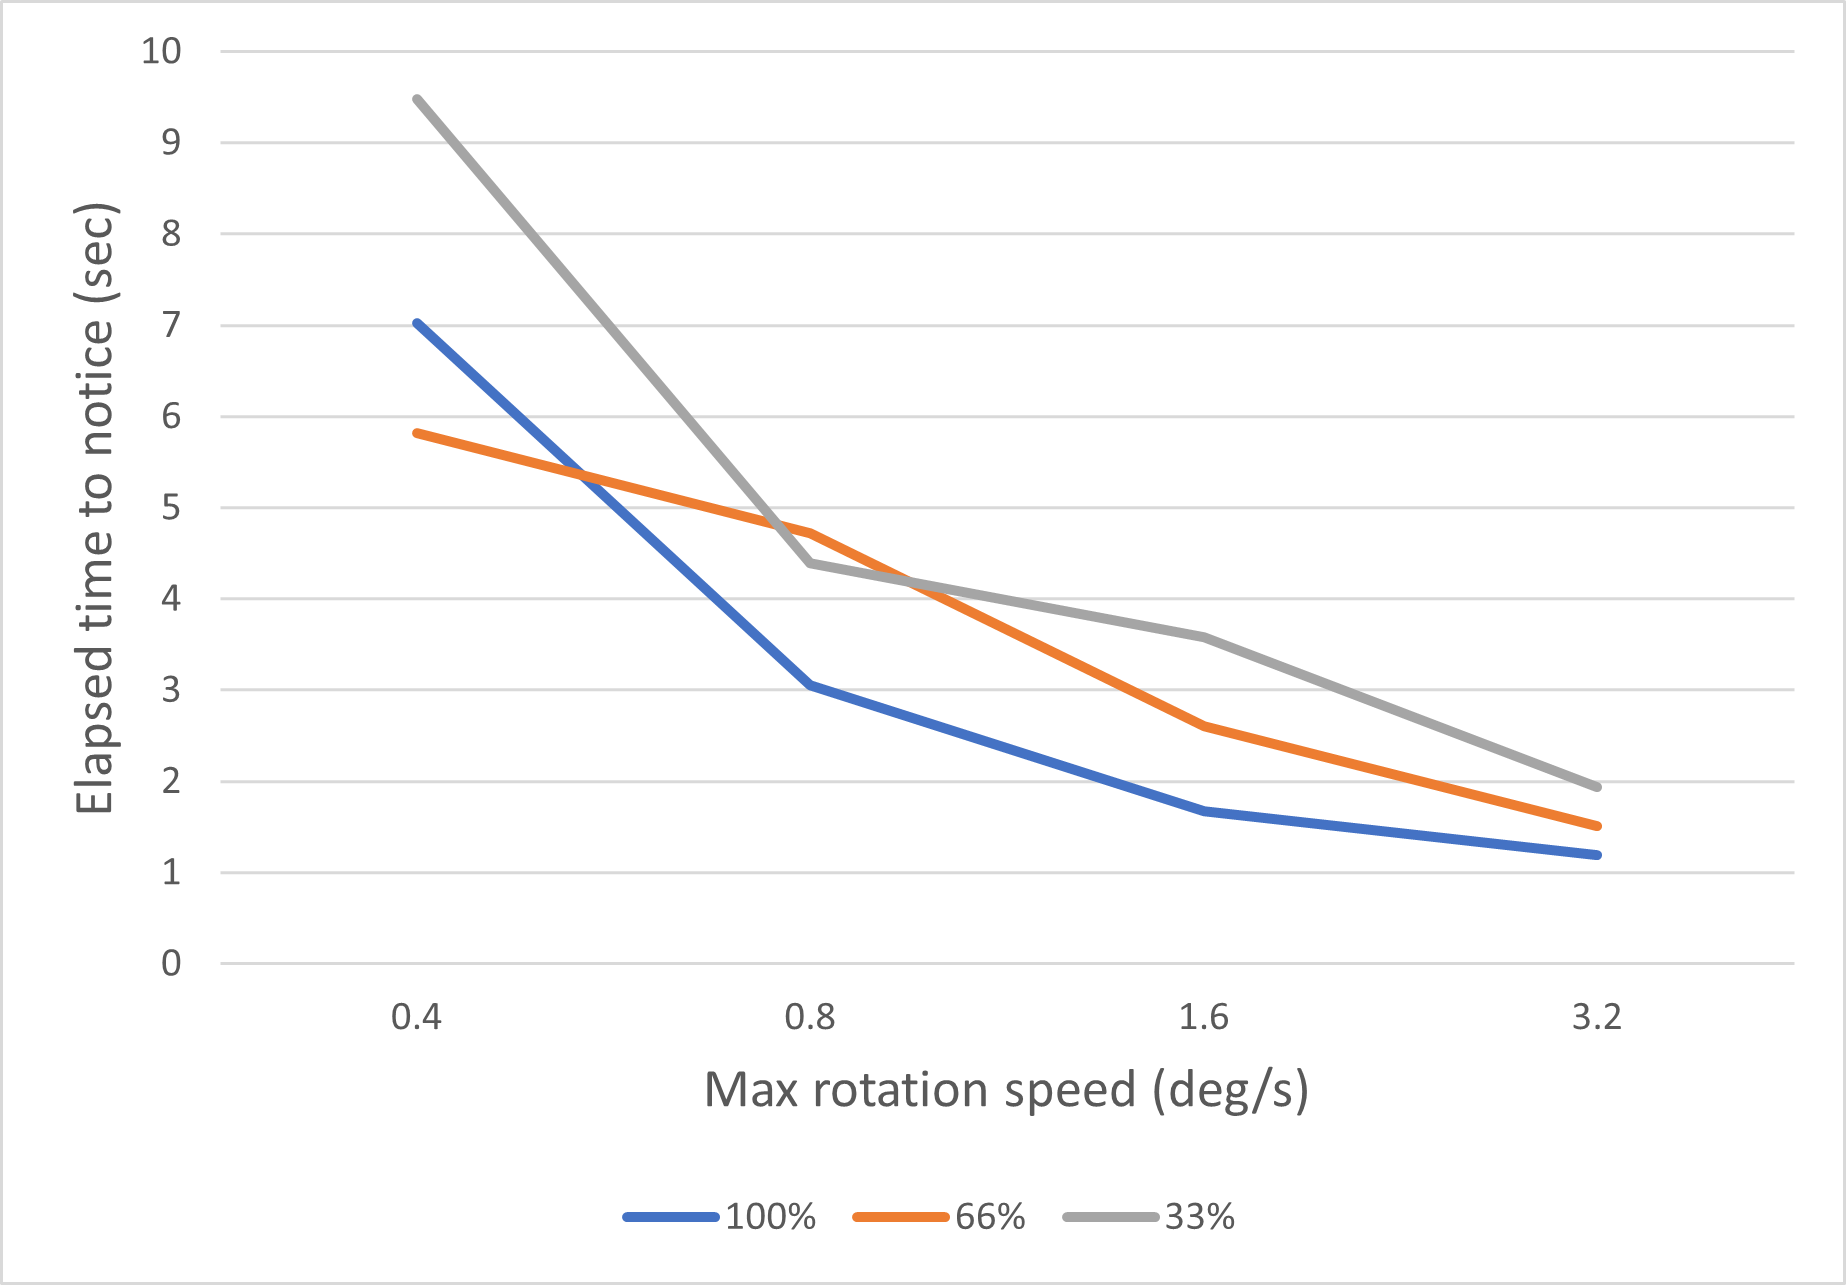
\includegraphics[width=0.8\textwidth]{Pictures/Curvature distance for three decelerations at each constant speed.png}%imagine location
% 	\caption{Results for impact of deceleration of rotation on elapsed time.}\label{fig:Three deceleration of rotation}%use name for ref.
	
% \end{figure}
% \begin{figure}[H]\centering
% 	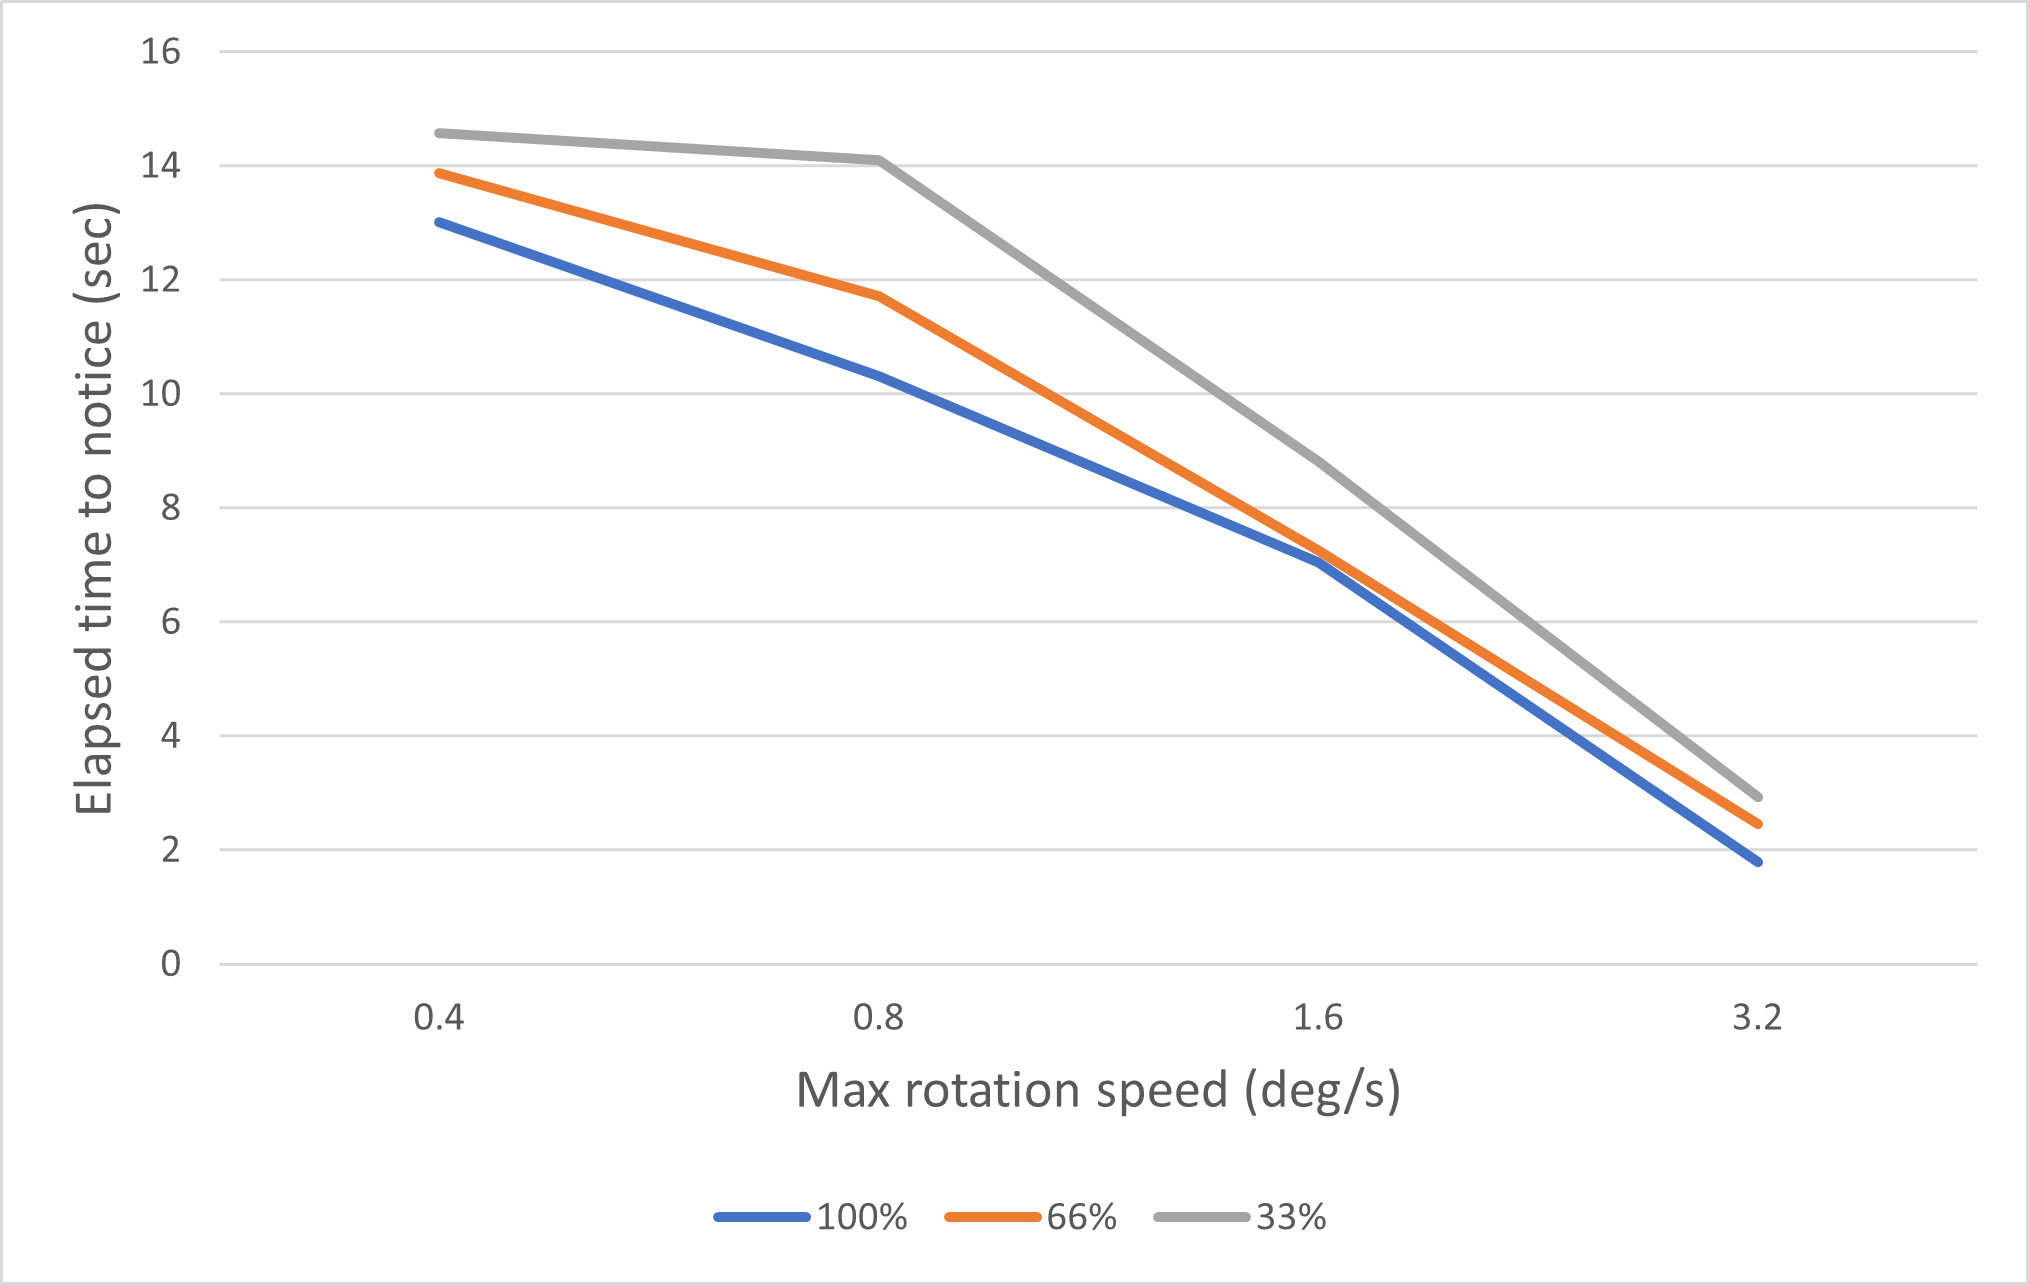
\includegraphics[width=0.8\textwidth]{Pictures/Three acceleration of rotation.png}%imagine location
% 	\caption{Results for impact of acceleration of rotation on elapsed time.}\label{fig:Three acceleration of rotation}%use name for ref.
	
% \end{figure}


% \newpage
% %%%%%%%%%%%%%%%%%%%%%%%%%%%%%%%%%%%%%%%
% %%%%%%%%%%%%%%%%%%%%%%%%%%%%%%%%%%%%%%%
% \section{Curvature distance of humans walking in a rotating virtual environment}
% When multiple users share the same physical space, they might collide. To prevent it, time-dependent synced-rotational gains are applied to the coordinates of their virtual environments so that they would walk in a curved path to away from the collision.

% For properties of the curved path, the purpose of this experiment is to figure out the relation between applied rotational gains and their influence on the curved path.

% \subsection{Curvature distance}
% A curvature distance~\cite{6200791} is the right-angle distance from the straight line to a curved path(Fig.~\ref{fig:CurevDistance}). While a user is walking, the coordinates of his/her HMD will rotate to have him/her walk on a curved path to avoid the collision with other users.
% \begin{figure}[H]\centering
% 	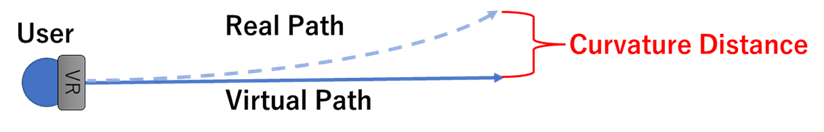
\includegraphics[width=0.9\textwidth]{Pictures/Curvature distance.png}%imagine location
% 	\caption{Curvature distance.}\label{fig:CurevDistance}%use name for ref.
% \end{figure}

% The required curvature distance to swerve the other user coming towards you is the average of half the width of a human shoulder~\cite{9660069}. The half the shoulder width is 23cm.

% \newpage
% \subsection{Experiment tasks}
% In this experiment, two tasks are employed: constant speed task and acceleration task. The constant speed task examines susceptibility of humans' sense of direction to a constant speed of rotation.
% The subject puts on an HMD, then a randomly selected rotation speed (0.4deg/s, 0.8deg/s, 1.6deg/s and 3.2deg/s) is applied to the HMD coordinates while the subject is walking for a specified distance. 

% The acceleration task examines susceptibility of humans' sense of direction to a gradual increase in speed of rotation.
% The initial rotation speed is zero, and a randomly selected rotation speed (0.4deg/s, 0.8deg/s, 1.6deg/s and 3.2deg/s) and a randomly selected acceleration (33\%, 66\% and 100\%) are applied to the HMD coordinates while the subject is walking for a specified distance. Fig.~\ref{fig:Equipment 2} shows a photo taken during the experiment. 
% \begin{figure}[H]\centering
% 	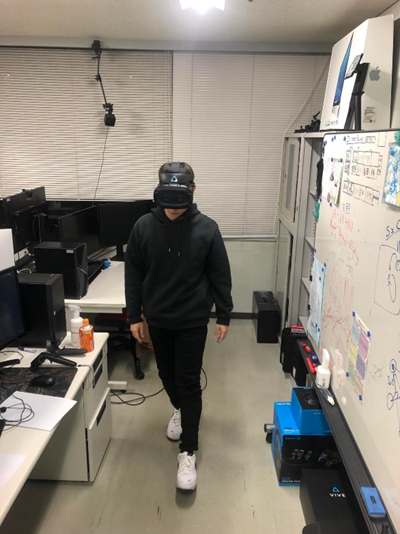
\includegraphics[width=0.4\textwidth]{Pictures/Equipment 2.png}%imagine location
% 	\caption{A scene of the experiment.}\label{fig:Equipment 2}%use name for ref.
% \end{figure}
% \newpage

% \subsection{Procedure} 
% Five subjects with the ages of 25 to 27 years old take part in the experiment.
% \begin{enumerate}
% 	\item Each subject wears an HMD.
% 	\item A rotation speed (0.4deg/s, 0.8deg/s, 1.6deg/s and 3.2deg/s) and a percentage of acceleration (33\%,66\% and 100\%) are randomly selected. 
% 	\item The subject performs the given task (The first task performs the constant speed
% 	task and the second task is the acceleration task).
% 	\item The subject is walking forward for 2 meters at 0.5m/s (the user's walking steps are prescribed by beep sounds)
% 	\item Repeat from step 2 to step 3 at ((4 constant speed x 3 trials) + (4 speed x 3 percentage x 3 trials) = 48 trials)
% \end{enumerate}


% The subjects can take a break every 5minutes to check VR motion sickness symptoms as show in Fig.~\ref{fig:Virtual reality sickness questionnaire_1}.



% \subsection{Data collection}
% For each task, the following data is collected.

% \begin{table}[h!]\centering
% 	\caption{Data collection.}
% 	\label{tab:Data CollectionEx2}%\scriptsize
% 		\scalebox{1.0}{
% 	\begin{tabular}{ |p{4cm}|p{3cm}|p{6cm}|}
% 	\hline
% 		Variable & Unit & Description \\\hline
% 		Curvature distance & centimeter & The right-angle distance of the curvature of the real path relative to the virtual path.\\\hline
% 		Rotation speed & deg/second & Rotation speed of the coordinates of an HMD.\\\hline
% 		Acceleration (for acceleration task) & percentage & Degree of acceleration of the rotation speed.\\\hline
		
% 	\end{tabular}
% 	}
% \end{table} 

% Independent variables are Rotation speed and Acceleration while a dependent one is Curvature distance.




% \newpage

% \subsection{System environment}
% Fig.~\ref{fig:Base State mapping area} shows the top view of a physical space where subjects walk in the experiment. The coordinates of the physical space are defined by two base stations whose positions are known, and the user’s position is tracked and stored in real time.

% By considering the XZ plane, Fig.~\ref{fig:Walking Area in VR} shows the corresponding virtual environment in the experiment where the user moves. The path from the center to the each green box is on the X-axis or Z-axis. The relation between the distance in the virtual environment and the distance in the physical space is one-to-one correspondence.

% \begin{figure}[H]\centering
% 	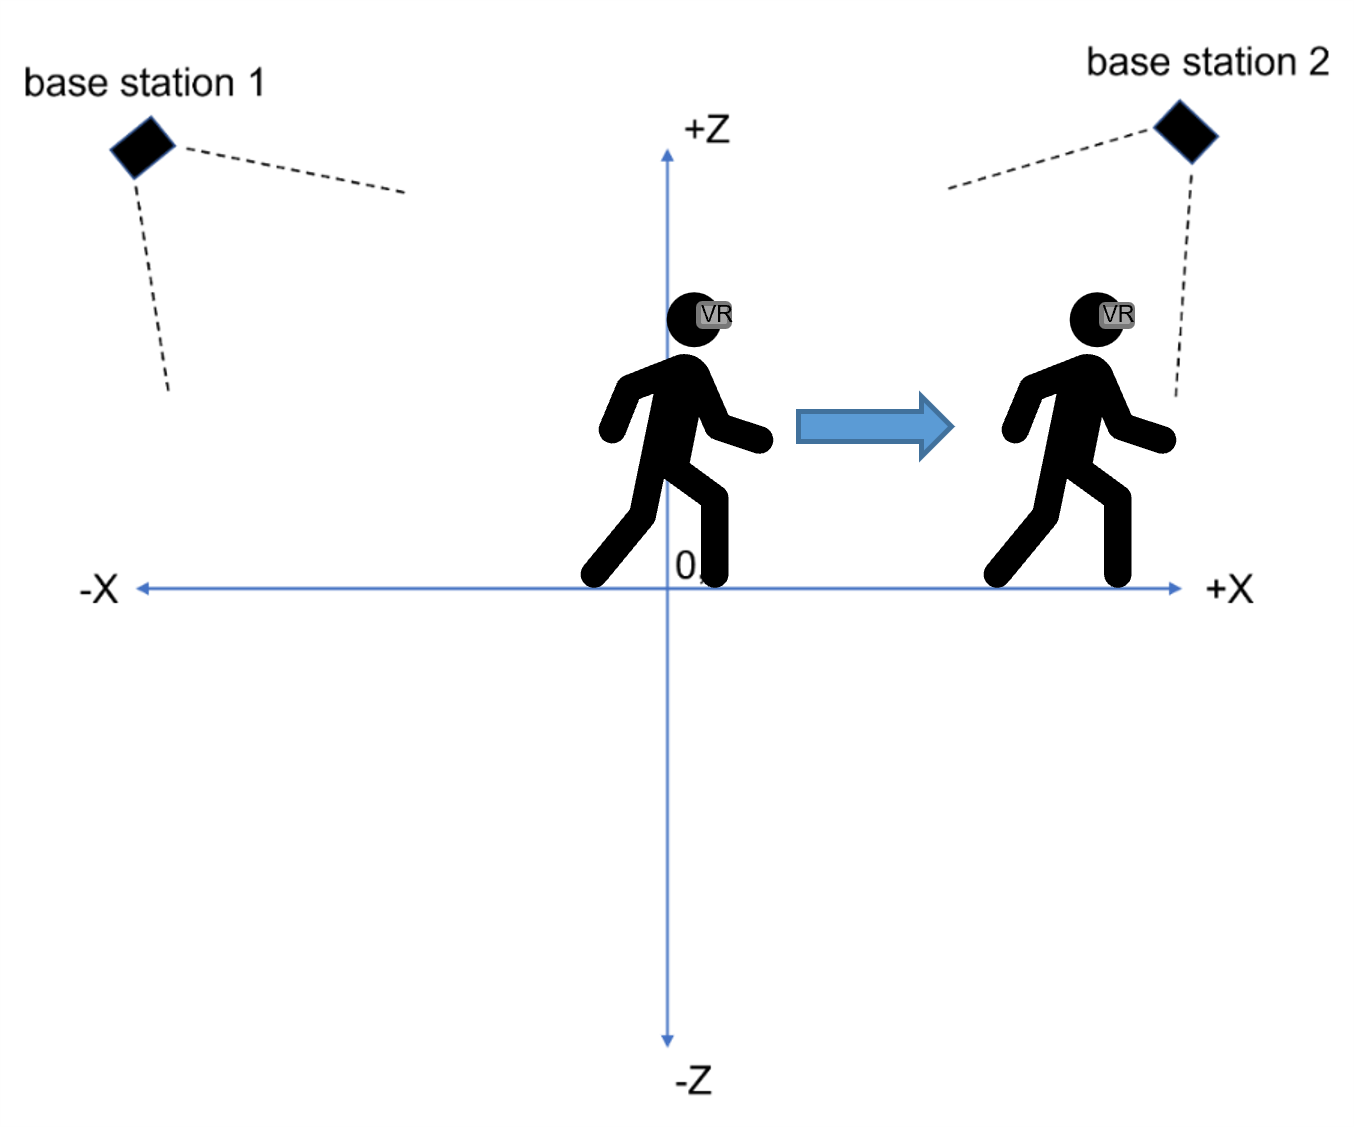
\includegraphics[width=0.7\textwidth]{Pictures/Base State mapping area.png}%imagine location
% 	\caption{Top view of a physical space used in the experiment.}\label{fig:Base State mapping area}%use name for ref.
% \end{figure}
% \begin{figure}[H]\centering
% 	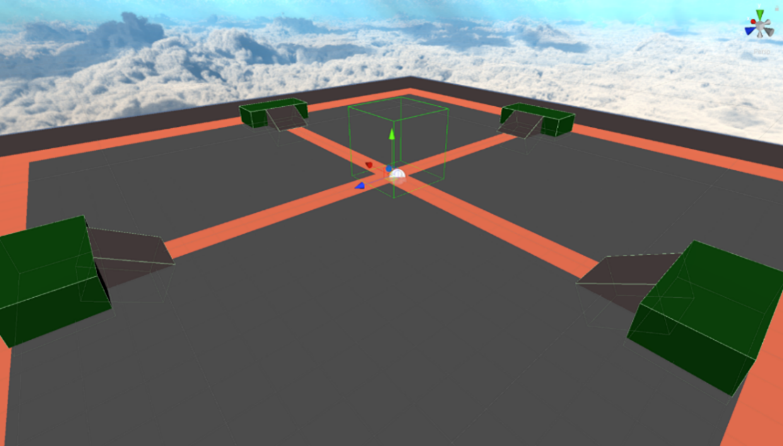
\includegraphics[width=0.7\textwidth]{Pictures/Walking Area in VR.png}%imagine location
% 	\caption{A walking space in a virtual environment.}\label{fig:Walking Area in VR}%use name for ref.
% \end{figure}

% \newpage
% \subsection{Results}
% Fig.~\ref{fig:Curvature distance for four constant speeds} shows a relation between the obtained curvature distance and the given rotation speed. From the figure, the more rotation speed is added the more curvature distance is seen. When the rotation speed is increasing by 1deg/s, the curvature increase around 5.75cm.

% Fig.~\ref{fig:Curvature distance for three accelerations at each constant speed} shows an impact of acceleration in rotation speed on curvature distance. At the degree of acceleration becomes smaller, the curvature distance will decrease a certain amount. When acceleration is increasing by 1\%, the curvature distance will increase by 0.0549cm on average.




% \begin{figure}[H]\centering
% 	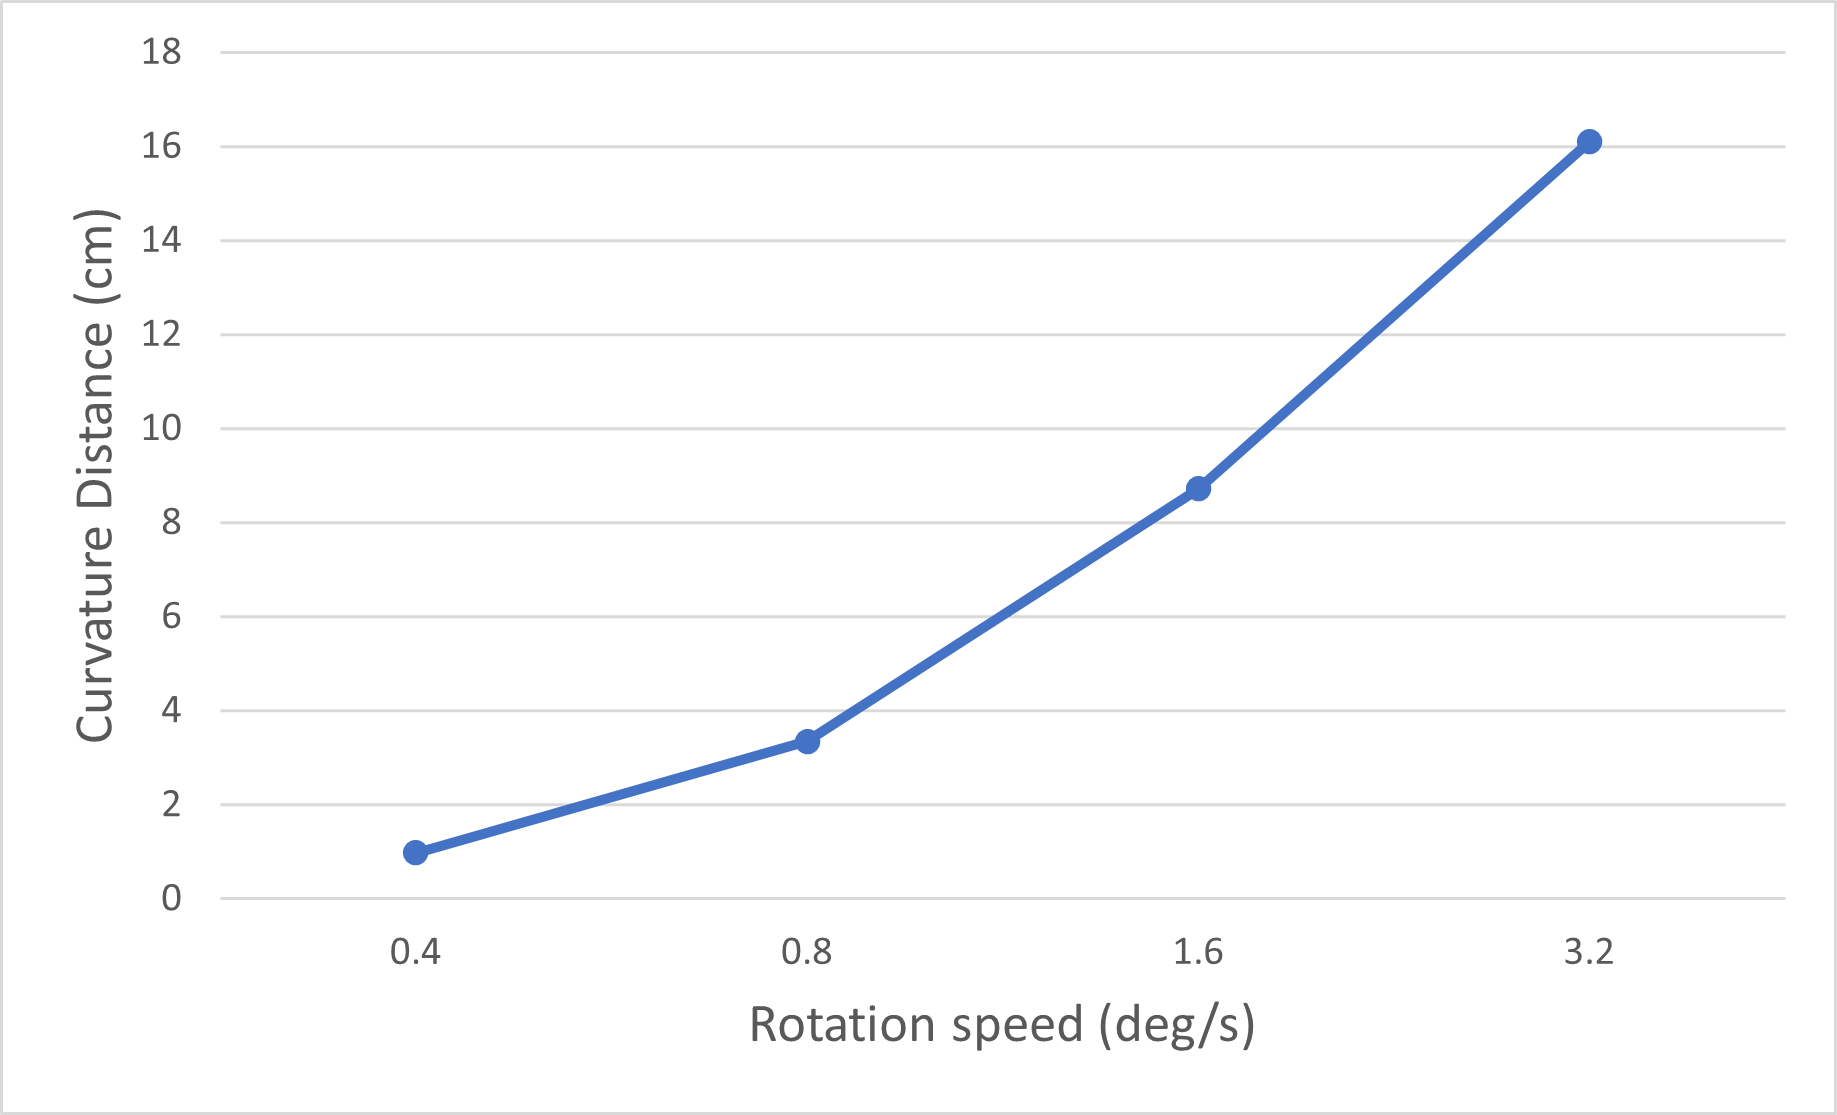
\includegraphics[width=0.8\textwidth]{Pictures/Curvature distance for four constant speeds.png}%imagine location
% 	\caption{Relation between curvature distance and rotation speeds.}\label{fig:Curvature distance for four constant speeds}%use name for ref.
	
% \end{figure}


% \begin{figure}[H]\centering
% 	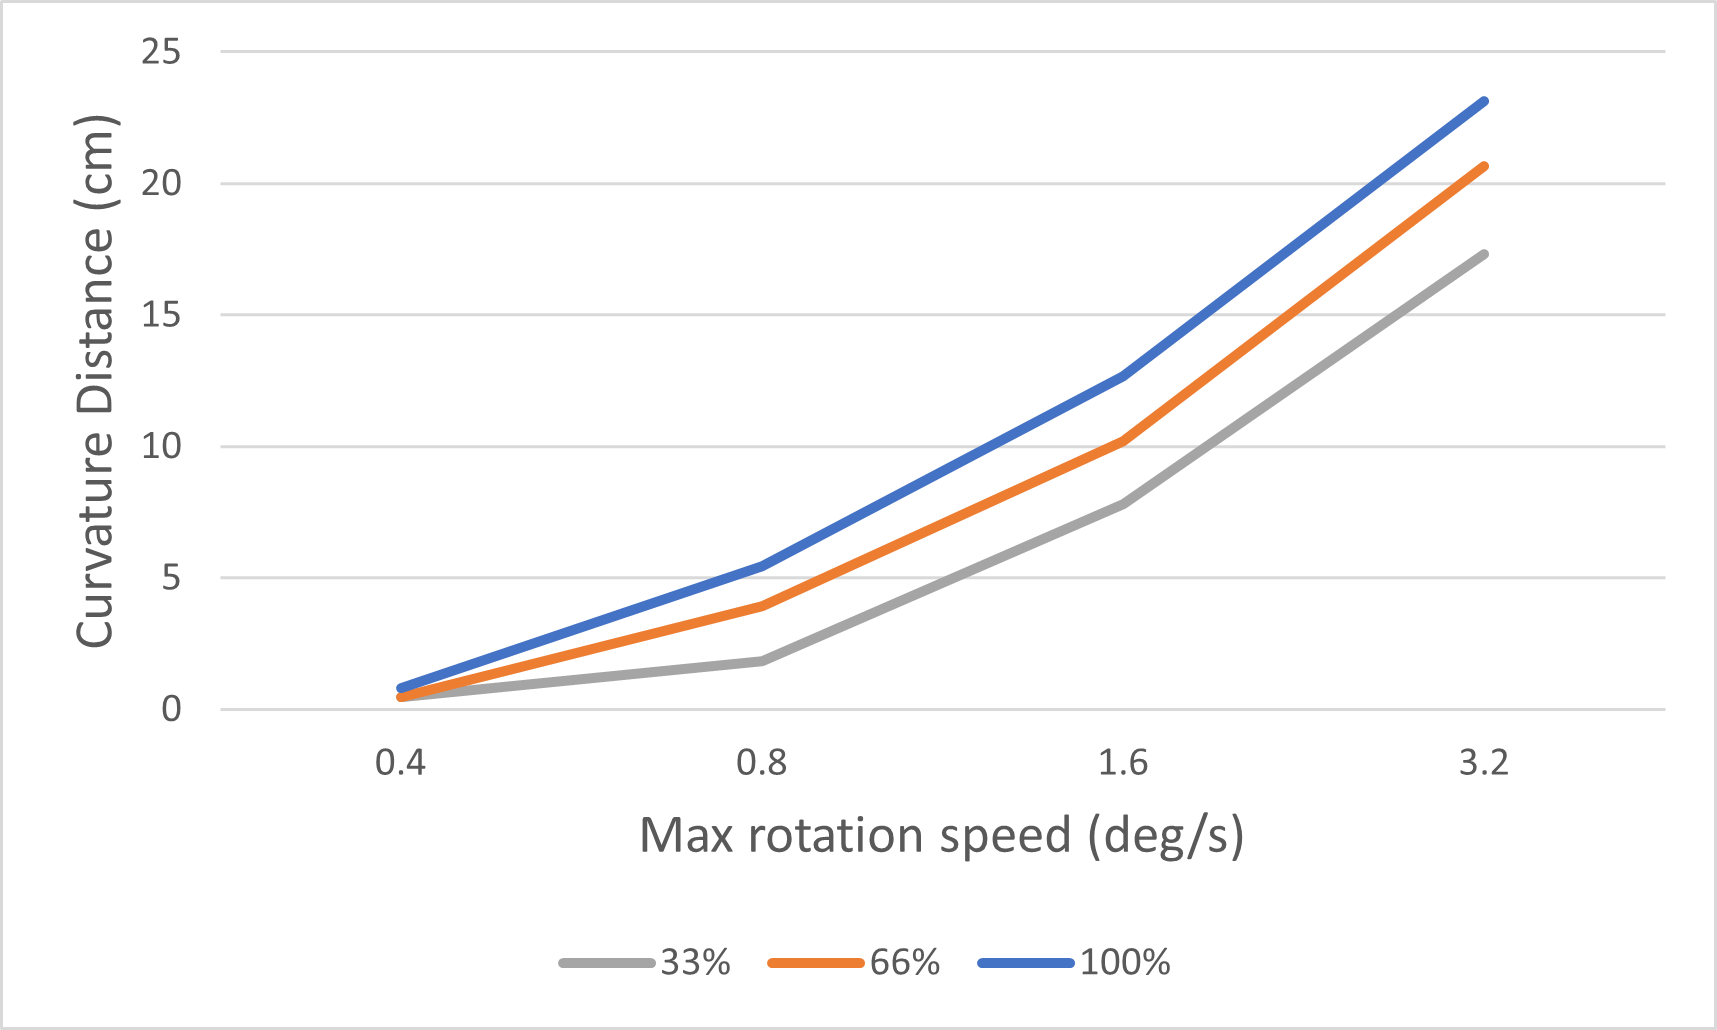
\includegraphics[width=0.8\textwidth]{Pictures/Curvature distance for three accelerations at each constant speed.png}%imagine location
% 	\caption{Relation between curvature distance and acceleration of rotation speeds.}\label{fig:Curvature distance for three accelerations at each constant speed}%use name for ref.
	
% \end{figure}


% \begin{figure}[H]\centering
% 	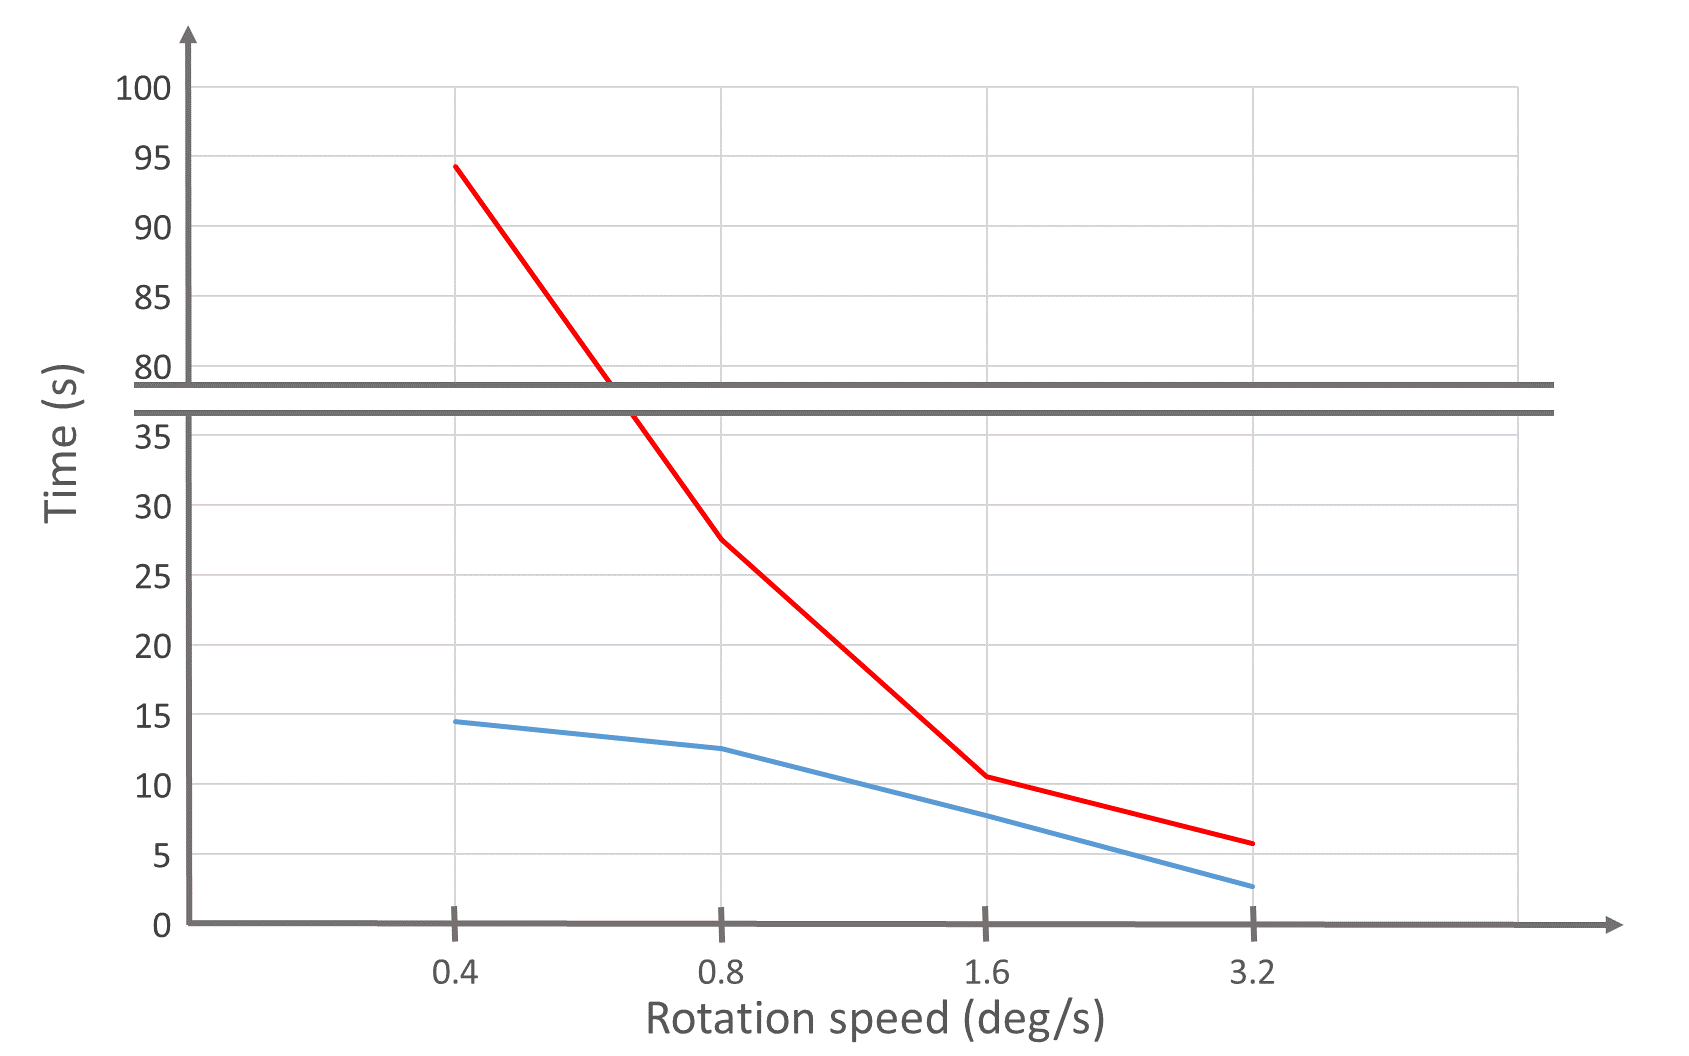
\includegraphics[width=0.9\textwidth]{Pictures/edit.png}%imagine location
% 	\caption{Result between sensitivity of rotational awareness of humans (blue line) and curvature distance of humans walking (red line) in VR.}\label{fig:Exp2_Conclude}%use name for ref.
	
% \end{figure}

% Fig.~\ref{fig:Exp2_Conclude} shows a condition to perform the proposed method where a user is not aware of the rotation, and he/she swerves by half the shoulder width. The horizontal axis shows the rotation speed of the virtual environment in degrees per second and the horizontal one does the elapsed time in second. The blue line represents the elapsed time on average users spend until they become aware of rotation for each rotation speed. The red one represents the elapsed time on average users spend until they make 23cm of the curvature distance at the walking speed of 0.5m/s for each rotation speed. The red line is calculated from the values from Fig.~\ref{fig:Curvature distance for four constant speeds}. From the two lines, users can not avoid a collision without awareness of rotation because the time it takes to be aware of rotation is shorter than the time it takes to make the curvature distance of 23cm.

% \newpage
% \begin{figure}[H]\centering
% 	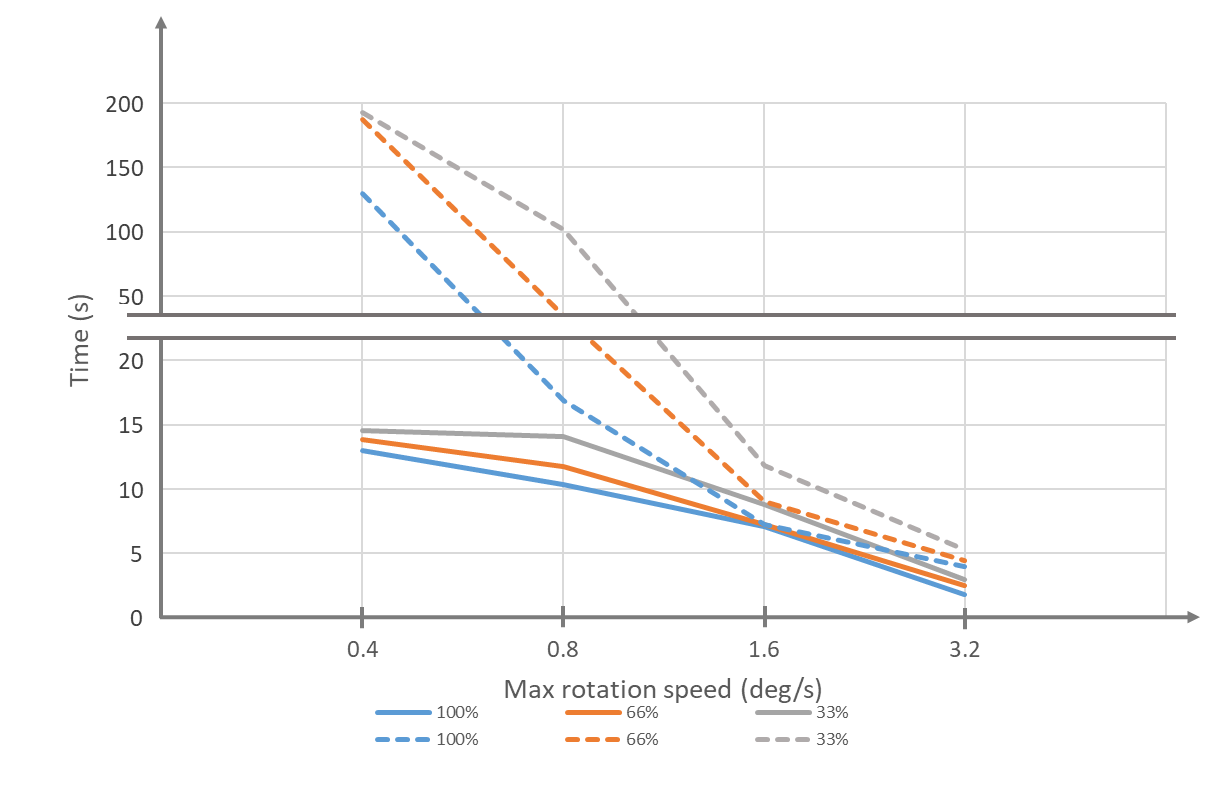
\includegraphics[width=1.0\textwidth]{Pictures/CurvatureDistanceandTimes.png}%imagine location
% 	\caption{Result between Sensitivity of Rotational Awareness of Humans (solid line) and Curvature Distance of Humans Walking (dash line) in VR.}\label{fig:Exp2_ConcludeOfacceration}%use name for ref.
% \end{figure}

% Fig.~\ref{fig:Exp2_ConcludeOfacceration} shows a condition to perform the proposed method where a user swerves by half the shoulder width while being unaware of it for each acceleration. The horizontal axis is the max rotation speed of the virtual environment, to which the rotation speed increases from zero. The horizontal axis is the elapsed time in second. For each max rotation speed, the solid line shows the average amount of time it takes for users to become aware of rotation with acceleration. The dashed line shows how long it takes for users to cover 23cm of the curvature distance at a speed of 0.5m/s for each max rotation speed. The solid line and the dashed line are calculated from Fig.~\ref{fig:Three acceleration of rotation} and Fig.~\ref{fig:Curvature distance for three accelerations at each constant speed}. The gray line presents an acceleration of 33\%, the orange line presents an acceleration of 66\%, and the blue line gives an acceleration of 100\%. From these results, the proposed method is capable of having users swerve by half the shoulder 23cm without awareness of rotation at the max rotation speed of 1.6 deg/s and acceleration of 100\% at the duration of about 8 seconds.



\chapter{Experiment} % Main chapter title

\label{Chapter4} % Change X to a consecutive number; for referencing this chapter elsewhere, use \ref{ChapterX}



%----------------------------------------------------------------------------------------
%	SECTION 1
%----------------------------------------------------------------------------------------



To evaluate the effectiveness and practicality of the developed wearable haptic glove, I conducted two structured experiments focusing on both perceptual discrimination and subjective realism of vibrotactile feedback. 
In Experiment 1, I assessed participants' ability to distinguish between three distinct vibration cycle rates delivered through the glove. 
In Experiment 2, I investigated the relationship between the vibration cycle rates and the perceived realism of various virtual textures. 
Together, these experiments provided both quantitative performance data and qualitative user feedback, offering a comprehensive evaluation of the glove’s performance in enhancing virtual texture perception and supporting natural hand interactions in virtual reality applications.

\section{Equipment and Specifications}
The experimental setup included a desktop host machine with an Intel® Core™ i7-13700 processor, an NVIDIA® GeForce RTX™ 3050 graphics card, and 16 GB of system memory. This configuration provided adequate computational power for rendering real-time virtual environments and processing haptic feedback with low latency. The virtual environment was developed using Unity 2022.3.23f1 (LTS), which offered a stable platform for implementing custom interactions and integrating external hardware devices.

The wearable haptic glove, developed in this study, was connected to the host system. The glove’s onboard microcontroller handled real-time sensor data acquisition and vibration control, while Unity managed virtual object interactions and feedback synchronization. This combination of hardware and software provided a responsive and immersive environment for evaluating virtual texture perception and gesture-based control in virtual reality, shown in Fig.~\ref{fig:experiment}.

\begin{figure}[H]\centering
	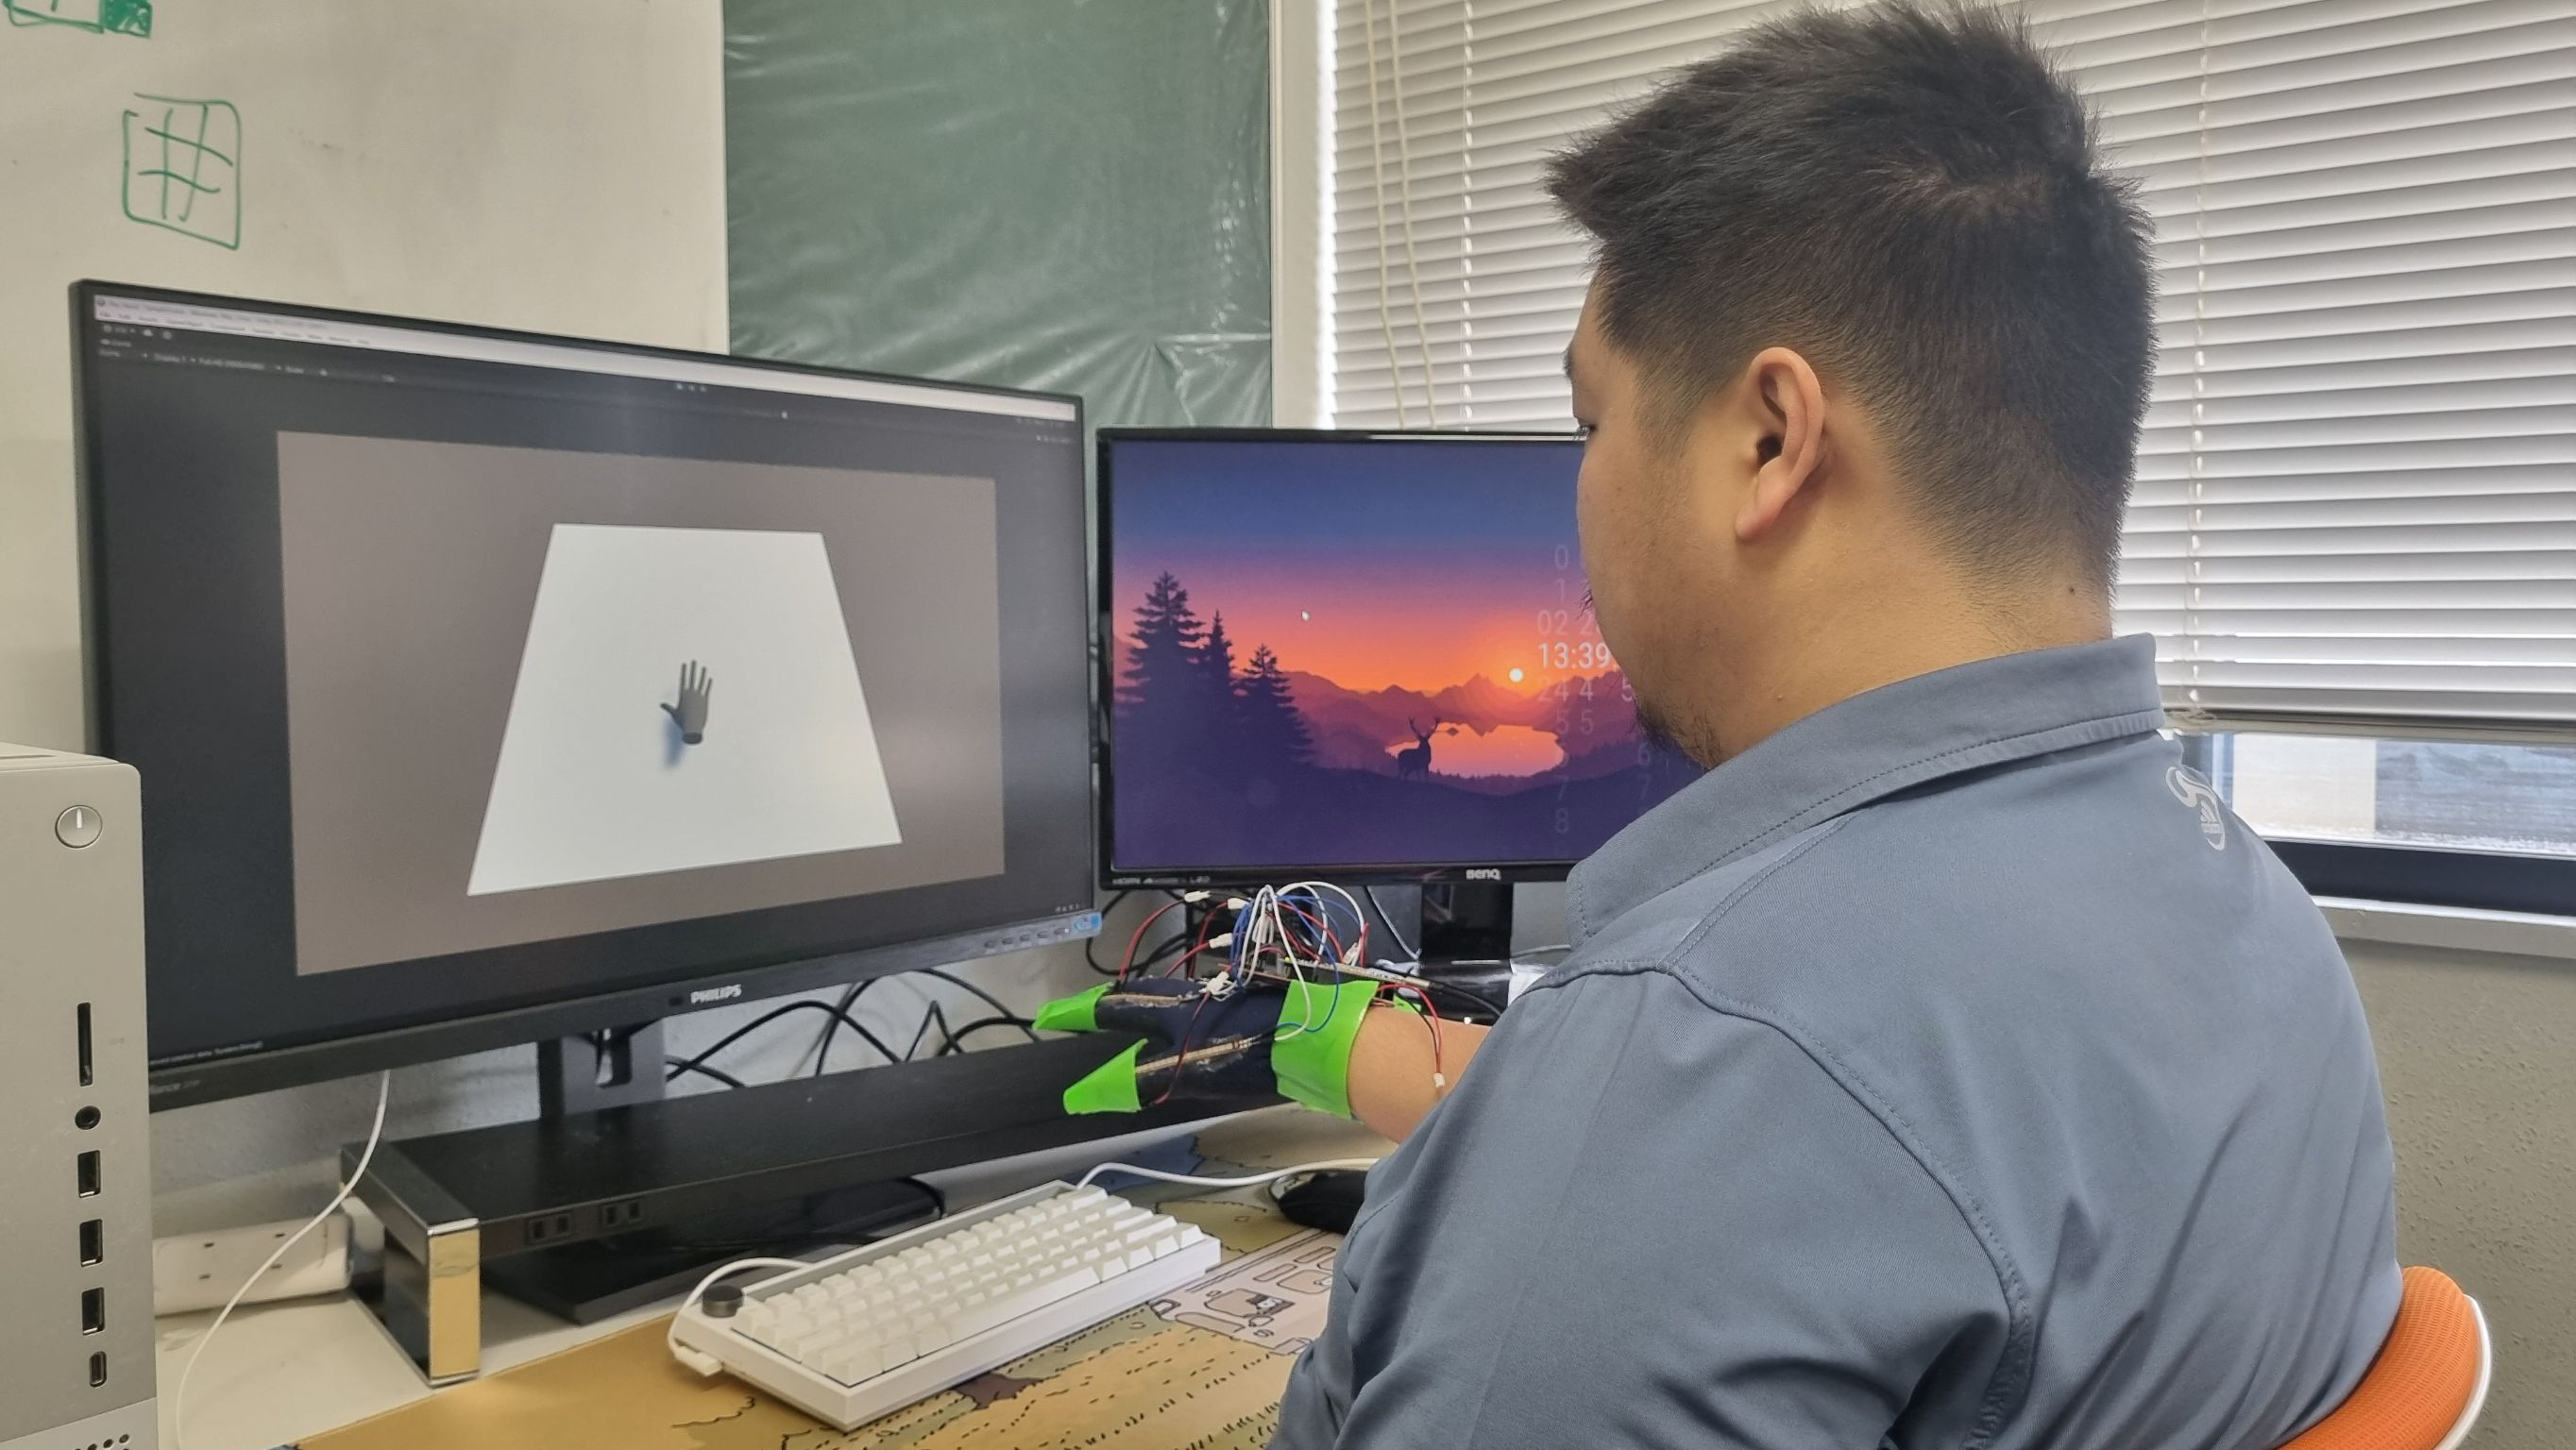
\includegraphics[width=0.9\textwidth]{Pictures/experiment.png}%imagine location
	\caption{Overall experimental setup demonstrating participant interaction using the wearable haptic glove}\label{fig:experiment}%use name for ref.
	
\end{figure}
%%%%%%%%

\newpage
\section{Haptic Feedback Method}

In this experiment, the haptic feedback method utilizes PWM (Fig.~\ref{fig:pwm_2}) to create vibrotactile sensations that simulate variations in surface texture within virtual environments. The goal of this feedback mechanism is to provide tactile cues that represent different levels of surface roughness and bumpiness, thereby increasing the realism of virtual interactions. This section outlines the signal generation process, cycle rate configuration, vibration pattern design, and how these elements are integrated into the overall virtual reality system.

\begin{figure}[H]\centering
	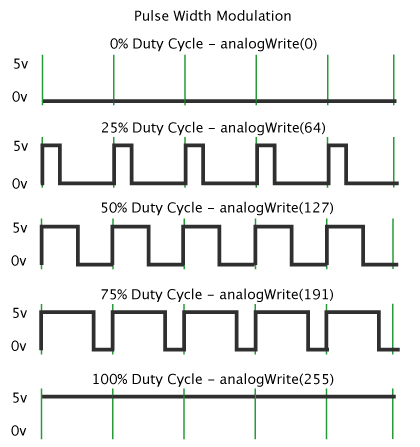
\includegraphics[width=0.7\textwidth]{Pictures/PWM_2.png}%imagine location
	\caption{PWM behavior\cite{pwm_doc}}\label{fig:pwm_2}%use name for ref.
	
\end{figure}

\subsubsection{PWM-Based Vibration Control}
PWM is a method of signal modulation in which a digital output rapidly switches between on and off states. The duration for which the signal is in the ``on" state during each cycle, known as the duty cycle, determines the effective power delivered to the actuator. In this system, the ESP32 microcontroller generates PWM signals through its dedicated hardware PWM channels. This ensures high-frequency, low-latency signal control, making it suitable for real-time virtual reality applications.

\newpage
\subsubsection{Duty Cycle Settings}
In Fig.~\ref{fig:pwm_3}, the duty cycle was set to fixed values of 0.2, 0.5, and 1.0 to ensure a consistent vibration intensity during each active phase. Preliminary testing revealed that maintaining a constant duty cycle allowed the vibration motor to achieve a noticeable amplitude without causing discomfort. This method helps avoid the variability in perceived intensity that can arise from fluctuating duty cycles, enabling the study to concentrate solely on the effects of vibration rhythm and cycle rate.

\begin{figure}[H]\centering
	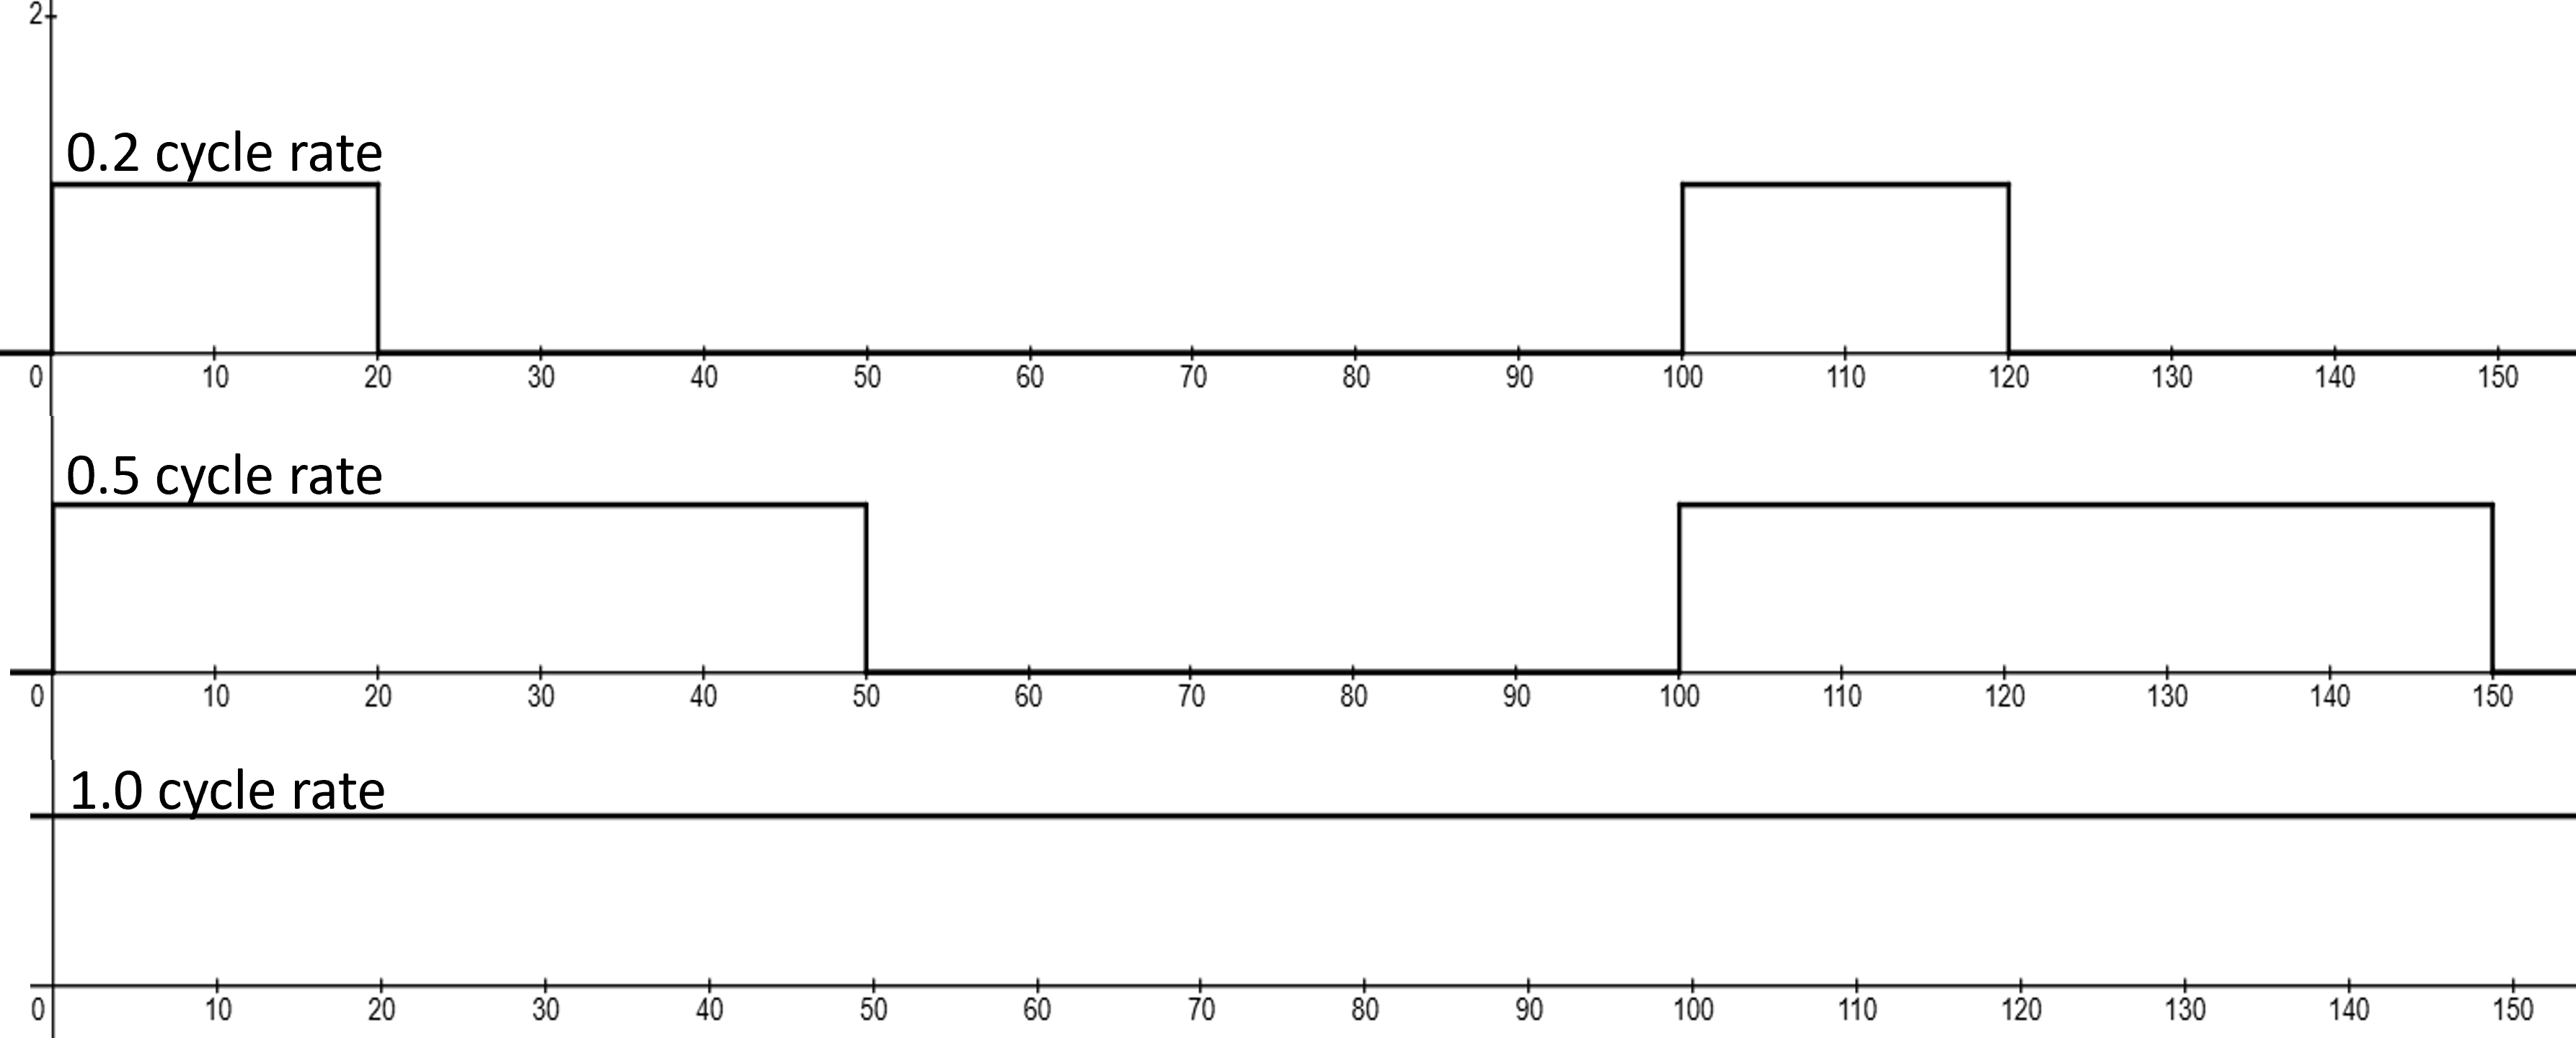
\includegraphics[width=1\textwidth]{Pictures/PWM_3.png}%imagine location
	\caption{PWM with different cycle rates}\label{fig:pwm_3}%use name for ref.
	
\end{figure}

To simulate differences in texture, the cycle rate—defined as the interval at which the motor alternates between active (vibrating) and inactive (paused) states—was adjusted while maintaining a constant PWM duty cycle. Three distinct cycle rates were designed to represent various virtual textures:

\begin{itemize}
  \item \textbf{Low cycle rate (0.2)}: This is characterized by longer on-off intervals, creating a rough, bumpy tactile sensation.
  \item \textbf{Medium cycle rate (0.5)}: This feature moderates pulse intervals, producing a balanced sensation suitable for medium-textured virtual surfaces.
  \item \textbf{High cycle rate (1.0)}: This involves rapid successive pulses with minimal pauses, resulting in a smooth and continuous tactile impression.
\end{itemize}

This method offers a straightforward yet effective way to represent textural properties by focusing on temporal vibration patterns rather than changing vibration amplitude.
%%%%%%%%

\newpage
\section{Experiment}

\subsection{Experiment 1: Distinguishing Haptic Feedback}
I recruited a total of six participants, all right-handed and aged between 24 and 27 years, for the first experiment. None of the participants had prior experience with the specific haptic device and reported no known sensory or motor impairments. The primary aim of this experiment was to conduct a blind classification test to evaluate their ability to reliably distinguish between three predefined vibration cycle rates: 0.2, 0.5, and 1.0 cycles per second. These cycle rates were chosen to represent three distinct levels of vibration rhythm, intended to simulate variations in virtual surface textures.

Before the formal testing session, all participants went through a familiarization phase where they experienced each of the three cycle rates individually. During this phase, each cycle rate was presented multiple times in a labeled, non-randomized order. This allowed participants to establish a clear tactile reference for the “low,” “medium,” and “high” vibration patterns. Participants were encouraged to ask questions and could repeat the familiarization process as needed to ensure they fully understood each vibration profile before moving on to the blind testing phase. This preparation aimed to minimize learning effects during the main experiment and ensure that the evaluation focused solely on the participants' ability to discriminate tactile sensations.

\textbf{Procedure:} Participants wore and calibrated the glove through repeated hand opening and closing gestures, ensuring accurate hand tracking. Subsequently, participants interacted with a plain white 3D plane in the virtual environment (Fig.~\ref{fig:experiment1_setup}), triggering randomly generated vibrations corresponding to one of the three cycle rates. Participants verbally identified the perceived cycle rate after each interaction. Each participant completed 15 randomized trials, assessing their discrimination accuracy.

\begin{figure}[H]\centering
	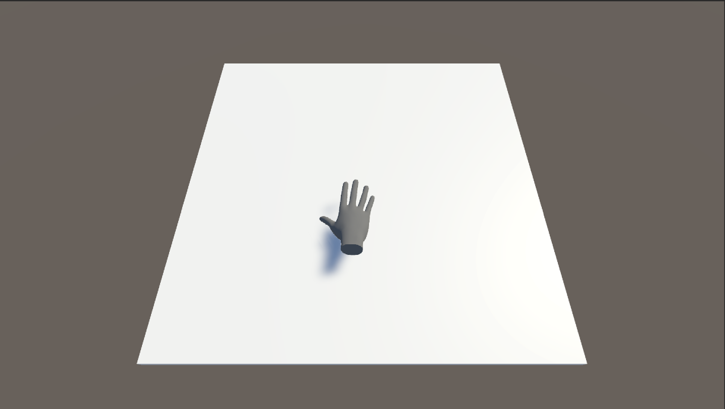
\includegraphics[width=1\textwidth]{Pictures/ex1.png}%imagine location
	\caption{Experimental setup for Experiment~1: participants interacting with a plain white virtual plane to distinguish vibration cycle rates}\label{fig:experiment1_setup}%use name for ref.
	
\end{figure}

\newpage
\subsection{Experiment 2: Relationship Between Haptic Feedback and Texture Perception}
The participants from Experiment 1 also participated in Experiment 2, ensuring consistency in their experience and enabling a comparative analysis between both experiments. The main objective of this experiment was to investigate the relationship between vibration cycle rates and the perceived realism of textures. It examined how variations in vibrotactile rhythm influenced participants’ subjective interpretations of virtual surface textures. During the experiment, participants interacted with three visually distinct virtual textures—brick, grass, and marble—each carefully selected to represent a range of surface characteristics from rough to smooth.

Each virtual texture was systematically paired with a corresponding vibration cycle rate. The brick texture was linked to the lowest cycle rate (0.2) to represent a coarse, rugged sensation; grass was assigned a medium cycle rate (0.5) to simulate moderate roughness; and marble was paired with the highest cycle rate (1.0) to evoke a smooth and continuous tactile experience. Participants were instructed to touch each virtual texture multiple times using a haptic glove. They were asked to focus on the synchronization between the visual and tactile feedback, noting how accurately the vibration pattern reflected the expected feel of each material.

\textbf{Procedure:} After the first experiment, participants took a 5-minute break before moving on to the second experiment. In this phase, each participant sequentially interacted with various virtual textures (Fig.~\ref{fig:experiment2_setup}), experiencing all three vibration cycle rates: 0.2, 0.5, and 1.0 Hz, in that order. After trying each set of cycle rates for a specific texture, participants selected the cycle rate they believed most accurately matched the visual texture. This process was repeated for each texture type, starting with Brick, followed by Grass, and then Marble.

\begin{figure}[H]\centering
	\includegraphics[width=1\textwidth]{Pictures/ex2.png}%imagine Avation
	\caption{Experimental setup for Experiment~2: participants interacting with textured virtual planes (brick, grass, marble) to assess vibration realism}\label{fig:experiment2_setup}
\end{figure}

Collectively, these experiments provided insights into participants' perceptual sensitivity to different vibration cycle rates and evaluated the realism of tactile sensations corresponding to varied virtual textures.

\newpage
\subsection{Post-Experiment Evaluation}
After completing both experiments, participants provided subjective feedback through a questionnaire consisting of 12 statements (Table~\ref{tab:evaluation_questions}). Each statement was rated on a Likert scale from 1 (strongly disagree) to 7 (strongly agree), covering virtual hand embodiment, tactile realism, and immersion. Questions about the sense of virtual hand ownership and control (e.g., Q1, Q3, Q4, Q8) were based on the Virtual Embodiment Questionnaire (VEQ)\cite{10.1145/3027063.3053272}. Statements assessing how realistic and aligned the tactile sensations felt (Q2, Q6, Q7, Q10) were guided by the Haptic Experience (HX) model\cite{10.1016/j.ijhcs.2017.04.004}. Additionally, overall immersion (Q12) was evaluated according to concepts from the Presence Questionnaire (PQ)\cite{10.1162/105474698565686}.

\begin{table}[htbp]
    \centering
    \caption{Post-experiment evaluation questionnaire}
    \label{tab:evaluation_questions}
    \resizebox{\textwidth}{!}{
    \begin{tabular}{c | c}
        \hline
        \textbf{Question} & \textbf{Statement}\\
        \hline
        Q1 & I felt as if the virtual hands were my own.\\\hline
        Q2 & I felt that the tactile sensations were caused by the virtual hand.\\\hline
        Q3 & I felt as if my hand were the virtual hand.\\\hline
        Q4 & I felt like I was controlling the movement of the virtual hand.\\\hline
        Q5 & I felt as if the virtual hand was naturally connected to my body.\\\hline
        Q6 & The tactile sensations I perceived felt naturally aligned with the virtual hand.\\\hline
        Q7 & When I touched the virtual plane, I felt as if my real hand was also being touched.\\\hline
        Q8 & The movements of the virtual hand felt natural to me.\\\hline
        Q9 & I felt that the virtual hand responded as expected to my movements.\\\hline
        Q10 & I had the sensation that I could feel the texture of objects through the virtual hand.\\\hline
        Q11 & I felt a mismatch between my real hand and the virtual hand.\\\hline
        Q12 & The overall experience made me feel immersed in the virtual environment.\\
        \hline
    \end{tabular}}
\end{table}

Participant responses provided qualitative insights into embodiment, tactile realism, and immersion, complementing the quantitative outcomes from Experiments~1 and 2.



% The results of two preceding experiments are applied to design a simulation. The time-dependent synced-rotational gain of 1.6 degrees per second and the curvature distance of 23cm at the distance of 4m (walking speed 0.5m/s x walking duration 8s) are employed to simulate the walking path of an agent. An agent walks at the speed of 0.5m/s and changes the direction where he/she walks for a randomly selected direction between 0 to 360 degrees every 4 seconds. The shoulder with of the agent is 46cm.



% As for the physical area where agents walk, three patterns of Large, Medium, and Small are taken into consideration by referring to\cite{PMID:18183898}. Large is an area of 21.375 x 15.075m, Medium is 28.5 x 20.1m and Small is 35.625 x 25.125m. An agent collides with a surrounding wall when the distance between the wall and the center of the agent is less than 23cm. The agent also collides with other agents when their center-to-center distance less than 46cm. When agents collide with others, the 2:1 turn\cite{8798319} strategy is performed to resolve starvation. As for collision avoidance, the likelihood of colliding between agents is obtained by a collision prediction bar. A collision prediction bar is 4m long and its origin is placed at the center of each agent. Its direction comes from a linear regression line which is obtained from the path he/she walked past 8 seconds. A collision is predicted if two collision prediction bars overlap, and the given collision avoidance of the Holm's method and the proposed one is performed. The time-dependent rotational gain for the Holm's method and the time-dependent synced-rotational gain for the proposed method are set the same with 1.6deg/s and the duration is 8 seconds.

% \newpage

% Fig.~\ref{fig:Simulation_2} to Fig.~\ref{fig:Simulation_15} show some screenshots of the simulation. The colored dots indicate agents. The outer circle of the dot indicates their shoulder width of 46cm. The triangle on the dot indicates their facing direction.

% \begin{figure}[H]\centering
% 	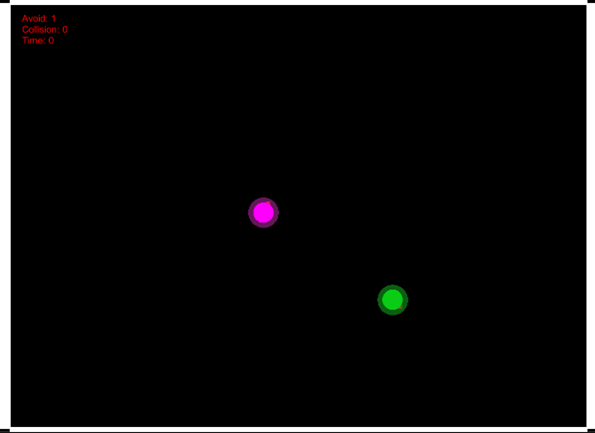
\includegraphics[width=0.9\textwidth]{Pictures/two users share real space.png}%imagine location
% 	\caption{Simulation for two users.}\label{fig:Simulation_2}%use name for ref.
	
% \end{figure}


% \begin{figure}[H]\centering
% 	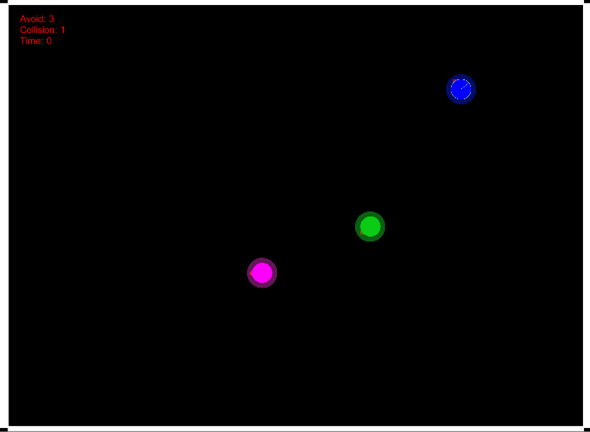
\includegraphics[width=0.9\textwidth]{Pictures/three users share real space.png}%imagine location
% 	\caption{Simulation for three users.}\label{fig:Simulation_3}%use name for ref.
	
% \end{figure}


% \begin{figure}[H]\centering
% 	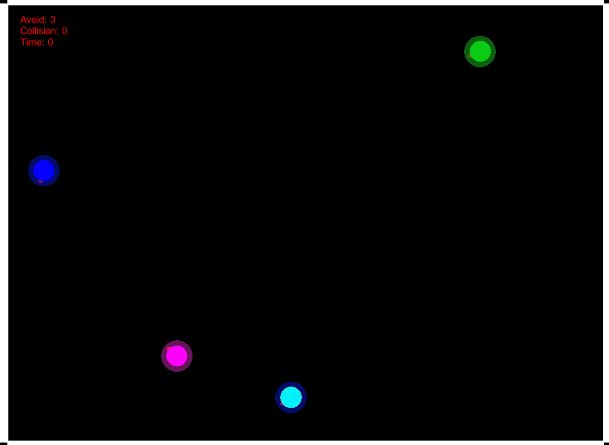
\includegraphics[width=0.9\textwidth]{Pictures/four users share real space.png}%imagine location
% 	\caption{Simulation for four users.}\label{fig:Simulation_4}%use name for ref.
	
% \end{figure}


% \begin{figure}[H]\centering
% 	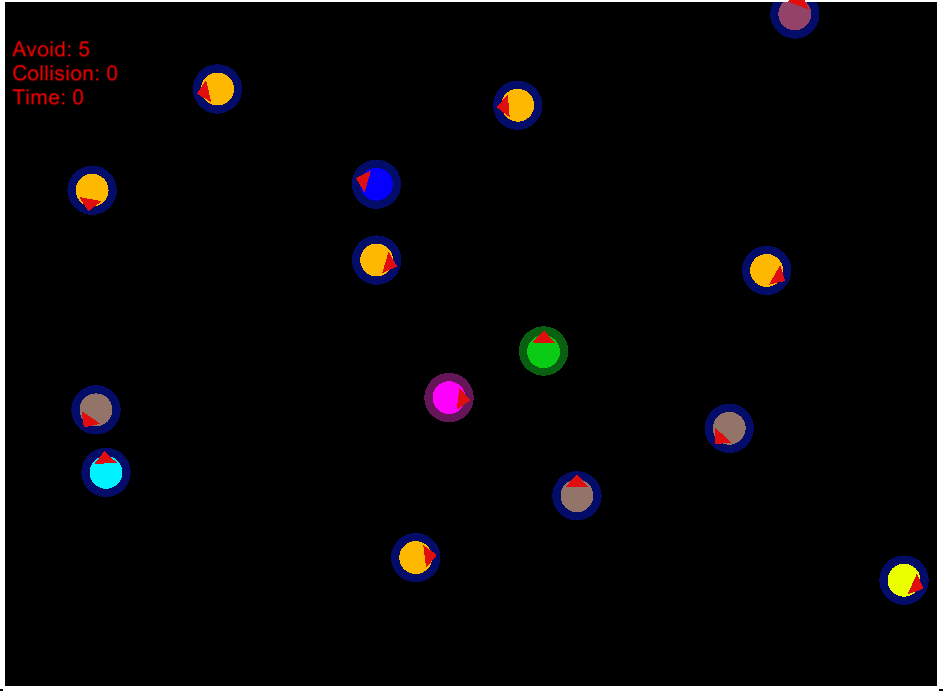
\includegraphics[width=0.9\textwidth]{Pictures/fifteen users share real space.png}%imagine location
% 	\caption{Simulation for fifteen users.}\label{fig:Simulation_15}%use name for ref.
	
% \end{figure}

% \newpage

% \begin{table}[h!]\centering
% 	\caption{Data Collection.}
% 	\label{tab:Data CollectionEx3}%\scriptsize
% 		\scalebox{1.0}{
% 	\begin{tabular}{ |p{4cm}|p{3cm}|p{6cm}|}
% 	\hline
% 		Variable & Unit & Description \\\hline
% 		Count of avoidance & count &Number of occasions that a collision with other agents are successfully avoided.\\\hline
% 		Count of collision & count & Number of collisions with other agents that occur during the trial.\\\hline
		
		
% 	\end{tabular}
% 	}
% \end{table} 

%  A series of simulation is conducted under the following conditions. 14 patterns of agents (2$\sim$15) x 3 physical areas (Large, Medium and Small) x 10 trials x 2 methods = 840 trials in all. The data to be collected during each trial is summarised in Table.~\ref{tab:Data CollectionEx3}.

% \newpage

% \section{Results}
% Fig.~\ref{fig:Area of 75 Percent} to Fig.~\ref{fig:Area of 125 Percent} show both the count of collisions and count of avoidance. The horizontal axis is the number of agents and the vertical one is the number of counts. The red line shows data from the Holm's method and the blue line shows data from the proposed method. The dash line is the count of collisions and the solid line is the count of avoidance. The three figures draw those lines at each different size of physical areas: Small, Medium and Large. From the results, it seems that as the area is larger, the counts of collisions and avoidance are reduced. Additionally, across all the number of agents for all the size of physical areas, the count of collisions for the proposed method is lower than the Holm's one.


% Fig.~\ref{fig:Performance of the number of collisions} and Fig.~\ref{fig:Performance Averages} show a comparative improvement of the proposed method to the Holm's method. The horizontal axis is the number of agents and the vertical one is the percentage of the count of collisions from the proposed method for the one from the Holm's method at each different size of area (if the percentage is 100 percent, it means no improvement.) At Large area, an average of ratio is 80.22 percent. Fig.~\ref{fig:Performance Averages} shows the average and its standard deviation across all the number of agents at each different size of area.

% Fig.~\ref{fig:Average of count of collisions} shows the average of counts of collisions at each different size of area for each method across all the number of agents. From the graph, there is a significant difference in the count of collisions between the Holm's method and proposed one for Medium and Large areas.  Fig.~\ref{fig:Average of count of collisions avoidance} shows the average of counts of avoidance at each different size of area for each method across all the number of agents. From the graph,  there is a significant difference in the count of  avoidance between the two methods for all the sizes of areas. The details of statistical evaluation are found in Appendix \ref{appendix:d} and Appendix \ref{appendix:e}.

% Fig.~\ref{fig:Collision times average in all areas of our method} shows the average of counts of collisions at each the number of agents for each method across different sizes of areas. The count of collisions decreases after applying the proposed method over all the number of agents.  Fig.~\ref{fig:Avoidance times average in all areas of our method} indicates the average of counts of avoidance at each the number of agents for each method, the agents can avoid collisions better by 44.37\% in comparison with the Holm's method.

% \newpage

% \begin{figure}[H]\centering
% 	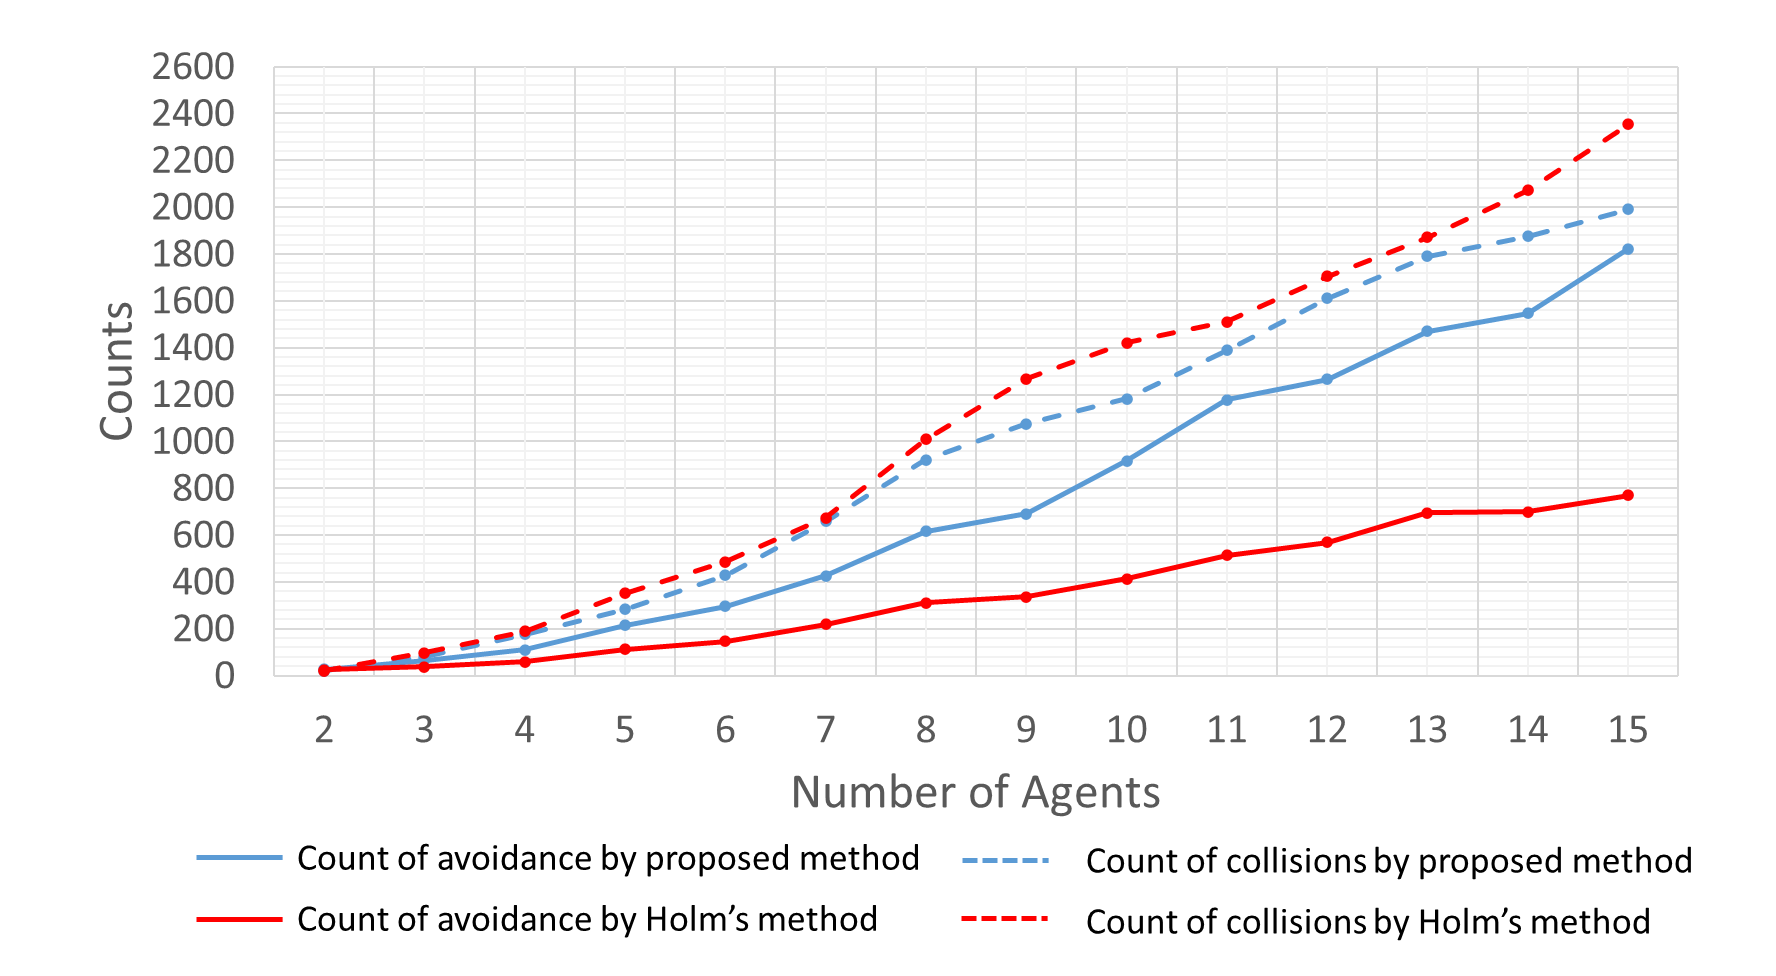
\includegraphics[width=1.0\textwidth]{Pictures/Area of 75 Percent.png}%imagine location
% 	\caption{Performance of collision avoidance for Small area.}\label{fig:Area of 75 Percent}%use name for ref.
	
% \end{figure}

% \begin{figure}[H]\centering
% 	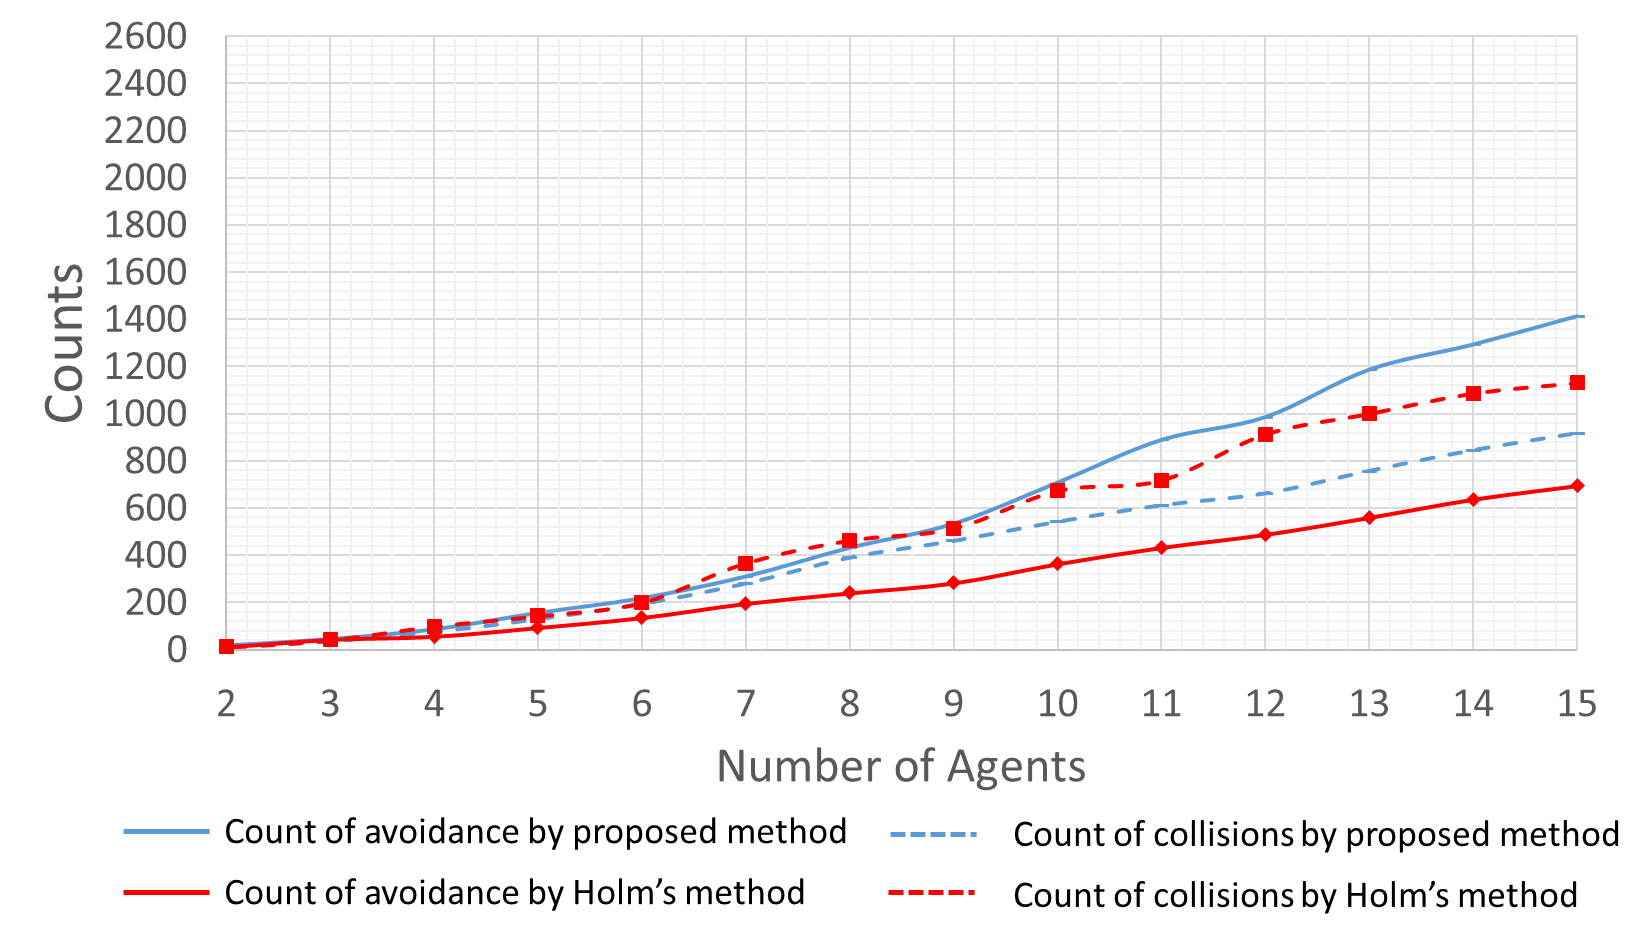
\includegraphics[width=1.0\textwidth]{Pictures/Area of 100 Percent.png}%imagine location
% 	\caption{Performance of collision avoidance for Medium area.}\label{fig:Area of 100 Percent}%use name for ref.
	
% \end{figure}

% \begin{figure}[H]\centering
% 	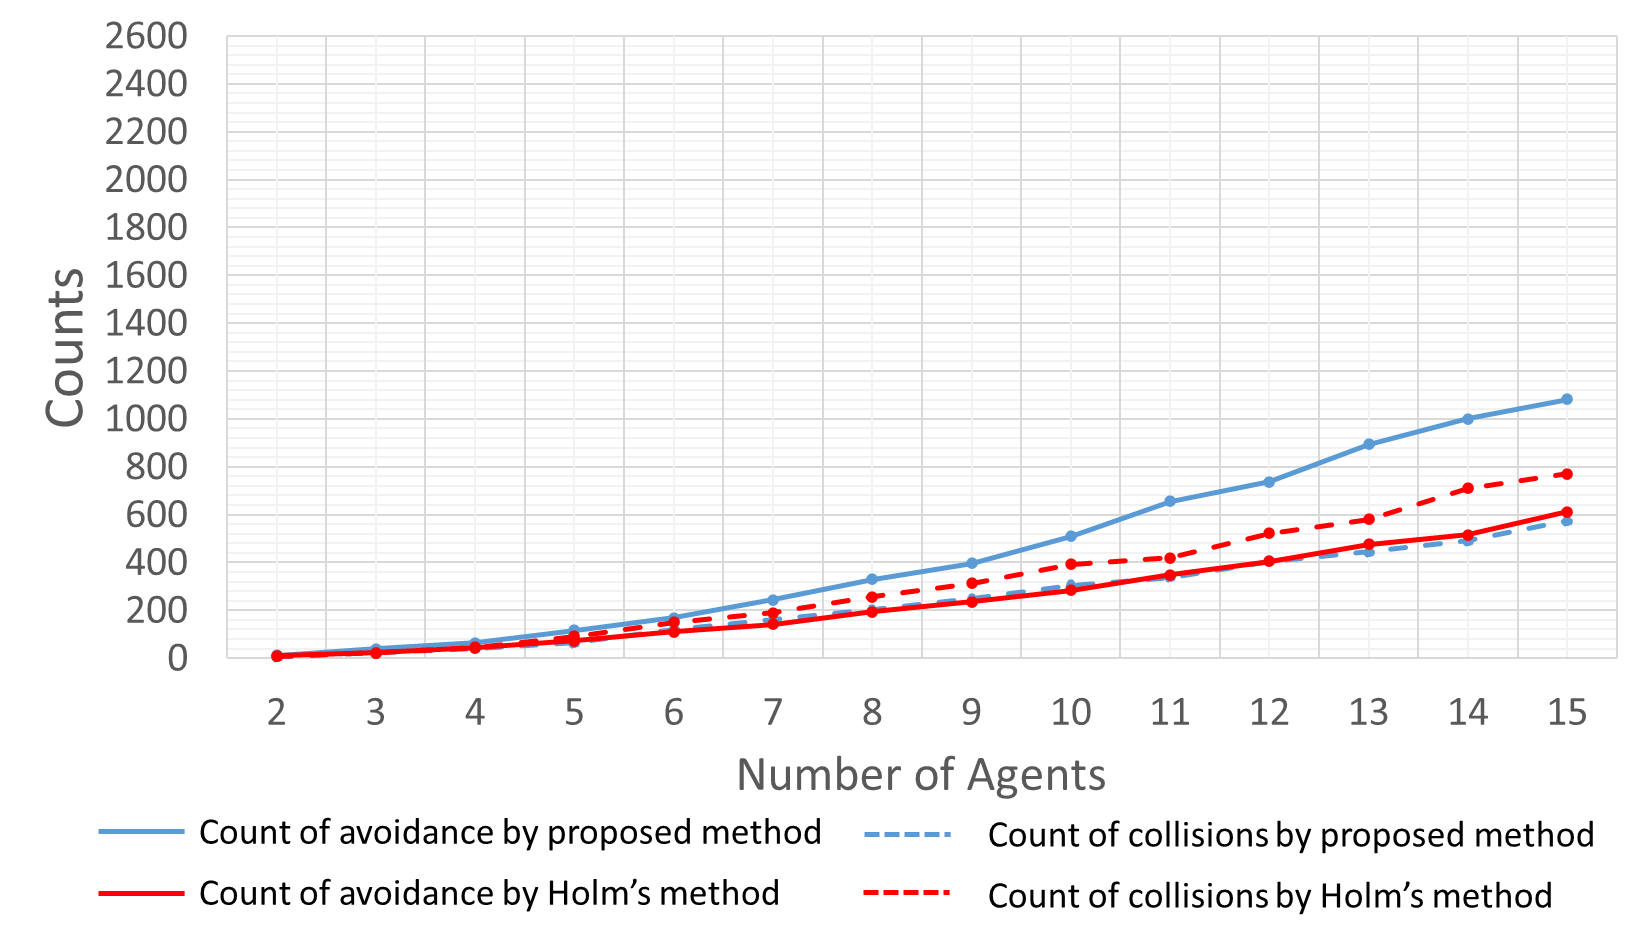
\includegraphics[width=1.0\textwidth]{Pictures/Area of 125 Percent.png}%imagine location
% 	\caption{Performance of collision avoidance for Large area.}\label{fig:Area of 125 Percent}%use name for ref.
	
% \end{figure}
% \newpage
% \begin{figure}[H]\centering
% 	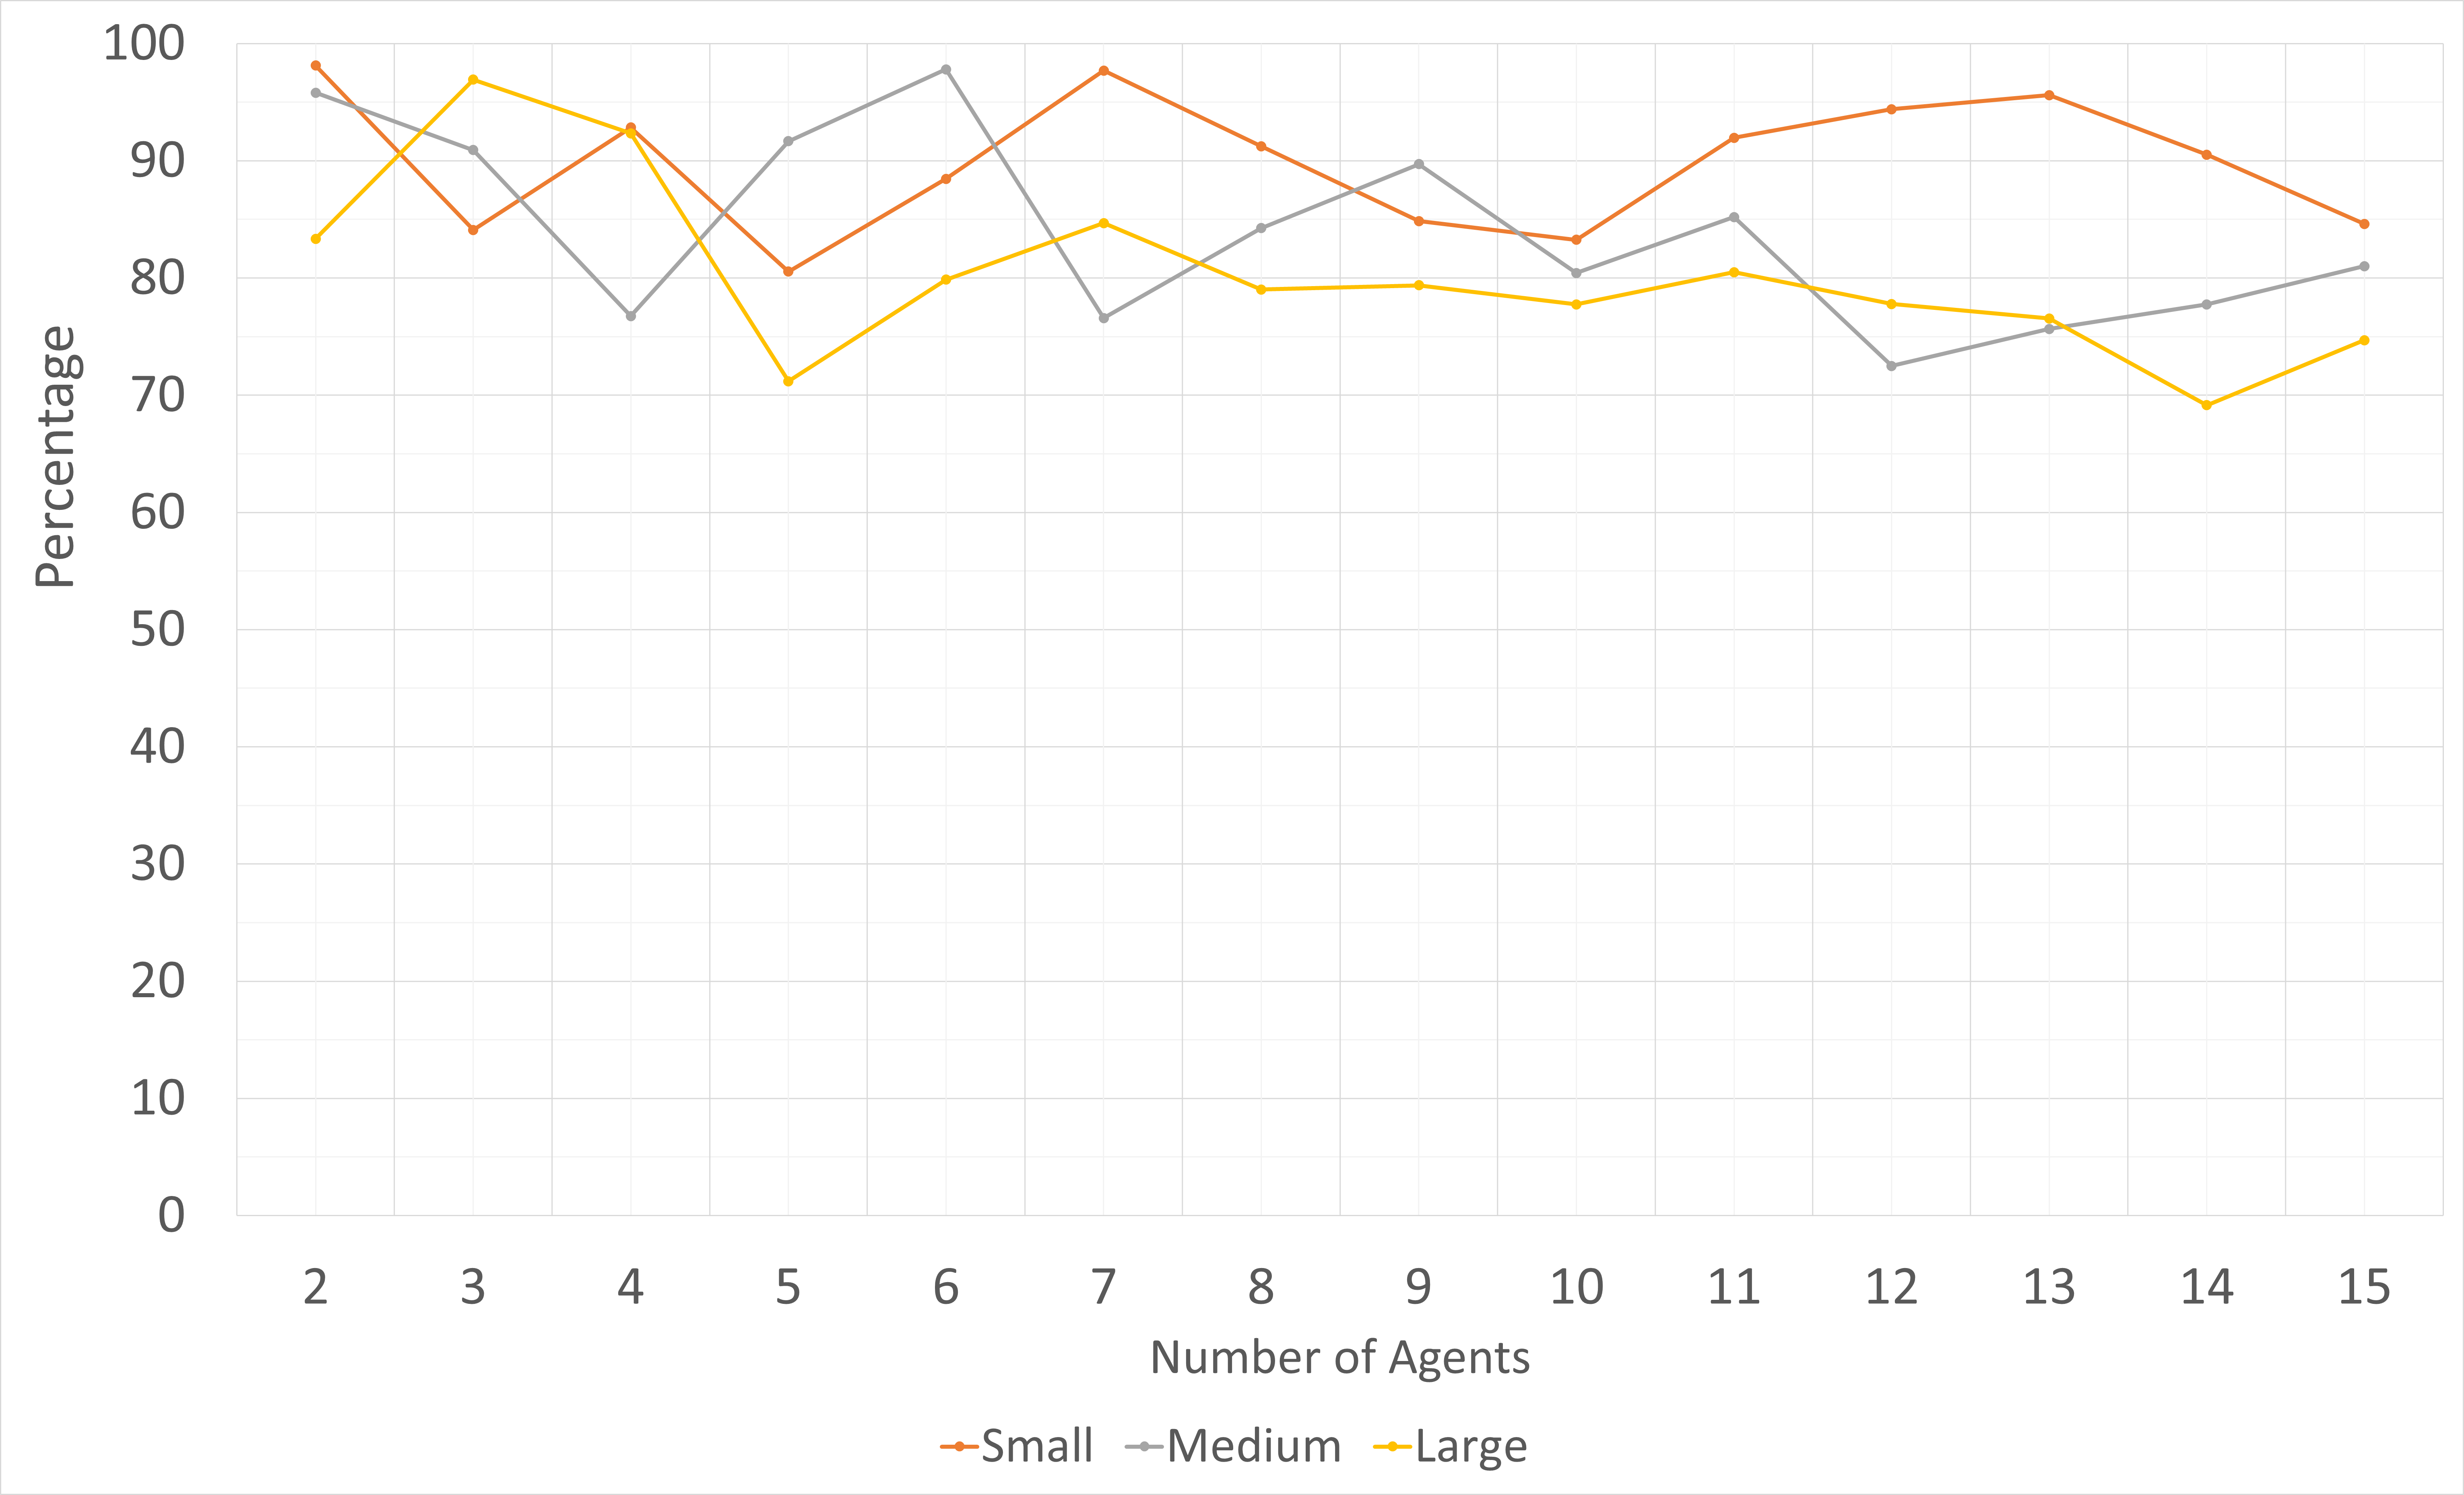
\includegraphics[width=1.0\textwidth]{Pictures/Performance of the number of collisions.png}%imagine location
% 	\caption{Improvement of the proposed method for the Holm's method in terms of the count of collisions.}\label{fig:Performance of the number of collisions}%use name for ref.
	
% \end{figure}
% \begin{figure}[H]\centering
% 	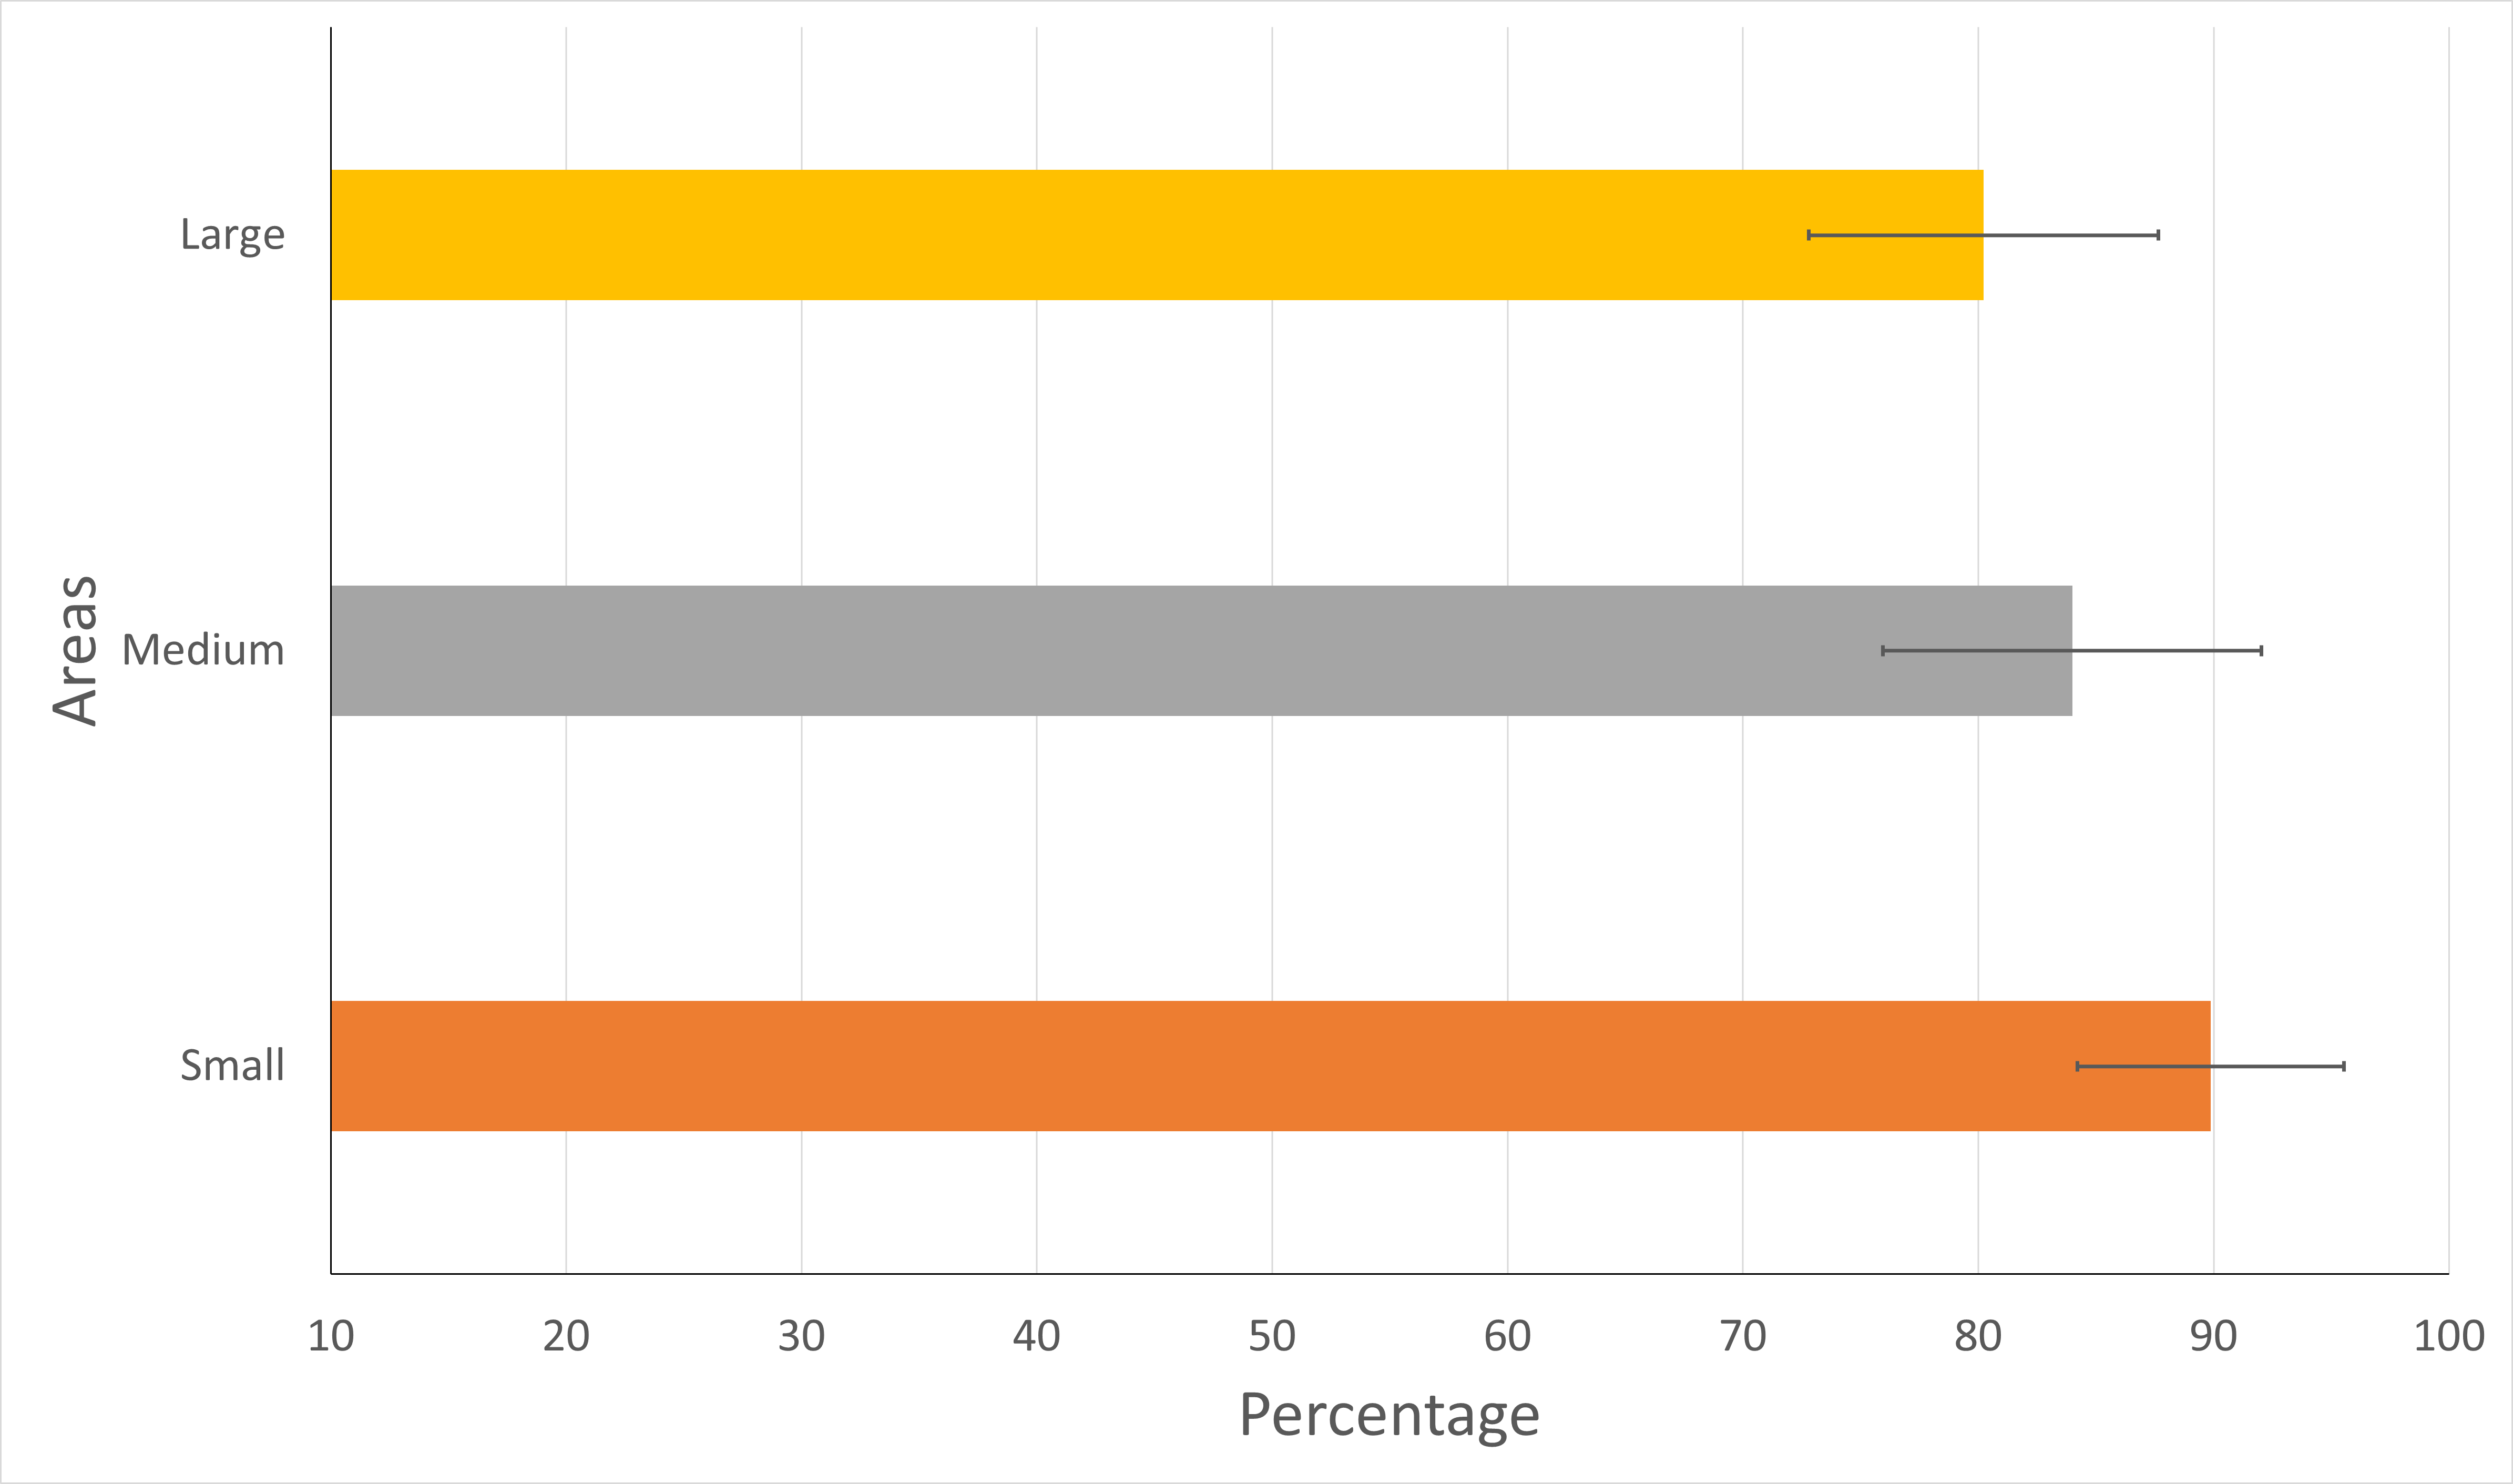
\includegraphics[width=1.0\textwidth]{Pictures/Performance Averages.png}%imagine location
% 	\caption{Average of the improvement.}\label{fig:Performance Averages}%use name for ref.
	
% \end{figure}


% \begin{figure}[H]\centering
% 	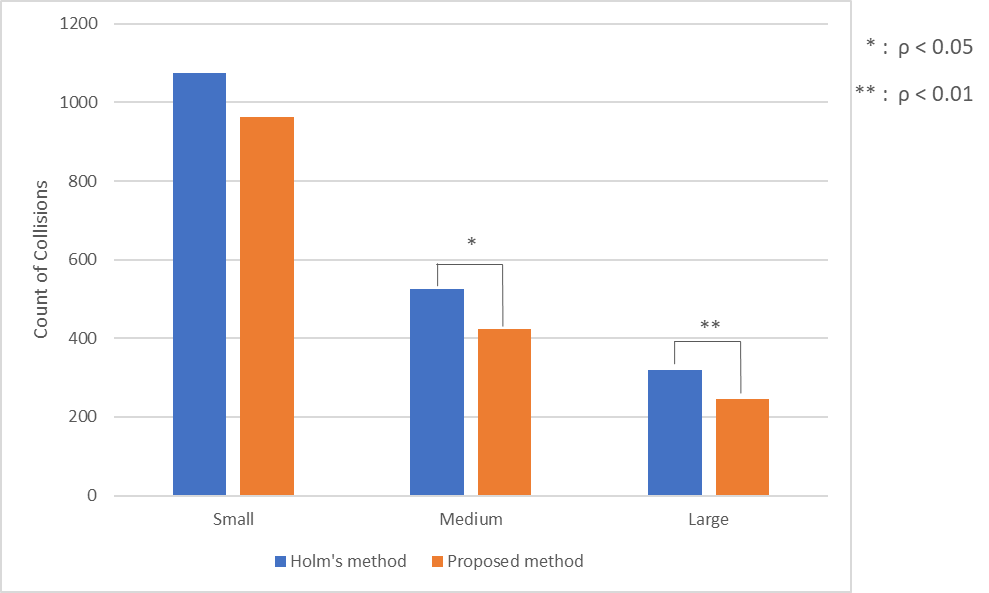
\includegraphics[width=1.0\textwidth]{Pictures/Average of count of collisions of each different of area.png}%imagine location
% 	\caption{Average of counts of collisions at each different size of area.}\label{fig:Average of count of collisions}%use name for ref.
	
% \end{figure}
% \begin{figure}[H]\centering
% 	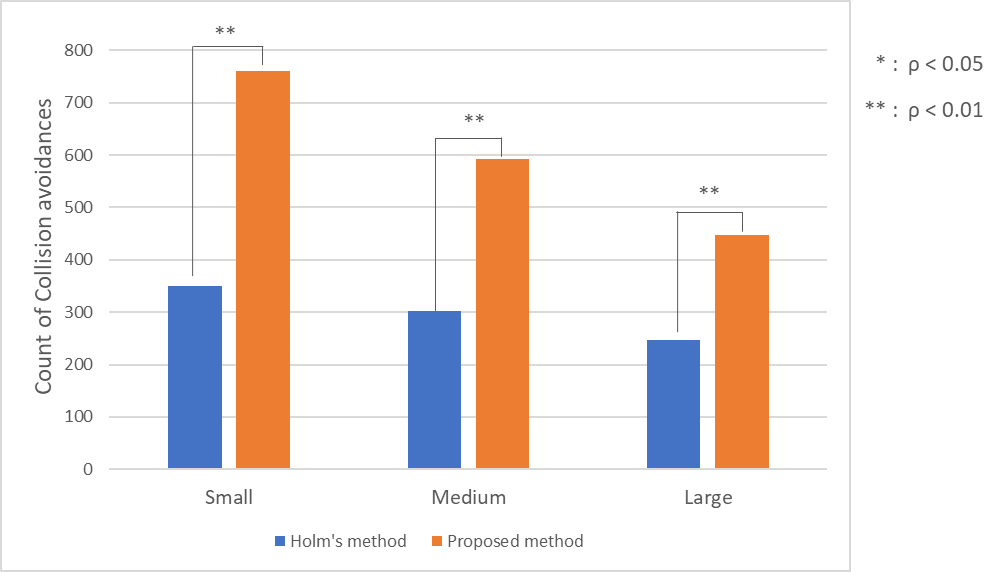
\includegraphics[width=1.0\textwidth]{Pictures/Average of count of avoidance of each different of area.png}%imagine location
% 	\caption{Average of counts of avoidance at each different size of area.}\label{fig:Average of count of collisions avoidance}%use name for ref.
	
% \end{figure}
% %\newpage




% \begin{figure}[H]\centering
% 	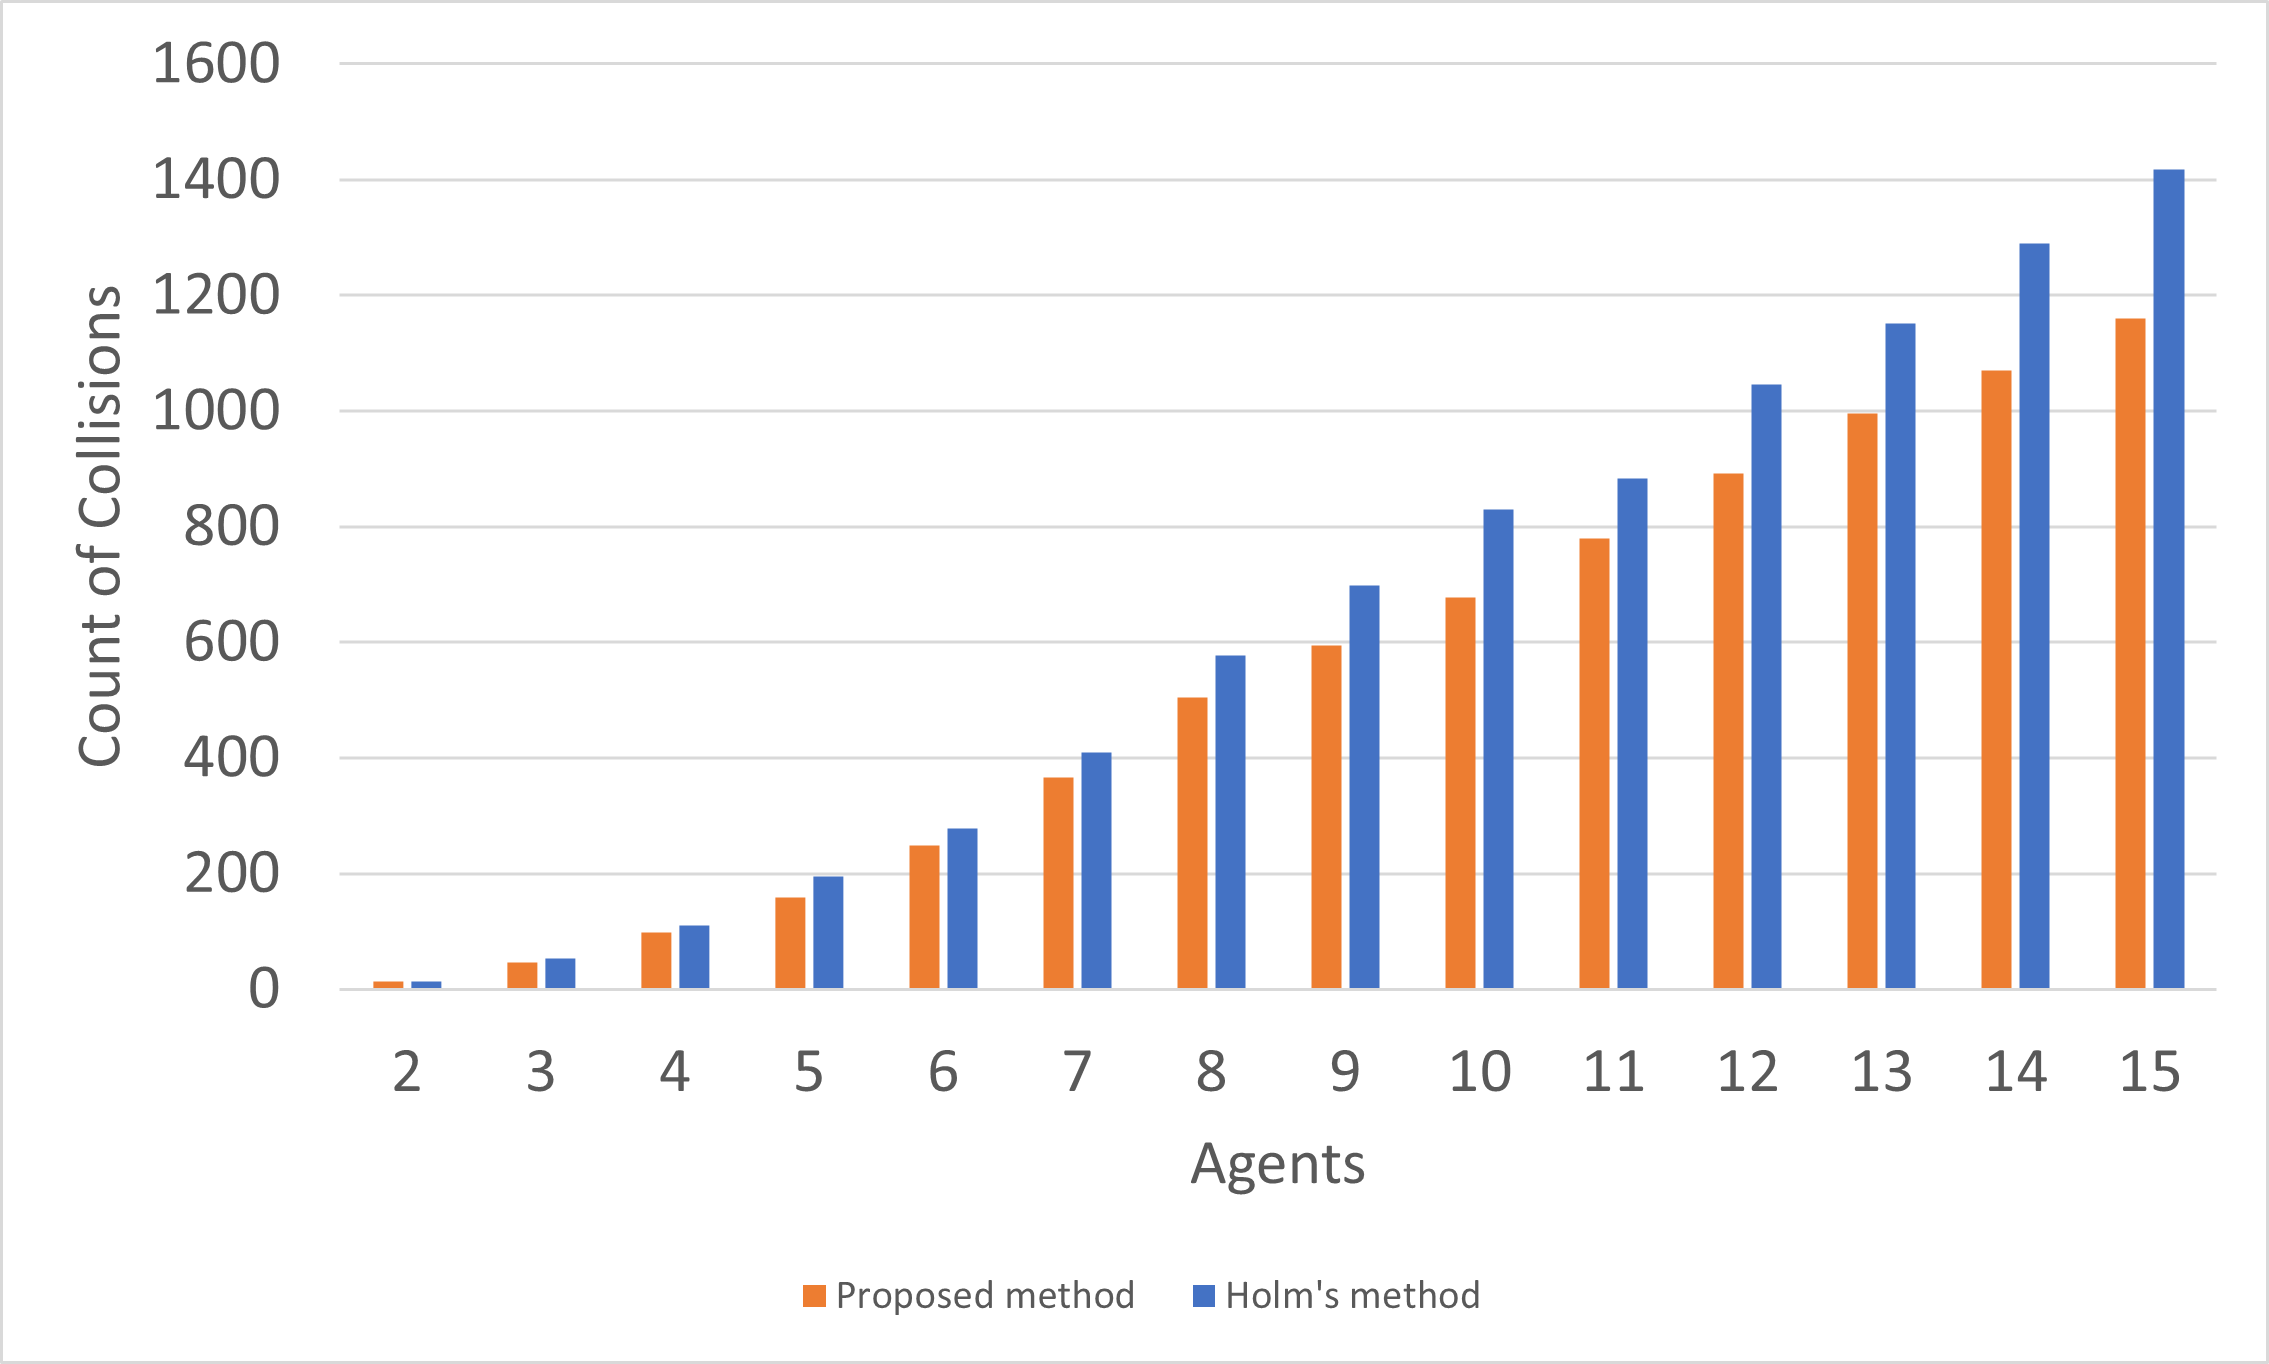
\includegraphics[width=1.0\textwidth]{Pictures/Average of count of collision of across all the number of user.png}%imagine location
% 	\caption{Average of counts of collisions at each the number of agents for each method.}\label{fig:Collision times average in all areas of our method}%use name for ref.
	
% \end{figure}
% \begin{figure}[H]\centering
% 	\includegraphics[width=1.0\textwidth]{Pictures/Average of count of collision avoidance of across all the number of user.png}%imagine location
% 	\caption{Average of counts of avoidance at each the number of agents for each method.}\label{fig:Avoidance times average in all areas of our method}%use name for ref.
	
% \end{figure}





\chapter{Discussion} % Main chapter title

\label{Chapter5} % Change X to a consecutive number; for referencing this chapter elsewhere, use \ref{ChapterX}


%----------------------------------------------------------------------------------------
%	SECTION 1
%----------------------------------------------------------------------------------------
When an HMD is deployed, users struggle to understand their surroundings, identify their orientation and determine where they are in relation to other objects such as walls and users in their physical space. 
In consideration of this, it is highly likely that users wearing HMDs collide with other users and walls. 

To resolve this problem, the proposed method employs a strategy with a time-dependent synced-rotational gain to avoid collisions between multiple VR users sharing the same physical space. The results mentioned in the previous chapter prove that the proposed method works better than the Holm's one. This chapter describes some concerns that would affect the results. 
\section{Motion sickness}
From Fig.~\ref{fig:SSQ_CtoS_Of_RorationEx} to Fig.~\ref{fig:SSQ_Acc_Of_RotationEx} on rotation awareness experiments, the subjects manifested symptoms at slight and moderate levels and they could continue the experiments.
From Fig.~\ref{fig:SSQ_ConstantOfCurvatureEx} and Fig.~\ref{fig:SSQ_AccOfCurvatureEx} on curvature distance experiments, two subjects from five subjects manifested symptoms in severe level. During the experiment on curvature distance, two of the five subjects started to have eye strain and difficulty in focusing the given task at the speed of rotation of 3.2deg/s. However, they said they could overcome motion sickness if they could take a break and then I temporarily suspended them for the extra rest time of five minutes. While they had a rest time, I recommended them to see the outside of the room such as trees and the nearby buildings. After that, their motion sickness had been reduced to a low level and they continued the task and did not experience motion sickness.

\begin{figure}[H]\centering
	\includegraphics[width=0.9\textwidth]{Pictures/SSQ_StoC_Of_RorationEx.png}%imagine location
	\caption{SSQ results for the stop to constant speed rotation task.}\label{fig:SSQ_StoC_Of_RorationEx}%use name for ref.
	
\end{figure}
\begin{figure}[H]\centering
	\includegraphics[width=0.9\textwidth]{Pictures/SSQ_CtoS_Of_RorationEx.png}%imagine location
	\caption{SSQ results for the constant speed to stop rotation task.}\label{fig:SSQ_CtoS_Of_RorationEx}%use name for ref.
	
\end{figure}
\begin{figure}[H]\centering
	\includegraphics[width=0.9\textwidth]{Pictures/SSQ_Dec_Of_RotationEx.png}%imagine location
	\caption{SSQ results for the deceleration rotation task.}\label{fig:SSQ_Dec_Of_RotationEx}%use name for ref.
	
\end{figure}
\begin{figure}[H]\centering
	\includegraphics[width=0.9\textwidth]{Pictures/SSQ_Acc_Of_RotationEx.png}%imagine location
	\caption{SSQ results for the acceleration rotation task.}\label{fig:SSQ_Acc_Of_RotationEx}%use name for ref.

\end{figure}
\begin{figure}[H]\centering
	\includegraphics[width=0.9\textwidth]{Pictures/SSQ_ConstantOfCurvatureEx.png}%imagine location
	\caption{SSQ results for the constant speed task.}\label{fig:SSQ_ConstantOfCurvatureEx}%use name for ref.
	
\end{figure}
\begin{figure}[H]\centering
	\includegraphics[width=0.9\textwidth]{Pictures/SSQ_AccOfCurvatureEx.png}%imagine location
	\caption{SSQ results for the acceleration task.}\label{fig:SSQ_AccOfCurvatureEx}%use name for ref.
	
\end{figure}
\section{Deployment in the real scenario}
From the simulation result, collisions can be avoided efficiently by the proposed method. However, when the proposed method is applied to the real scenario, there should be room for discussion. The simulation of the proposed method has a restricted condition that is the speed of walking 0.5m/s. If it is more or less than 0.5 m/s, the collision avoidance would be possible to fail and the collision possibility would be high. The further experiment on the relation between the speed of walking, the speed of rotation, and curvature distance, are needed. 
\section{Shapes of physical spaces}
The proposed method was evaluated by simulation where the physical space was a rectangular room. Three sizes of physical spaces were taken into consideration: Large, Medium and Small. In the real scenario, there must be tables, bookshelves, sofas, etc. in a room, leading to a complicated walking space. It has an effect on the collision possibility. A further experiment on the relation between practical layouts of a room and performance of collision avoidance is needed. 
\section{Effect of simulation frame rate on collision prediction}
The simulation ran on the Unity engine in the experiment. In Unity, to advance the simulation each step, Update() function is called to change properties of objects before they are rendered at each frame. The interval between Update() calls varies depending on an amount of rendering loads. If the interval slowed down, the collision prediction would not work properly. Because each agent walks at the speed of 0.5m/s, the distance he/she travels between frames is 0.83cm when the frame rate is 60 frames per second or fps. Fig.~\ref{fig:framerate} shows the relation between frame rates and the number of agents. The lowest frame rate is 51.13629 and the distance each agent travels between frames is 0.978cm in that case. This frame rate is expected not to affect the collision prediction.
%For testing the first experiment, we had a subject (5 people) and gave them to wear and try to notice the rotation in the virtual environment. We discussed and recorded the time for subjects to notice the rotation speed of (0.4deg/s, 0.8deg/s, 1.6deg/s, 3.2deg/s, 6.4deg/s and 12.8deg/s) when stop to constant speed and constant speed to stop rotation. In additional, we recorded the time for subjects to notice the deceleration and acceleration of (33\%, 66\% and 100\%) and the max rotation speeds are 0.4deg/s, 0.8deg/s, 1.6deg/s and 3.2deg/s. We knew the notice time of users, but we did not know about the rerated of a virtual environment and physical space distance in user moving situations. Also, while the user is walking the scene that we created in the program and we need them to rotate to make the curvature distance to avoid a collision with other users. We had to consider the average of half the width of a human shoulder (23cm) that affects the user's moving to avoid a collision with other users. So, we did another experiment that let the subject walk in a virtual environment and measured the distances in the constant speed task and acceleration task.
%From the result of both experiments, we had enough of the actual situation's information to make the simulation for multiple users (2 to 15). Based on the previous experiments' data, we create the simulation that the colliding users will be rotated while walking to avoid the collision when the collision is detected. When more than two users collide, all of the colliding users will be rotated. From the discussion, we need to know the proposed method's efficiency, and then we find the other method for comparing. We found that Holm's method is often used to avoid collisions between users. Then, we create Holm's method simulation. As more than two users share a physical place, we concluded that the proposed method is better compared to Holm's way because when three or more users have predicted a collision at the same time, Holm's method can be enabled collision avoidance function for only even number of users. When the number of users becomes an odd number, Holm's method can not notice some users and fail to collision avoidance, but the proposed method can enable a collision avoidance function that can be predicted for a collision of multiple users. Also, the proposed method's count of collision is lower than Holm's method and the count of successful avoidance is higher than Holm's method.
\begin{figure}[H]\centering
	\includegraphics[width=1.0\textwidth]{Pictures/framerate.png}%imagine location
	\caption{Average of frame rate at each the number of agents.}\label{fig:framerate}%use name for ref.
	
\end{figure}
\chapter{Conclusion} % Main chapter title

\label{Chapter6}

This study investigated methods to enhance immersion in virtual reality experiences through the development of a wearable haptic glove. The glove is equipped with flex sensors, an IMU (MPU-6050), and a coin-type vibration motor. I utilized PWM-based vibrotactile feedback to examine participants' ability to differentiate between various vibration cycle rates and to assess how these tactile signals influenced the perceived realism of virtual textures.

In two structured experiments, the results indicated that participants could reliably distinguish between textures based on their smoothness. Higher accuracy was observed at higher cycle rates, especially when identifying differences among textures with varying levels of roughness. Subjective evaluations were analyzed using Wilcoxon Signed-Rank tests on composite category scores, revealing a statistically significant improvement in the category of `Realistic and Aligned Tactile Sensations Felt.' However, perceptions related to the categories of `Hand Ownership and Control' and `Immersion,' while often showing favorable trends, did not reach statistical significance when compared to a neutral baseline. A significant factor contributing to these challenges, as highlighted by participant feedback, was the poor fit of the fixed-size glove.

Building on these findings, future work will focus on optimizing feedback parameters, such as vibration cycle rates and duty cycles, to achieve more accurate and nuanced texture rendering. Additionally, the system will be expanded to include a wider variety of virtual textures, enhancing realism across different surface types. 

Furthermore, I will increase the number of participants in subsequent experiments to improve the statistical robustness and generalizability of the results. I also aim to implement adaptive feedback algorithms capable of dynamically adjusting haptic parameters based on real-time user interactions, thereby further enhancing the immersion and interactivity of VR applications.





 

\begin{acknowledgements}
\addchaptertocentry{\acknowledgementname} % Add the acknowledgements to the table of contents
%
I would like to express my deep gratitude to Professor Makio Ishihara for his invaluable guidance, continuous support, and encouragement throughout my research journey. I am also very thankful to all the students in the Ishihara Laboratory for their cooperation and participation in the experiments, as well as for their helpful discussions and technical assistance.

\vspace{+0.5cm}
My sincere thanks go to all the administrative staff at FIT who have provided constant support since the beginning of my academic journey. I would especially like to thank Ms. Kono Akiko for her dedicated instruction in the Japanese language and her thoughtful support in various aspects of daily life.

\vspace{+0.5cm}
Finally, I wish to express my heartfelt appreciation to all members of FBK for their kindness, valuable advice, and enthusiastic encouragement, which have significantly enriched my study experience in Japan.

\end{acknowledgements}




%----------------------------------------------------------------------------------------
%	THESIS CONTENT - APPENDICES
%----------------------------------------------------------------------------------------

%\appendix % Cue to tell LaTeX that the following "chapters" are Appendices

% Include the appendices of the thesis as separate files from the Appendices folder
% Uncomment the lines as you write the Appendices

%\include{Appendices/AppendixA}
%\include{Appendices/AppendixB}
%\include{Appendices/AppendixC}

%----------------------------------------------------------------------------------------
%	BIBLIOGRAPHY
%----------------------------------------------------------------------------------------
%\bibliographystyle{ieeetr}
\printbibliography[heading=bibintoc, title={References}]
%\bibliography{bibliography}
%\nocite{*}
\cleardoublepage
%----------------------------------------------------------------------------------------
%	Publications
%----------------------------------------------------------------------------------------
\appendix
\addchap{List of Papers}
\label{ap:research_list}



%?��.国際会議  21件?��うち第1著�?7編、�?�著�?14編?�?
%
%�?第一著�?

\addsec{International Conference Papers}
	\begin{enumerate}
		\bibitem[20]{ieice} K. Witchuvanit, M. Ishihara, ``Wearable Haptic Feedback Glove for Texture Rendering in Virtual Reality,'' Proc. of The 19-th International Conference on Complex, Intelligent, and Software Intensive Systems 2025, July 2025.
	\end{enumerate}
	
	

\begin{appendices}
    % A1
\chapter{Experiment 1's Answers Tables}
\label{appendix:a}
1 is 0.2 cycle, 2 is 0.5 cycle, 3 is 1.0 cycle
%%%%%%%%%%%%%%%%%%%%collision  F & t-Test%%
%%%%%%%%%%%%%%%%%%%%%75per
% \begin{table}[H]\centering
%   \caption{Material and Smoothness}
%     \begin{tabular}{ p{3cm}|p{5cm}|p{5cm}}
%     \toprule
%     \textbf{Material} & \multicolumn{1}{l|}{\textbf{Smoothness}} \\
%     \midrule
%     Brick & 1 \\
%     \midrule
%     Grass & 2 \\
%     \midrule
%     Marble & 3 \\
%     \bottomrule
%     \end{tabular}%
%   \label{tab:addlabel}%
% \end{table}%
% Table generated by Excel2LaTeX from sheet '1st'
\begin{table}[H]
  \centering
  \caption{First participants' answers to the first experiment.}
    \begin{tabular}{|r|r|}
    \toprule
    \multicolumn{1}{|l|}{\textbf{Real}} & \multicolumn{1}{l|}{\textbf{Answer}} \\
    \midrule
    1     & 1 \\
    \midrule
    3     & 3 \\
    \midrule
    2     & 1 \\
    \midrule
    3     & 3 \\
    \midrule
    2     & 2 \\
    \midrule
    1     & 1 \\
    \midrule
    1     & 2 \\
    \midrule
    2     & 2 \\
    \midrule
    2     & 2 \\
    \midrule
    2     & 2 \\
    \midrule
    3     & 3 \\
    \midrule
    1     & 1 \\
    \midrule
    3     & 3 \\
    \midrule
    3     & 3 \\
    \midrule
    1     & 1 \\
    \bottomrule
    \end{tabular}%
  \label{tab:Ex1_1}%
\end{table}%

% Table generated by Excel2LaTeX from sheet '2nd'
\begin{table}[H]
  \centering
  \caption{Second participants' answers to the first experiment.}
    \begin{tabular}{|r|r|}
    \toprule
    \multicolumn{1}{|l|}{Real} & \multicolumn{1}{l|}{Answer} \\
    \midrule
    2     & 2 \\
    \midrule
    3     & 3 \\
    \midrule
    3     & 3 \\
    \midrule
    1     & 1 \\
    \midrule
    3     & 2 \\
    \midrule
    1     & 1 \\
    \midrule
    2     & 2 \\
    \midrule
    2     & 2 \\
    \midrule
    2     & 1 \\
    \midrule
    1     & 2 \\
    \midrule
    1     & 1 \\
    \midrule
    2     & 2 \\
    \midrule
    3     & 3 \\
    \midrule
    3     & 3 \\
    \midrule
    1     & 1 \\
    \bottomrule
    \end{tabular}%
  \label{tab:Ex1_2}%
\end{table}%

% Table generated by Excel2LaTeX from sheet '3rd'
\begin{table}[H]
  \centering
  \caption{Third participants' answers to the first experiment.}
    \begin{tabular}{|r|r|}
    \toprule
    \multicolumn{1}{|l|}{Real} & \multicolumn{1}{l|}{Answer} \\
    \midrule
    3     & 3 \\
    \midrule
    1     & 1 \\
    \midrule
    2     & 2 \\
    \midrule
    2     & 2 \\
    \midrule
    3     & 3 \\
    \midrule
    3     & 3 \\
    \midrule
    1     & 1 \\
    \midrule
    1     & 1 \\
    \midrule
    2     & 1 \\
    \midrule
    1     & 1 \\
    \midrule
    2     & 1 \\
    \midrule
    3     & 2 \\
    \midrule
    3     & 3 \\
    \midrule
    1     & 2 \\
    \midrule
    2     & 2 \\
    \bottomrule
    \end{tabular}%
  \label{tab:Ex1_3}%
\end{table}%

% Table generated by Excel2LaTeX from sheet '4th'
\begin{table}[H]
  \centering
  \caption{Fourth participants' answers to the first experiment.}
    \begin{tabular}{|r|r|}
    \toprule
    \multicolumn{1}{|l|}{Real} & \multicolumn{1}{l|}{Answer} \\
    \midrule
    3     & 3 \\
    \midrule
    3     & 3 \\
    \midrule
    3     & 3 \\
    \midrule
    1     & 1 \\
    \midrule
    1     & 1 \\
    \midrule
    1     & 1 \\
    \midrule
    1     & 2 \\
    \midrule
    2     & 2 \\
    \midrule
    1     & 2 \\
    \midrule
    2     & 2 \\
    \midrule
    3     & 3 \\
    \midrule
    3     & 3 \\
    \midrule
    2     & 2 \\
    \midrule
    2     & 1 \\
    \midrule
    2     & 2 \\
    \bottomrule
    \end{tabular}%
  \label{tab:Ex1_4}%
\end{table}%

% Table generated by Excel2LaTeX from sheet '5th'
\begin{table}[H]
  \centering
  \caption{Fifth participants' answers to the first experiment.}
    \begin{tabular}{|r|r|}
    \toprule
    \multicolumn{1}{|l|}{Real} & \multicolumn{1}{l|}{Answer} \\
    \midrule
    3     & 3 \\
    \midrule
    3     & 3 \\
    \midrule
    1     & 1 \\
    \midrule
    1     & 1 \\
    \midrule
    1     & 2 \\
    \midrule
    3     & 3 \\
    \midrule
    2     & 1 \\
    \midrule
    2     & 2 \\
    \midrule
    1     & 1 \\
    \midrule
    2     & 2 \\
    \midrule
    3     & 3 \\
    \midrule
    1     & 1 \\
    \midrule
    2     & 2 \\
    \midrule
    3     & 3 \\
    \midrule
    2     & 2 \\
    \bottomrule
    \end{tabular}%
  \label{tab:Ex1_5}%
\end{table}%

% Table generated by Excel2LaTeX from sheet '6th'
\begin{table}[H]
  \centering
  \caption{Sixth participants' answers to the first experiment.}
    \begin{tabular}{|r|r|}
    \toprule
    \multicolumn{1}{|l|}{Real} & \multicolumn{1}{l|}{Answer} \\
    \midrule
    1     & 2 \\
    \midrule
    2     & 2 \\
    \midrule
    1     & 1 \\
    \midrule
    3     & 3 \\
    \midrule
    3     & 2 \\
    \midrule
    3     & 3 \\
    \midrule
    2     & 2 \\
    \midrule
    2     & 2 \\
    \midrule
    3     & 3 \\
    \midrule
    2     & 2 \\
    \midrule
    1     & 1 \\
    \midrule
    3     & 2 \\
    \midrule
    1     & 1 \\
    \midrule
    2     & 2 \\
    \midrule
    1     & 1 \\
    \bottomrule
    \end{tabular}%
  \label{tab:Ex1_6}%
\end{table}%

\chapter{Experiment 2's Answers Tables}
\label{appendix:b}
1 is 0.2 cycle, 2 is 0.5 cycle, 3 is 1.0 cycle
% Table generated by Excel2LaTeX from sheet '1st'
\begin{table}[H]
  \centering
  \caption{First participants' answers to the second experiment.}
    \begin{tabular}{|l|r|}
    \toprule
    \textbf{Material} & \multicolumn{1}{l|}{\textbf{Smoothness}} \\
    \midrule
    Brick & 1 \\
    \midrule
    Grass & 2 \\
    \midrule
    Marble & 3 \\
    \bottomrule
    \end{tabular}%
  \label{tab:Ex2_1}%
\end{table}%

% Table generated by Excel2LaTeX from sheet '2nd'
\begin{table}[H]
  \centering
  \caption{Second participants' answers to the second experiment.}
    \begin{tabular}{|l|r|}
    \toprule
    \textbf{Material} & \multicolumn{1}{l|}{\textbf{Smoothness}} \\
    \midrule
    Brick & 1 \\
    \midrule
    Grass & 2 \\
    \midrule
    Marble & 3 \\
    \bottomrule
    \end{tabular}%
  \label{tab:Ex2_2}%
\end{table}%

% Table generated by Excel2LaTeX from sheet '3rd'
\begin{table}[H]
  \centering
  \caption{Third participants' answers to the second experiment.}
    \begin{tabular}{|l|r|}
    \toprule
    \textbf{Material} & \multicolumn{1}{l|}{\textbf{Smoothness}} \\
    \midrule
    Brick & 2 \\
    \midrule
    Grass & 1 \\
    \midrule
    Marble & 3 \\
    \bottomrule
    \end{tabular}%
  \label{tab:Ex2_3}%
\end{table}%

% Table generated by Excel2LaTeX from sheet '4th'
\begin{table}[H]
  \centering
  \caption{Fourth participants' answers to the second experiment.}
    \begin{tabular}{|l|r|}
    \toprule
    \textbf{Material} & \multicolumn{1}{l|}{\textbf{Smoothness}} \\
    \midrule
    Brick & 2 \\
    \midrule
    Grass & 2 \\
    \midrule
    Marble & 3 \\
    \bottomrule
    \end{tabular}%
  \label{tab:Ex2_4}%
\end{table}%

% Table generated by Excel2LaTeX from sheet '5th'
\begin{table}[H]
  \centering
  \caption{Fifth participants' answers to the second experiment.}
    \begin{tabular}{|l|r|}
    \toprule
    \textbf{Material} & \multicolumn{1}{l|}{\textbf{Smoothness}} \\
    \midrule
    Brick & 1 \\
    \midrule
    Grass & 2 \\
    \midrule
    Marble & 3 \\
    \bottomrule
    \end{tabular}%
  \label{tab:Ex2_5}%
\end{table}%

% Table generated by Excel2LaTeX from sheet '6th'
\begin{table}[H]
  \centering
  \caption{Sixth participants' answers to the second experiment.}
    \begin{tabular}{|l|r|}
    \toprule
    \textbf{Material} & \multicolumn{1}{l|}{\textbf{Smoothness}} \\
    \midrule
    Brick & 2 \\
    \midrule
    Grass & 1 \\
    \midrule
    Marble & 3 \\
    \bottomrule
    \end{tabular}%
  \label{tab:Ex2_6}%
\end{table}%

\chapter{Questionnaire's Answers Tables}
\label{appendix:c}
% Table generated by Excel2LaTeX from sheet '1st'
\begin{table}[H]
  \centering
  \caption{First participants' answers to the questionnaire.}
    \begin{tabular}{|lrrrrrrrr|r|}
    \toprule
    \multicolumn{9}{c|}{\multirow{2}[2]{*}{\textbf{Question}}}            & \multicolumn{1}{c|}{\multirow{2}[2]{*}{\textbf{Score}}} \\
    \multicolumn{9}{c|}{}                                                 &  \\
    \midrule
    \multicolumn{9}{|l|}{I felt as if the virtual hands were my own.}     & 3 \\
    \midrule
    \multicolumn{9}{|l|}{I felt that the tactile sensations were caused by the virtual hand.} & 4 \\
    \midrule
    \multicolumn{9}{|l|}{I felt as if my hand were the virtual hand.}     & 3 \\
    \midrule
    \multicolumn{9}{|l|}{I felt like I was controlling the movement of the virtual hand.} & 5 \\
    \midrule
    \multicolumn{9}{|l|}{I felt as if the virtual hand was naturally connected to my body.} & 3 \\
    \midrule
    \multicolumn{9}{|l|}{The tactile sensations I perceived felt naturally aligned with the virtual hand.} & 5 \\
    \midrule
    \multicolumn{9}{|l|}{When I touched the virtual plane, I felt as if my real hand was also being touched.} & 5 \\
    \midrule
    \multicolumn{9}{|l|}{The movements of the virtual hand felt natural to me.} & 3 \\
    \midrule
    \multicolumn{9}{|l|}{I felt that the virtual hand responded as expected to my movements.} & 4 \\
    \midrule
    \multicolumn{9}{|l|}{I had the sensation that I could feel the texture of objects through the virtual hand.} & 5 \\
    \midrule
    \multicolumn{9}{|l|}{I felt a mismatch between my real hand and the virtual hand. } & 5 \\
    \midrule
    \multicolumn{9}{|l|}{The overall experience made me feel immersed in the virtual environment.} & 4 \\
    \bottomrule
    \end{tabular}%
  \label{tab:Q_1}%
\end{table}%

% Table generated by Excel2LaTeX from sheet '2nd'
\begin{table}[H]
  \centering
  \caption{Second participants' answers to the questionnaire.}
    \begin{tabular}{|lrrrrrrrr|r|}
    \toprule
    \multicolumn{9}{c|}{\multirow{2}[2]{*}{\textbf{Question}}}            & \multicolumn{1}{c|}{\multirow{2}[2]{*}{\textbf{Score}}} \\
    \multicolumn{9}{c|}{}                                                 &  \\
    \midrule
    \multicolumn{9}{|l|}{I felt as if the virtual hands were my own.}     & 4 \\
    \midrule
    \multicolumn{9}{|l|}{I felt that the tactile sensations were caused by the virtual hand.} & 5 \\
    \midrule
    \multicolumn{9}{|l|}{I felt as if my hand were the virtual hand.}     & 4 \\
    \midrule
    \multicolumn{9}{|l|}{I felt like I was controlling the movement of the virtual hand.} & 4 \\
    \midrule
    \multicolumn{9}{|l|}{I felt as if the virtual hand was naturally connected to my body.} & 3 \\
    \midrule
    \multicolumn{9}{|l|}{The tactile sensations I perceived felt naturally aligned with the virtual hand.} & 5 \\
    \midrule
    \multicolumn{9}{|l|}{When I touched the virtual plane, I felt as if my real hand was also being touched.} & 5 \\
    \midrule
    \multicolumn{9}{|l|}{The movements of the virtual hand felt natural to me.} & 4 \\
    \midrule
    \multicolumn{9}{|l|}{I felt that the virtual hand responded as expected to my movements.} & 4 \\
    \midrule
    \multicolumn{9}{|l|}{I had the sensation that I could feel the texture of objects through the virtual hand.} & 5 \\
    \midrule
    \multicolumn{9}{|l|}{I felt a mismatch between my real hand and the virtual hand. } & 4 \\
    \midrule
    \multicolumn{9}{|l|}{The overall experience made me feel immersed in the virtual environment.} & 4 \\
    \bottomrule
    \end{tabular}%
  \label{tab:Q_2}%
\end{table}%

% Table generated by Excel2LaTeX from sheet '3rd'
\begin{table}[H]
  \centering
  \caption{Third participants' answers to the questionnaire.}
    \begin{tabular}{|lrrrrrrrr|r|}
    \toprule
    \multicolumn{9}{c|}{\multirow{2}[2]{*}{\textbf{Question}}}            & \multicolumn{1}{c|}{\multirow{2}[2]{*}{\textbf{Score}}} \\
    \multicolumn{9}{c|}{}                                                 &  \\
    \midrule
    \multicolumn{9}{|l|}{I felt as if the virtual hands were my own.}     & 3 \\
    \midrule
    \multicolumn{9}{|l|}{I felt that the tactile sensations were caused by the virtual hand.} & 5 \\
    \midrule
    \multicolumn{9}{|l|}{I felt as if my hand were the virtual hand.}     & 3 \\
    \midrule
    \multicolumn{9}{|l|}{I felt like I was controlling the movement of the virtual hand.} & 4 \\
    \midrule
    \multicolumn{9}{|l|}{I felt as if the virtual hand was naturally connected to my body.} & 3 \\
    \midrule
    \multicolumn{9}{|l|}{The tactile sensations I perceived felt naturally aligned with the virtual hand.} & 5 \\
    \midrule
    \multicolumn{9}{|l|}{When I touched the virtual plane, I felt as if my real hand was also being touched.} & 5 \\
    \midrule
    \multicolumn{9}{|l|}{The movements of the virtual hand felt natural to me.} & 3 \\
    \midrule
    \multicolumn{9}{|l|}{I felt that the virtual hand responded as expected to my movements.} & 3 \\
    \midrule
    \multicolumn{9}{|l|}{I had the sensation that I could feel the texture of objects through the virtual hand.} & 5 \\
    \midrule
    \multicolumn{9}{|l|}{I felt a mismatch between my real hand and the virtual hand. } & 4 \\
    \midrule
    \multicolumn{9}{|l|}{The overall experience made me feel immersed in the virtual environment.} & 4 \\
    \bottomrule
    \end{tabular}%
  \label{tab:Q_3}%
\end{table}%

% Table generated by Excel2LaTeX from sheet '4th'
\begin{table}[H]
  \centering
  \caption{Fourth participants' answers to the questionnaire.}
    \begin{tabular}{|lrrrrrrrr|r|}
    \toprule
    \multicolumn{9}{c|}{\multirow{2}[2]{*}{\textbf{Question}}}            & \multicolumn{1}{c|}{\multirow{2}[2]{*}{\textbf{Score}}} \\
    \multicolumn{9}{c|}{}                                                 &  \\
    \midrule
    \multicolumn{9}{|l|}{I felt as if the virtual hands were my own.}     & 4 \\
    \midrule
    \multicolumn{9}{|l|}{I felt that the tactile sensations were caused by the virtual hand.} & 5 \\
    \midrule
    \multicolumn{9}{|l|}{I felt as if my hand were the virtual hand.}     & 4 \\
    \midrule
    \multicolumn{9}{|l|}{I felt like I was controlling the movement of the virtual hand.} & 4 \\
    \midrule
    \multicolumn{9}{|l|}{I felt as if the virtual hand was naturally connected to my body.} & 3 \\
    \midrule
    \multicolumn{9}{|l|}{The tactile sensations I perceived felt naturally aligned with the virtual hand.} & 4 \\
    \midrule
    \multicolumn{9}{|l|}{When I touched the virtual plane, I felt as if my real hand was also being touched.} & 4 \\
    \midrule
    \multicolumn{9}{|l|}{The movements of the virtual hand felt natural to me.} & 3 \\
    \midrule
    \multicolumn{9}{|l|}{I felt that the virtual hand responded as expected to my movements.} & 4 \\
    \midrule
    \multicolumn{9}{|l|}{I had the sensation that I could feel the texture of objects through the virtual hand.} & 5 \\
    \midrule
    \multicolumn{9}{|l|}{I felt a mismatch between my real hand and the virtual hand. } & 4 \\
    \midrule
    \multicolumn{9}{|l|}{The overall experience made me feel immersed in the virtual environment.} & 5 \\
    \bottomrule
    \end{tabular}%
  \label{tab:Q_4}%
\end{table}%

% Table generated by Excel2LaTeX from sheet '5th'
\begin{table}[H]
  \centering
  \caption{Fifth participants' answers to the questionnaire.}
    \begin{tabular}{|lrrrrrrrr|r|}
    \toprule
    \multicolumn{9}{c|}{\multirow{2}[2]{*}{\textbf{Question}}}            & \multicolumn{1}{c|}{\multirow{2}[2]{*}{\textbf{Score}}} \\
    \multicolumn{9}{c|}{}                                                 &  \\
    \midrule
    \multicolumn{9}{|l|}{I felt as if the virtual hands were my own.}     & 3 \\
    \midrule
    \multicolumn{9}{|l|}{I felt that the tactile sensations were caused by the virtual hand.} & 5 \\
    \midrule
    \multicolumn{9}{|l|}{I felt as if my hand were the virtual hand.}     & 4 \\
    \midrule
    \multicolumn{9}{|l|}{I felt like I was controlling the movement of the virtual hand.} & 4 \\
    \midrule
    \multicolumn{9}{|l|}{I felt as if the virtual hand was naturally connected to my body.} & 4 \\
    \midrule
    \multicolumn{9}{|l|}{The tactile sensations I perceived felt naturally aligned with the virtual hand.} & 5 \\
    \midrule
    \multicolumn{9}{|l|}{When I touched the virtual plane, I felt as if my real hand was also being touched.} & 6 \\
    \midrule
    \multicolumn{9}{|l|}{The movements of the virtual hand felt natural to me.} & 3 \\
    \midrule
    \multicolumn{9}{|l|}{I felt that the virtual hand responded as expected to my movements.} & 4 \\
    \midrule
    \multicolumn{9}{|l|}{I had the sensation that I could feel the texture of objects through the virtual hand.} & 6 \\
    \midrule
    \multicolumn{9}{|l|}{I felt a mismatch between my real hand and the virtual hand. } & 4 \\
    \midrule
    \multicolumn{9}{|l|}{The overall experience made me feel immersed in the virtual environment.} & 6 \\
    \bottomrule
    \end{tabular}%
  \label{tab:Q_5}%
\end{table}%

% Table generated by Excel2LaTeX from sheet '6th'
\begin{table}[H]
  \centering
  \caption{Sixth participants' answers to the questionnaire.}
    \begin{tabular}{|lrrrrrrrr|r|}
    \toprule
    \multicolumn{9}{c|}{\multirow{2}[2]{*}{\textbf{Question}}}            & \multicolumn{1}{c|}{\multirow{2}[2]{*}{\textbf{Score}}} \\
    \multicolumn{9}{c|}{}                                                 &  \\
    \midrule
    \multicolumn{9}{|l|}{I felt as if the virtual hands were my own.}     & 3 \\
    \midrule
    \multicolumn{9}{|l|}{I felt that the tactile sensations were caused by the virtual hand.} & 5 \\
    \midrule
    \multicolumn{9}{|l|}{I felt as if my hand were the virtual hand.}     & 4 \\
    \midrule
    \multicolumn{9}{|l|}{I felt like I was controlling the movement of the virtual hand.} & 4 \\
    \midrule
    \multicolumn{9}{|l|}{I felt as if the virtual hand was naturally connected to my body.} & 3 \\
    \midrule
    \multicolumn{9}{|l|}{The tactile sensations I perceived felt naturally aligned with the virtual hand.} & 5 \\
    \midrule
    \multicolumn{9}{|l|}{When I touched the virtual plane, I felt as if my real hand was also being touched.} & 5 \\
    \midrule
    \multicolumn{9}{|l|}{The movements of the virtual hand felt natural to me.} & 3 \\
    \midrule
    \multicolumn{9}{|l|}{I felt that the virtual hand responded as expected to my movements.} & 4 \\
    \midrule
    \multicolumn{9}{|l|}{I had the sensation that I could feel the texture of objects through the virtual hand.} & 6 \\
    \midrule
    \multicolumn{9}{|l|}{I felt a mismatch between my real hand and the virtual hand. } & 4 \\
    \midrule
    \multicolumn{9}{|l|}{The overall experience made me feel immersed in the virtual environment.} & 6 \\
    \bottomrule
    \end{tabular}%
  \label{tab:Q_6}%
\end{table}%


%%%%%%%%%%%%%%%%125per

\end{appendices}
\end{document}  
